\documentclass[twoside]{book}

% Packages required by doxygen
\usepackage{fixltx2e}
\usepackage{calc}
\usepackage{doxygen}
\usepackage{graphicx}
\usepackage[utf8]{inputenc}
\usepackage{makeidx}
\usepackage{multicol}
\usepackage{multirow}
\PassOptionsToPackage{warn}{textcomp}
\usepackage{textcomp}
\usepackage[nointegrals]{wasysym}
\usepackage[table]{xcolor}

% Font selection
\usepackage[T1]{fontenc}
\usepackage{mathptmx}
\usepackage[scaled=.90]{helvet}
\usepackage{courier}
\usepackage{amssymb}
\usepackage{sectsty}
\renewcommand{\familydefault}{\sfdefault}
\allsectionsfont{%
  \fontseries{bc}\selectfont%
  \color{darkgray}%
}
\renewcommand{\DoxyLabelFont}{%
  \fontseries{bc}\selectfont%
  \color{darkgray}%
}
\newcommand{\+}{\discretionary{\mbox{\scriptsize$\hookleftarrow$}}{}{}}

% Page & text layout
\usepackage{geometry}
\geometry{%
  a4paper,%
  top=2.5cm,%
  bottom=2.5cm,%
  left=2.5cm,%
  right=2.5cm%
}
\tolerance=750
\hfuzz=15pt
\hbadness=750
\setlength{\emergencystretch}{15pt}
\setlength{\parindent}{0cm}
\setlength{\parskip}{0.2cm}
\makeatletter
\renewcommand{\paragraph}{%
  \@startsection{paragraph}{4}{0ex}{-1.0ex}{1.0ex}{%
    \normalfont\normalsize\bfseries\SS@parafont%
  }%
}
\renewcommand{\subparagraph}{%
  \@startsection{subparagraph}{5}{0ex}{-1.0ex}{1.0ex}{%
    \normalfont\normalsize\bfseries\SS@subparafont%
  }%
}
\makeatother

% Headers & footers
\usepackage{fancyhdr}
\pagestyle{fancyplain}
\fancyhead[LE]{\fancyplain{}{\bfseries\thepage}}
\fancyhead[CE]{\fancyplain{}{}}
\fancyhead[RE]{\fancyplain{}{\bfseries\leftmark}}
\fancyhead[LO]{\fancyplain{}{\bfseries\rightmark}}
\fancyhead[CO]{\fancyplain{}{}}
\fancyhead[RO]{\fancyplain{}{\bfseries\thepage}}
\fancyfoot[LE]{\fancyplain{}{}}
\fancyfoot[CE]{\fancyplain{}{}}
\fancyfoot[RE]{\fancyplain{}{\bfseries\scriptsize Generated on Sat Dec 6 2014 01\+:54\+:57 for G\+L\+F\+W Game Engine by Doxygen }}
\fancyfoot[LO]{\fancyplain{}{\bfseries\scriptsize Generated on Sat Dec 6 2014 01\+:54\+:57 for G\+L\+F\+W Game Engine by Doxygen }}
\fancyfoot[CO]{\fancyplain{}{}}
\fancyfoot[RO]{\fancyplain{}{}}
\renewcommand{\footrulewidth}{0.4pt}
\renewcommand{\chaptermark}[1]{%
  \markboth{#1}{}%
}
\renewcommand{\sectionmark}[1]{%
  \markright{\thesection\ #1}%
}

% Indices & bibliography
\usepackage{natbib}
\usepackage[titles]{tocloft}
\setcounter{tocdepth}{3}
\setcounter{secnumdepth}{5}
\makeindex

% Hyperlinks (required, but should be loaded last)
\usepackage{ifpdf}
\ifpdf
  \usepackage[pdftex,pagebackref=true]{hyperref}
\else
  \usepackage[ps2pdf,pagebackref=true]{hyperref}
\fi
\hypersetup{%
  colorlinks=true,%
  linkcolor=blue,%
  citecolor=blue,%
  unicode%
}

% Custom commands
\newcommand{\clearemptydoublepage}{%
  \newpage{\pagestyle{empty}\cleardoublepage}%
}


%===== C O N T E N T S =====

\begin{document}

% Titlepage & ToC
\hypersetup{pageanchor=false,
             bookmarks=true,
             bookmarksnumbered=true,
             pdfencoding=unicode
            }
\pagenumbering{roman}
\begin{titlepage}
\vspace*{7cm}
\begin{center}%
{\Large G\+L\+F\+W Game Engine }\\
\vspace*{1cm}
{\large Generated by Doxygen 1.8.8}\\
\vspace*{0.5cm}
{\small Sat Dec 6 2014 01:54:57}\\
\end{center}
\end{titlepage}
\clearemptydoublepage
\tableofcontents
\clearemptydoublepage
\pagenumbering{arabic}
\hypersetup{pageanchor=true}

%--- Begin generated contents ---
\chapter{Namespace Index}
\section{Namespace List}
Here is a list of all namespaces with brief descriptions\+:\begin{DoxyCompactList}
\item\contentsline{section}{\hyperlink{namespace_g_g_e}{G\+G\+E} }{\pageref{namespace_g_g_e}}{}
\item\contentsline{section}{\hyperlink{namespace_g_g_e_1_1_color}{G\+G\+E\+::\+Color} }{\pageref{namespace_g_g_e_1_1_color}}{}
\end{DoxyCompactList}

\chapter{Hierarchical Index}
\section{Class Hierarchy}
This inheritance list is sorted roughly, but not completely, alphabetically\+:\begin{DoxyCompactList}
\item \contentsline{section}{G\+G\+E\+:\+:Application}{\pageref{class_g_g_e_1_1_application}}{}
\item \contentsline{section}{G\+G\+E\+:\+:Coordinate\+Set}{\pageref{struct_g_g_e_1_1_coordinate_set}}{}
\item \contentsline{section}{G\+G\+E\+:\+:Entity}{\pageref{class_g_g_e_1_1_entity}}{}
\begin{DoxyCompactList}
\item \contentsline{section}{G\+G\+E\+:\+:Camera}{\pageref{class_g_g_e_1_1_camera}}{}
\item \contentsline{section}{G\+G\+E\+:\+:Light}{\pageref{class_g_g_e_1_1_light}}{}
\begin{DoxyCompactList}
\item \contentsline{section}{G\+G\+E\+:\+:Ambient\+Light}{\pageref{class_g_g_e_1_1_ambient_light}}{}
\item \contentsline{section}{G\+G\+E\+:\+:Point\+Light}{\pageref{class_g_g_e_1_1_point_light}}{}
\item \contentsline{section}{G\+G\+E\+:\+:Spot\+Light}{\pageref{class_g_g_e_1_1_spot_light}}{}
\end{DoxyCompactList}
\item \contentsline{section}{G\+G\+E\+:\+:Mesh}{\pageref{class_g_g_e_1_1_mesh}}{}
\end{DoxyCompactList}
\item \contentsline{section}{G\+G\+E\+:\+:Lighting\+Properties}{\pageref{struct_g_g_e_1_1_lighting_properties}}{}
\item \contentsline{section}{G\+G\+E\+:\+:Material}{\pageref{class_g_g_e_1_1_material}}{}
\item \contentsline{section}{G\+G\+E\+:\+:Program}{\pageref{class_g_g_e_1_1_program}}{}
\item \contentsline{section}{G\+G\+E\+:\+:Shader}{\pageref{class_g_g_e_1_1_shader}}{}
\item \contentsline{section}{G\+G\+E\+:\+:Shape}{\pageref{class_g_g_e_1_1_shape}}{}
\item \contentsline{section}{G\+G\+E\+:\+:Texture}{\pageref{class_g_g_e_1_1_texture}}{}
\item \contentsline{section}{G\+G\+E\+:\+:Texture\+Set}{\pageref{struct_g_g_e_1_1_texture_set}}{}
\item \contentsline{section}{G\+G\+E\+:\+:Window}{\pageref{class_g_g_e_1_1_window}}{}
\end{DoxyCompactList}

\chapter{Class Index}
\section{Class List}
Here are the classes, structs, unions and interfaces with brief descriptions\+:\begin{DoxyCompactList}
\item\contentsline{section}{\hyperlink{class_g_g_e_1_1_ambient_light}{G\+G\+E\+::\+Ambient\+Light} }{\pageref{class_g_g_e_1_1_ambient_light}}{}
\item\contentsline{section}{\hyperlink{class_g_g_e_1_1_application}{G\+G\+E\+::\+Application} }{\pageref{class_g_g_e_1_1_application}}{}
\item\contentsline{section}{\hyperlink{class_g_g_e_1_1_camera}{G\+G\+E\+::\+Camera} }{\pageref{class_g_g_e_1_1_camera}}{}
\item\contentsline{section}{\hyperlink{struct_g_g_e_1_1_coordinate_set}{G\+G\+E\+::\+Coordinate\+Set} }{\pageref{struct_g_g_e_1_1_coordinate_set}}{}
\item\contentsline{section}{\hyperlink{class_g_g_e_1_1_entity}{G\+G\+E\+::\+Entity} }{\pageref{class_g_g_e_1_1_entity}}{}
\item\contentsline{section}{\hyperlink{class_g_g_e_1_1_light}{G\+G\+E\+::\+Light} }{\pageref{class_g_g_e_1_1_light}}{}
\item\contentsline{section}{\hyperlink{struct_g_g_e_1_1_lighting_properties}{G\+G\+E\+::\+Lighting\+Properties} }{\pageref{struct_g_g_e_1_1_lighting_properties}}{}
\item\contentsline{section}{\hyperlink{class_g_g_e_1_1_material}{G\+G\+E\+::\+Material} }{\pageref{class_g_g_e_1_1_material}}{}
\item\contentsline{section}{\hyperlink{class_g_g_e_1_1_mesh}{G\+G\+E\+::\+Mesh} }{\pageref{class_g_g_e_1_1_mesh}}{}
\item\contentsline{section}{\hyperlink{class_g_g_e_1_1_point_light}{G\+G\+E\+::\+Point\+Light} }{\pageref{class_g_g_e_1_1_point_light}}{}
\item\contentsline{section}{\hyperlink{class_g_g_e_1_1_program}{G\+G\+E\+::\+Program} }{\pageref{class_g_g_e_1_1_program}}{}
\item\contentsline{section}{\hyperlink{class_g_g_e_1_1_shader}{G\+G\+E\+::\+Shader} }{\pageref{class_g_g_e_1_1_shader}}{}
\item\contentsline{section}{\hyperlink{class_g_g_e_1_1_shape}{G\+G\+E\+::\+Shape} }{\pageref{class_g_g_e_1_1_shape}}{}
\item\contentsline{section}{\hyperlink{class_g_g_e_1_1_spot_light}{G\+G\+E\+::\+Spot\+Light} }{\pageref{class_g_g_e_1_1_spot_light}}{}
\item\contentsline{section}{\hyperlink{class_g_g_e_1_1_texture}{G\+G\+E\+::\+Texture} }{\pageref{class_g_g_e_1_1_texture}}{}
\item\contentsline{section}{\hyperlink{struct_g_g_e_1_1_texture_set}{G\+G\+E\+::\+Texture\+Set} }{\pageref{struct_g_g_e_1_1_texture_set}}{}
\item\contentsline{section}{\hyperlink{class_g_g_e_1_1_window}{G\+G\+E\+::\+Window} }{\pageref{class_g_g_e_1_1_window}}{}
\end{DoxyCompactList}

\chapter{File Index}
\section{File List}
Here is a list of all files with brief descriptions\+:\begin{DoxyCompactList}
\item\contentsline{section}{include/\hyperlink{application_8h}{application.\+h} }{\pageref{application_8h}}{}
\item\contentsline{section}{include/\hyperlink{camera_8h}{camera.\+h} }{\pageref{camera_8h}}{}
\item\contentsline{section}{include/\hyperlink{color_8h}{color.\+h} }{\pageref{color_8h}}{}
\item\contentsline{section}{include/\hyperlink{entity_8h}{entity.\+h} }{\pageref{entity_8h}}{}
\item\contentsline{section}{include/\hyperlink{geometry_8h}{geometry.\+h} }{\pageref{geometry_8h}}{}
\item\contentsline{section}{include/\hyperlink{light_8h}{light.\+h} }{\pageref{light_8h}}{}
\item\contentsline{section}{include/\hyperlink{material_8h}{material.\+h} }{\pageref{material_8h}}{}
\item\contentsline{section}{include/\hyperlink{mesh_8h}{mesh.\+h} }{\pageref{mesh_8h}}{}
\item\contentsline{section}{include/\hyperlink{program_8h}{program.\+h} }{\pageref{program_8h}}{}
\item\contentsline{section}{include/\hyperlink{shader_8h}{shader.\+h} }{\pageref{shader_8h}}{}
\item\contentsline{section}{include/\hyperlink{shape_8h}{shape.\+h} }{\pageref{shape_8h}}{}
\item\contentsline{section}{include/\hyperlink{texture_8h}{texture.\+h} }{\pageref{texture_8h}}{}
\item\contentsline{section}{include/\hyperlink{window_8h}{window.\+h} }{\pageref{window_8h}}{}
\item\contentsline{section}{src/\hyperlink{application_8cpp}{application.\+cpp} }{\pageref{application_8cpp}}{}
\item\contentsline{section}{src/\hyperlink{camera_8cpp}{camera.\+cpp} }{\pageref{camera_8cpp}}{}
\item\contentsline{section}{src/\hyperlink{entity_8cpp}{entity.\+cpp} }{\pageref{entity_8cpp}}{}
\item\contentsline{section}{src/\hyperlink{light_8cpp}{light.\+cpp} }{\pageref{light_8cpp}}{}
\item\contentsline{section}{src/\hyperlink{main_8cpp}{main.\+cpp} }{\pageref{main_8cpp}}{}
\item\contentsline{section}{src/\hyperlink{material_8cpp}{material.\+cpp} }{\pageref{material_8cpp}}{}
\item\contentsline{section}{src/\hyperlink{mesh_8cpp}{mesh.\+cpp} }{\pageref{mesh_8cpp}}{}
\item\contentsline{section}{src/\hyperlink{program_8cpp}{program.\+cpp} }{\pageref{program_8cpp}}{}
\item\contentsline{section}{src/\hyperlink{shader_8cpp}{shader.\+cpp} }{\pageref{shader_8cpp}}{}
\item\contentsline{section}{src/\hyperlink{shape_8cpp}{shape.\+cpp} }{\pageref{shape_8cpp}}{}
\item\contentsline{section}{src/\hyperlink{texture_8cpp}{texture.\+cpp} }{\pageref{texture_8cpp}}{}
\item\contentsline{section}{src/\hyperlink{window_8cpp}{window.\+cpp} }{\pageref{window_8cpp}}{}
\end{DoxyCompactList}

\chapter{Namespace Documentation}
\hypertarget{namespace_g_g_e}{\section{G\+G\+E Namespace Reference}
\label{namespace_g_g_e}\index{G\+G\+E@{G\+G\+E}}
}
\subsection*{Namespaces}
\begin{DoxyCompactItemize}
\item 
 \hyperlink{namespace_g_g_e_1_1_color}{Color}
\end{DoxyCompactItemize}
\subsection*{Classes}
\begin{DoxyCompactItemize}
\item 
class \hyperlink{class_g_g_e_1_1_ambient_light}{Ambient\+Light}
\item 
class \hyperlink{class_g_g_e_1_1_application}{Application}
\item 
class \hyperlink{class_g_g_e_1_1_camera}{Camera}
\item 
struct \hyperlink{struct_g_g_e_1_1_coordinate_set}{Coordinate\+Set}
\item 
class \hyperlink{class_g_g_e_1_1_entity}{Entity}
\item 
class \hyperlink{class_g_g_e_1_1_light}{Light}
\item 
struct \hyperlink{struct_g_g_e_1_1_lighting_properties}{Lighting\+Properties}
\item 
class \hyperlink{class_g_g_e_1_1_material}{Material}
\item 
class \hyperlink{class_g_g_e_1_1_mesh}{Mesh}
\item 
class \hyperlink{class_g_g_e_1_1_point_light}{Point\+Light}
\item 
class \hyperlink{class_g_g_e_1_1_program}{Program}
\item 
class \hyperlink{class_g_g_e_1_1_shader}{Shader}
\item 
class \hyperlink{class_g_g_e_1_1_shape}{Shape}
\item 
class \hyperlink{class_g_g_e_1_1_spot_light}{Spot\+Light}
\item 
class \hyperlink{class_g_g_e_1_1_texture}{Texture}
\item 
struct \hyperlink{struct_g_g_e_1_1_texture_set}{Texture\+Set}
\item 
class \hyperlink{class_g_g_e_1_1_window}{Window}
\end{DoxyCompactItemize}
\subsection*{Typedefs}
\begin{DoxyCompactItemize}
\item 
typedef glm\+::vec4 \hyperlink{namespace_g_g_e_aff43741fd756c83cbfd5d4d5cd9fcf41}{Color4}
\item 
typedef glm\+::vec3 \hyperlink{namespace_g_g_e_ae2829723f010eeffbb96282f99792546}{Color3}
\item 
typedef struct \\*
\hyperlink{struct_g_g_e_1_1_lighting_properties}{G\+G\+E\+::\+Lighting\+Properties} \hyperlink{namespace_g_g_e_a3cb8bb0b982d877997c93103c48e2592}{Lighting\+Properties}
\item 
typedef struct \hyperlink{struct_g_g_e_1_1_texture_set}{G\+G\+E\+::\+Texture\+Set} \hyperlink{namespace_g_g_e_ac7a8b0e1f9b7fdd11002ac1259a61278}{Texture\+Set}
\item 
typedef struct \hyperlink{struct_g_g_e_1_1_coordinate_set}{G\+G\+E\+::\+Coordinate\+Set} \hyperlink{namespace_g_g_e_a7e11417ae8ffddb46f0338f25ebf2051}{Coordinate\+Set}
\item 
typedef void($\ast$ \hyperlink{namespace_g_g_e_ae2d6bfdcdfc2e210b6d827b4221a9dc4}{Render\+Function} )(double time\+Since\+Last\+Frame)
\end{DoxyCompactItemize}
\subsection*{Enumerations}
\begin{DoxyCompactItemize}
\item 
enum \hyperlink{namespace_g_g_e_abf6b28d5fd20f356a5ad88fec0789eff}{Light\+Type} \{ \hyperlink{namespace_g_g_e_abf6b28d5fd20f356a5ad88fec0789effa10682e47f2dadd21bc173c5563132707}{L\+I\+G\+H\+T\+\_\+\+P\+O\+I\+N\+T}, 
\hyperlink{namespace_g_g_e_abf6b28d5fd20f356a5ad88fec0789effa6e91747b8f895b2df6e810582d808cf2}{L\+I\+G\+H\+T\+\_\+\+A\+M\+B\+I\+E\+N\+T}, 
\hyperlink{namespace_g_g_e_abf6b28d5fd20f356a5ad88fec0789effa6a6aca641e9a8de1341e8c9826e28c3e}{L\+I\+G\+H\+T\+\_\+\+S\+P\+O\+T}
 \}
\item 
enum \hyperlink{namespace_g_g_e_ad1102da762de1f99e787ff6a9453ef73}{Lighting\+Colors} \{ \\*
\hyperlink{namespace_g_g_e_ad1102da762de1f99e787ff6a9453ef73a0e2b52fdda401f9c5e7adcf88e551051}{A\+M\+B\+I\+E\+N\+T\+\_\+\+C\+O\+L\+O\+R}, 
\hyperlink{namespace_g_g_e_ad1102da762de1f99e787ff6a9453ef73a1adb8b6b5f332801c5123c8085fdf330}{D\+I\+F\+F\+U\+S\+E\+\_\+\+C\+O\+L\+O\+R}, 
\hyperlink{namespace_g_g_e_ad1102da762de1f99e787ff6a9453ef73a988671a427177535c02bb476971bc99e}{S\+P\+E\+C\+U\+L\+A\+R\+\_\+\+C\+O\+L\+O\+R}, 
\hyperlink{namespace_g_g_e_ad1102da762de1f99e787ff6a9453ef73a5abf49a870da850605260bd1c8c75f78}{T\+R\+A\+N\+S\+M\+I\+S\+S\+I\+O\+N\+\_\+\+C\+O\+L\+O\+R}, 
\\*
\hyperlink{namespace_g_g_e_ad1102da762de1f99e787ff6a9453ef73ab4b3d5a51b4207d7e0a70d169ff31913}{E\+M\+I\+T\+T\+A\+N\+C\+E\+\_\+\+C\+O\+L\+O\+R}
 \}
\item 
enum \hyperlink{namespace_g_g_e_aa6c57ddad718cba85e6cbd1437b81405}{Light\+Travel\+Properties} \{ \hyperlink{namespace_g_g_e_aa6c57ddad718cba85e6cbd1437b81405aab01896fe3a7559065fa6a6d1a4300cd}{S\+H\+I\+N\+I\+N\+E\+S\+S}, 
\hyperlink{namespace_g_g_e_aa6c57ddad718cba85e6cbd1437b81405a26a173b3290d0b73d8284247b340772a}{I\+N\+D\+E\+X\+\_\+\+O\+F\+\_\+\+R\+E\+F\+R\+A\+C\+T\+I\+O\+N}, 
\hyperlink{namespace_g_g_e_aa6c57ddad718cba85e6cbd1437b81405a0da0949a9e51b4fc3d41b4cea9f8d246}{D\+I\+S\+S\+O\+L\+V\+E}
 \}
\end{DoxyCompactItemize}


\subsection{Typedef Documentation}
\hypertarget{namespace_g_g_e_ae2829723f010eeffbb96282f99792546}{\index{G\+G\+E@{G\+G\+E}!Color3@{Color3}}
\index{Color3@{Color3}!G\+G\+E@{G\+G\+E}}
\subsubsection[{Color3}]{\setlength{\rightskip}{0pt plus 5cm}typedef glm\+::vec3 {\bf G\+G\+E\+::\+Color3}}}\label{namespace_g_g_e_ae2829723f010eeffbb96282f99792546}
\hypertarget{namespace_g_g_e_aff43741fd756c83cbfd5d4d5cd9fcf41}{\index{G\+G\+E@{G\+G\+E}!Color4@{Color4}}
\index{Color4@{Color4}!G\+G\+E@{G\+G\+E}}
\subsubsection[{Color4}]{\setlength{\rightskip}{0pt plus 5cm}typedef glm\+::vec4 {\bf G\+G\+E\+::\+Color4}}}\label{namespace_g_g_e_aff43741fd756c83cbfd5d4d5cd9fcf41}
\hypertarget{namespace_g_g_e_a7e11417ae8ffddb46f0338f25ebf2051}{\index{G\+G\+E@{G\+G\+E}!Coordinate\+Set@{Coordinate\+Set}}
\index{Coordinate\+Set@{Coordinate\+Set}!G\+G\+E@{G\+G\+E}}
\subsubsection[{Coordinate\+Set}]{\setlength{\rightskip}{0pt plus 5cm}typedef struct {\bf G\+G\+E\+::\+Coordinate\+Set}  {\bf G\+G\+E\+::\+Coordinate\+Set}}}\label{namespace_g_g_e_a7e11417ae8ffddb46f0338f25ebf2051}
\hypertarget{namespace_g_g_e_a3cb8bb0b982d877997c93103c48e2592}{\index{G\+G\+E@{G\+G\+E}!Lighting\+Properties@{Lighting\+Properties}}
\index{Lighting\+Properties@{Lighting\+Properties}!G\+G\+E@{G\+G\+E}}
\subsubsection[{Lighting\+Properties}]{\setlength{\rightskip}{0pt plus 5cm}typedef struct {\bf G\+G\+E\+::\+Lighting\+Properties}  {\bf G\+G\+E\+::\+Lighting\+Properties}}}\label{namespace_g_g_e_a3cb8bb0b982d877997c93103c48e2592}
\hypertarget{namespace_g_g_e_ae2d6bfdcdfc2e210b6d827b4221a9dc4}{\index{G\+G\+E@{G\+G\+E}!Render\+Function@{Render\+Function}}
\index{Render\+Function@{Render\+Function}!G\+G\+E@{G\+G\+E}}
\subsubsection[{Render\+Function}]{\setlength{\rightskip}{0pt plus 5cm}typedef void($\ast$ G\+G\+E\+::\+Render\+Function)(double time\+Since\+Last\+Frame)}}\label{namespace_g_g_e_ae2d6bfdcdfc2e210b6d827b4221a9dc4}
\hypertarget{namespace_g_g_e_ac7a8b0e1f9b7fdd11002ac1259a61278}{\index{G\+G\+E@{G\+G\+E}!Texture\+Set@{Texture\+Set}}
\index{Texture\+Set@{Texture\+Set}!G\+G\+E@{G\+G\+E}}
\subsubsection[{Texture\+Set}]{\setlength{\rightskip}{0pt plus 5cm}typedef struct {\bf G\+G\+E\+::\+Texture\+Set}  {\bf G\+G\+E\+::\+Texture\+Set}}}\label{namespace_g_g_e_ac7a8b0e1f9b7fdd11002ac1259a61278}


\subsection{Enumeration Type Documentation}
\hypertarget{namespace_g_g_e_ad1102da762de1f99e787ff6a9453ef73}{\index{G\+G\+E@{G\+G\+E}!Lighting\+Colors@{Lighting\+Colors}}
\index{Lighting\+Colors@{Lighting\+Colors}!G\+G\+E@{G\+G\+E}}
\subsubsection[{Lighting\+Colors}]{\setlength{\rightskip}{0pt plus 5cm}enum {\bf G\+G\+E\+::\+Lighting\+Colors}}}\label{namespace_g_g_e_ad1102da762de1f99e787ff6a9453ef73}
\begin{Desc}
\item[Enumerator]\par
\begin{description}
\index{A\+M\+B\+I\+E\+N\+T\+\_\+\+C\+O\+L\+O\+R@{A\+M\+B\+I\+E\+N\+T\+\_\+\+C\+O\+L\+O\+R}!G\+G\+E@{G\+G\+E}}\index{G\+G\+E@{G\+G\+E}!A\+M\+B\+I\+E\+N\+T\+\_\+\+C\+O\+L\+O\+R@{A\+M\+B\+I\+E\+N\+T\+\_\+\+C\+O\+L\+O\+R}}\item[{\em 
\hypertarget{namespace_g_g_e_ad1102da762de1f99e787ff6a9453ef73a0e2b52fdda401f9c5e7adcf88e551051}{A\+M\+B\+I\+E\+N\+T\+\_\+\+C\+O\+L\+O\+R}\label{namespace_g_g_e_ad1102da762de1f99e787ff6a9453ef73a0e2b52fdda401f9c5e7adcf88e551051}
}]\index{D\+I\+F\+F\+U\+S\+E\+\_\+\+C\+O\+L\+O\+R@{D\+I\+F\+F\+U\+S\+E\+\_\+\+C\+O\+L\+O\+R}!G\+G\+E@{G\+G\+E}}\index{G\+G\+E@{G\+G\+E}!D\+I\+F\+F\+U\+S\+E\+\_\+\+C\+O\+L\+O\+R@{D\+I\+F\+F\+U\+S\+E\+\_\+\+C\+O\+L\+O\+R}}\item[{\em 
\hypertarget{namespace_g_g_e_ad1102da762de1f99e787ff6a9453ef73a1adb8b6b5f332801c5123c8085fdf330}{D\+I\+F\+F\+U\+S\+E\+\_\+\+C\+O\+L\+O\+R}\label{namespace_g_g_e_ad1102da762de1f99e787ff6a9453ef73a1adb8b6b5f332801c5123c8085fdf330}
}]\index{S\+P\+E\+C\+U\+L\+A\+R\+\_\+\+C\+O\+L\+O\+R@{S\+P\+E\+C\+U\+L\+A\+R\+\_\+\+C\+O\+L\+O\+R}!G\+G\+E@{G\+G\+E}}\index{G\+G\+E@{G\+G\+E}!S\+P\+E\+C\+U\+L\+A\+R\+\_\+\+C\+O\+L\+O\+R@{S\+P\+E\+C\+U\+L\+A\+R\+\_\+\+C\+O\+L\+O\+R}}\item[{\em 
\hypertarget{namespace_g_g_e_ad1102da762de1f99e787ff6a9453ef73a988671a427177535c02bb476971bc99e}{S\+P\+E\+C\+U\+L\+A\+R\+\_\+\+C\+O\+L\+O\+R}\label{namespace_g_g_e_ad1102da762de1f99e787ff6a9453ef73a988671a427177535c02bb476971bc99e}
}]\index{T\+R\+A\+N\+S\+M\+I\+S\+S\+I\+O\+N\+\_\+\+C\+O\+L\+O\+R@{T\+R\+A\+N\+S\+M\+I\+S\+S\+I\+O\+N\+\_\+\+C\+O\+L\+O\+R}!G\+G\+E@{G\+G\+E}}\index{G\+G\+E@{G\+G\+E}!T\+R\+A\+N\+S\+M\+I\+S\+S\+I\+O\+N\+\_\+\+C\+O\+L\+O\+R@{T\+R\+A\+N\+S\+M\+I\+S\+S\+I\+O\+N\+\_\+\+C\+O\+L\+O\+R}}\item[{\em 
\hypertarget{namespace_g_g_e_ad1102da762de1f99e787ff6a9453ef73a5abf49a870da850605260bd1c8c75f78}{T\+R\+A\+N\+S\+M\+I\+S\+S\+I\+O\+N\+\_\+\+C\+O\+L\+O\+R}\label{namespace_g_g_e_ad1102da762de1f99e787ff6a9453ef73a5abf49a870da850605260bd1c8c75f78}
}]\index{E\+M\+I\+T\+T\+A\+N\+C\+E\+\_\+\+C\+O\+L\+O\+R@{E\+M\+I\+T\+T\+A\+N\+C\+E\+\_\+\+C\+O\+L\+O\+R}!G\+G\+E@{G\+G\+E}}\index{G\+G\+E@{G\+G\+E}!E\+M\+I\+T\+T\+A\+N\+C\+E\+\_\+\+C\+O\+L\+O\+R@{E\+M\+I\+T\+T\+A\+N\+C\+E\+\_\+\+C\+O\+L\+O\+R}}\item[{\em 
\hypertarget{namespace_g_g_e_ad1102da762de1f99e787ff6a9453ef73ab4b3d5a51b4207d7e0a70d169ff31913}{E\+M\+I\+T\+T\+A\+N\+C\+E\+\_\+\+C\+O\+L\+O\+R}\label{namespace_g_g_e_ad1102da762de1f99e787ff6a9453ef73ab4b3d5a51b4207d7e0a70d169ff31913}
}]\end{description}
\end{Desc}
\hypertarget{namespace_g_g_e_aa6c57ddad718cba85e6cbd1437b81405}{\index{G\+G\+E@{G\+G\+E}!Light\+Travel\+Properties@{Light\+Travel\+Properties}}
\index{Light\+Travel\+Properties@{Light\+Travel\+Properties}!G\+G\+E@{G\+G\+E}}
\subsubsection[{Light\+Travel\+Properties}]{\setlength{\rightskip}{0pt plus 5cm}enum {\bf G\+G\+E\+::\+Light\+Travel\+Properties}}}\label{namespace_g_g_e_aa6c57ddad718cba85e6cbd1437b81405}
\begin{Desc}
\item[Enumerator]\par
\begin{description}
\index{S\+H\+I\+N\+I\+N\+E\+S\+S@{S\+H\+I\+N\+I\+N\+E\+S\+S}!G\+G\+E@{G\+G\+E}}\index{G\+G\+E@{G\+G\+E}!S\+H\+I\+N\+I\+N\+E\+S\+S@{S\+H\+I\+N\+I\+N\+E\+S\+S}}\item[{\em 
\hypertarget{namespace_g_g_e_aa6c57ddad718cba85e6cbd1437b81405aab01896fe3a7559065fa6a6d1a4300cd}{S\+H\+I\+N\+I\+N\+E\+S\+S}\label{namespace_g_g_e_aa6c57ddad718cba85e6cbd1437b81405aab01896fe3a7559065fa6a6d1a4300cd}
}]\index{I\+N\+D\+E\+X\+\_\+\+O\+F\+\_\+\+R\+E\+F\+R\+A\+C\+T\+I\+O\+N@{I\+N\+D\+E\+X\+\_\+\+O\+F\+\_\+\+R\+E\+F\+R\+A\+C\+T\+I\+O\+N}!G\+G\+E@{G\+G\+E}}\index{G\+G\+E@{G\+G\+E}!I\+N\+D\+E\+X\+\_\+\+O\+F\+\_\+\+R\+E\+F\+R\+A\+C\+T\+I\+O\+N@{I\+N\+D\+E\+X\+\_\+\+O\+F\+\_\+\+R\+E\+F\+R\+A\+C\+T\+I\+O\+N}}\item[{\em 
\hypertarget{namespace_g_g_e_aa6c57ddad718cba85e6cbd1437b81405a26a173b3290d0b73d8284247b340772a}{I\+N\+D\+E\+X\+\_\+\+O\+F\+\_\+\+R\+E\+F\+R\+A\+C\+T\+I\+O\+N}\label{namespace_g_g_e_aa6c57ddad718cba85e6cbd1437b81405a26a173b3290d0b73d8284247b340772a}
}]\index{D\+I\+S\+S\+O\+L\+V\+E@{D\+I\+S\+S\+O\+L\+V\+E}!G\+G\+E@{G\+G\+E}}\index{G\+G\+E@{G\+G\+E}!D\+I\+S\+S\+O\+L\+V\+E@{D\+I\+S\+S\+O\+L\+V\+E}}\item[{\em 
\hypertarget{namespace_g_g_e_aa6c57ddad718cba85e6cbd1437b81405a0da0949a9e51b4fc3d41b4cea9f8d246}{D\+I\+S\+S\+O\+L\+V\+E}\label{namespace_g_g_e_aa6c57ddad718cba85e6cbd1437b81405a0da0949a9e51b4fc3d41b4cea9f8d246}
}]\end{description}
\end{Desc}
\hypertarget{namespace_g_g_e_abf6b28d5fd20f356a5ad88fec0789eff}{\index{G\+G\+E@{G\+G\+E}!Light\+Type@{Light\+Type}}
\index{Light\+Type@{Light\+Type}!G\+G\+E@{G\+G\+E}}
\subsubsection[{Light\+Type}]{\setlength{\rightskip}{0pt plus 5cm}enum {\bf G\+G\+E\+::\+Light\+Type}}}\label{namespace_g_g_e_abf6b28d5fd20f356a5ad88fec0789eff}
\begin{Desc}
\item[Enumerator]\par
\begin{description}
\index{L\+I\+G\+H\+T\+\_\+\+P\+O\+I\+N\+T@{L\+I\+G\+H\+T\+\_\+\+P\+O\+I\+N\+T}!G\+G\+E@{G\+G\+E}}\index{G\+G\+E@{G\+G\+E}!L\+I\+G\+H\+T\+\_\+\+P\+O\+I\+N\+T@{L\+I\+G\+H\+T\+\_\+\+P\+O\+I\+N\+T}}\item[{\em 
\hypertarget{namespace_g_g_e_abf6b28d5fd20f356a5ad88fec0789effa10682e47f2dadd21bc173c5563132707}{L\+I\+G\+H\+T\+\_\+\+P\+O\+I\+N\+T}\label{namespace_g_g_e_abf6b28d5fd20f356a5ad88fec0789effa10682e47f2dadd21bc173c5563132707}
}]\index{L\+I\+G\+H\+T\+\_\+\+A\+M\+B\+I\+E\+N\+T@{L\+I\+G\+H\+T\+\_\+\+A\+M\+B\+I\+E\+N\+T}!G\+G\+E@{G\+G\+E}}\index{G\+G\+E@{G\+G\+E}!L\+I\+G\+H\+T\+\_\+\+A\+M\+B\+I\+E\+N\+T@{L\+I\+G\+H\+T\+\_\+\+A\+M\+B\+I\+E\+N\+T}}\item[{\em 
\hypertarget{namespace_g_g_e_abf6b28d5fd20f356a5ad88fec0789effa6e91747b8f895b2df6e810582d808cf2}{L\+I\+G\+H\+T\+\_\+\+A\+M\+B\+I\+E\+N\+T}\label{namespace_g_g_e_abf6b28d5fd20f356a5ad88fec0789effa6e91747b8f895b2df6e810582d808cf2}
}]\index{L\+I\+G\+H\+T\+\_\+\+S\+P\+O\+T@{L\+I\+G\+H\+T\+\_\+\+S\+P\+O\+T}!G\+G\+E@{G\+G\+E}}\index{G\+G\+E@{G\+G\+E}!L\+I\+G\+H\+T\+\_\+\+S\+P\+O\+T@{L\+I\+G\+H\+T\+\_\+\+S\+P\+O\+T}}\item[{\em 
\hypertarget{namespace_g_g_e_abf6b28d5fd20f356a5ad88fec0789effa6a6aca641e9a8de1341e8c9826e28c3e}{L\+I\+G\+H\+T\+\_\+\+S\+P\+O\+T}\label{namespace_g_g_e_abf6b28d5fd20f356a5ad88fec0789effa6a6aca641e9a8de1341e8c9826e28c3e}
}]\end{description}
\end{Desc}

\hypertarget{namespace_g_g_e_1_1_color}{\section{G\+G\+E\+:\+:Color Namespace Reference}
\label{namespace_g_g_e_1_1_color}\index{G\+G\+E\+::\+Color@{G\+G\+E\+::\+Color}}
}
\subsection*{Variables}
\begin{DoxyCompactItemize}
\item 
static const \hyperlink{namespace_g_g_e_aff43741fd756c83cbfd5d4d5cd9fcf41}{Color4} \hyperlink{namespace_g_g_e_1_1_color_a98e8bfcace99241c67bc5d1921c459da}{R\+E\+D} = \hyperlink{namespace_g_g_e_aff43741fd756c83cbfd5d4d5cd9fcf41}{Color4}(1.\+0f, 0.\+0f, 0.\+0f, 1.\+0f)
\item 
static const \hyperlink{namespace_g_g_e_aff43741fd756c83cbfd5d4d5cd9fcf41}{Color4} \hyperlink{namespace_g_g_e_1_1_color_a8d6c7c4aee508c3a1181009632277eb3}{B\+L\+U\+E} = \hyperlink{namespace_g_g_e_aff43741fd756c83cbfd5d4d5cd9fcf41}{Color4}(0.\+0f, 1.\+0f, 0.\+0f, 1.\+0f)
\item 
static const \hyperlink{namespace_g_g_e_aff43741fd756c83cbfd5d4d5cd9fcf41}{Color4} \hyperlink{namespace_g_g_e_1_1_color_a26095ccaba67ad0c12df2b8731fa2c1a}{G\+R\+E\+E\+N} = \hyperlink{namespace_g_g_e_aff43741fd756c83cbfd5d4d5cd9fcf41}{Color4}(0.\+0f, 0.\+0f, 1.\+0f, 1.\+0f)
\item 
static const \hyperlink{namespace_g_g_e_aff43741fd756c83cbfd5d4d5cd9fcf41}{Color4} \hyperlink{namespace_g_g_e_1_1_color_a431b29401359e9cb0ecade51b388b2c8}{W\+H\+I\+T\+E} = \hyperlink{namespace_g_g_e_aff43741fd756c83cbfd5d4d5cd9fcf41}{Color4}(1.\+0f, 1.\+0f, 1.\+0f, 1.\+0f)
\item 
static const \hyperlink{namespace_g_g_e_aff43741fd756c83cbfd5d4d5cd9fcf41}{Color4} \hyperlink{namespace_g_g_e_1_1_color_a88f2db25cc7bf1d38ee7fa3d87f01294}{B\+L\+A\+C\+K} = \hyperlink{namespace_g_g_e_aff43741fd756c83cbfd5d4d5cd9fcf41}{Color4}(0.\+0f, 0.\+0f, 0.\+0f, 1.\+0f)
\item 
static const \hyperlink{namespace_g_g_e_aff43741fd756c83cbfd5d4d5cd9fcf41}{Color4} \hyperlink{namespace_g_g_e_1_1_color_aca92af9d049df379ee0b8eb327fe27f6}{N\+O\+N\+E} = \hyperlink{namespace_g_g_e_aff43741fd756c83cbfd5d4d5cd9fcf41}{Color4}(0.\+0f, 0.\+0f, 0.\+0f, 0.\+0f)
\item 
static const \hyperlink{namespace_g_g_e_aff43741fd756c83cbfd5d4d5cd9fcf41}{Color4} \hyperlink{namespace_g_g_e_1_1_color_a20973cadec5f187b10c2789739cd6833}{T\+R\+A\+N\+S\+P\+A\+R\+E\+N\+T} = \hyperlink{namespace_g_g_e_1_1_color_aca92af9d049df379ee0b8eb327fe27f6}{N\+O\+N\+E}
\end{DoxyCompactItemize}


\subsection{Variable Documentation}
\hypertarget{namespace_g_g_e_1_1_color_a88f2db25cc7bf1d38ee7fa3d87f01294}{\index{G\+G\+E\+::\+Color@{G\+G\+E\+::\+Color}!B\+L\+A\+C\+K@{B\+L\+A\+C\+K}}
\index{B\+L\+A\+C\+K@{B\+L\+A\+C\+K}!G\+G\+E\+::\+Color@{G\+G\+E\+::\+Color}}
\subsubsection[{B\+L\+A\+C\+K}]{\setlength{\rightskip}{0pt plus 5cm}const {\bf Color4} G\+G\+E\+::\+Color\+::\+B\+L\+A\+C\+K = {\bf Color4}(0.\+0f, 0.\+0f, 0.\+0f, 1.\+0f)\hspace{0.3cm}{\ttfamily [static]}}}\label{namespace_g_g_e_1_1_color_a88f2db25cc7bf1d38ee7fa3d87f01294}
\hypertarget{namespace_g_g_e_1_1_color_a8d6c7c4aee508c3a1181009632277eb3}{\index{G\+G\+E\+::\+Color@{G\+G\+E\+::\+Color}!B\+L\+U\+E@{B\+L\+U\+E}}
\index{B\+L\+U\+E@{B\+L\+U\+E}!G\+G\+E\+::\+Color@{G\+G\+E\+::\+Color}}
\subsubsection[{B\+L\+U\+E}]{\setlength{\rightskip}{0pt plus 5cm}const {\bf Color4} G\+G\+E\+::\+Color\+::\+B\+L\+U\+E = {\bf Color4}(0.\+0f, 1.\+0f, 0.\+0f, 1.\+0f)\hspace{0.3cm}{\ttfamily [static]}}}\label{namespace_g_g_e_1_1_color_a8d6c7c4aee508c3a1181009632277eb3}
\hypertarget{namespace_g_g_e_1_1_color_a26095ccaba67ad0c12df2b8731fa2c1a}{\index{G\+G\+E\+::\+Color@{G\+G\+E\+::\+Color}!G\+R\+E\+E\+N@{G\+R\+E\+E\+N}}
\index{G\+R\+E\+E\+N@{G\+R\+E\+E\+N}!G\+G\+E\+::\+Color@{G\+G\+E\+::\+Color}}
\subsubsection[{G\+R\+E\+E\+N}]{\setlength{\rightskip}{0pt plus 5cm}const {\bf Color4} G\+G\+E\+::\+Color\+::\+G\+R\+E\+E\+N = {\bf Color4}(0.\+0f, 0.\+0f, 1.\+0f, 1.\+0f)\hspace{0.3cm}{\ttfamily [static]}}}\label{namespace_g_g_e_1_1_color_a26095ccaba67ad0c12df2b8731fa2c1a}
\hypertarget{namespace_g_g_e_1_1_color_aca92af9d049df379ee0b8eb327fe27f6}{\index{G\+G\+E\+::\+Color@{G\+G\+E\+::\+Color}!N\+O\+N\+E@{N\+O\+N\+E}}
\index{N\+O\+N\+E@{N\+O\+N\+E}!G\+G\+E\+::\+Color@{G\+G\+E\+::\+Color}}
\subsubsection[{N\+O\+N\+E}]{\setlength{\rightskip}{0pt plus 5cm}const {\bf Color4} G\+G\+E\+::\+Color\+::\+N\+O\+N\+E = {\bf Color4}(0.\+0f, 0.\+0f, 0.\+0f, 0.\+0f)\hspace{0.3cm}{\ttfamily [static]}}}\label{namespace_g_g_e_1_1_color_aca92af9d049df379ee0b8eb327fe27f6}
\hypertarget{namespace_g_g_e_1_1_color_a98e8bfcace99241c67bc5d1921c459da}{\index{G\+G\+E\+::\+Color@{G\+G\+E\+::\+Color}!R\+E\+D@{R\+E\+D}}
\index{R\+E\+D@{R\+E\+D}!G\+G\+E\+::\+Color@{G\+G\+E\+::\+Color}}
\subsubsection[{R\+E\+D}]{\setlength{\rightskip}{0pt plus 5cm}const {\bf Color4} G\+G\+E\+::\+Color\+::\+R\+E\+D = {\bf Color4}(1.\+0f, 0.\+0f, 0.\+0f, 1.\+0f)\hspace{0.3cm}{\ttfamily [static]}}}\label{namespace_g_g_e_1_1_color_a98e8bfcace99241c67bc5d1921c459da}
\hypertarget{namespace_g_g_e_1_1_color_a20973cadec5f187b10c2789739cd6833}{\index{G\+G\+E\+::\+Color@{G\+G\+E\+::\+Color}!T\+R\+A\+N\+S\+P\+A\+R\+E\+N\+T@{T\+R\+A\+N\+S\+P\+A\+R\+E\+N\+T}}
\index{T\+R\+A\+N\+S\+P\+A\+R\+E\+N\+T@{T\+R\+A\+N\+S\+P\+A\+R\+E\+N\+T}!G\+G\+E\+::\+Color@{G\+G\+E\+::\+Color}}
\subsubsection[{T\+R\+A\+N\+S\+P\+A\+R\+E\+N\+T}]{\setlength{\rightskip}{0pt plus 5cm}const {\bf Color4} G\+G\+E\+::\+Color\+::\+T\+R\+A\+N\+S\+P\+A\+R\+E\+N\+T = {\bf N\+O\+N\+E}\hspace{0.3cm}{\ttfamily [static]}}}\label{namespace_g_g_e_1_1_color_a20973cadec5f187b10c2789739cd6833}
\hypertarget{namespace_g_g_e_1_1_color_a431b29401359e9cb0ecade51b388b2c8}{\index{G\+G\+E\+::\+Color@{G\+G\+E\+::\+Color}!W\+H\+I\+T\+E@{W\+H\+I\+T\+E}}
\index{W\+H\+I\+T\+E@{W\+H\+I\+T\+E}!G\+G\+E\+::\+Color@{G\+G\+E\+::\+Color}}
\subsubsection[{W\+H\+I\+T\+E}]{\setlength{\rightskip}{0pt plus 5cm}const {\bf Color4} G\+G\+E\+::\+Color\+::\+W\+H\+I\+T\+E = {\bf Color4}(1.\+0f, 1.\+0f, 1.\+0f, 1.\+0f)\hspace{0.3cm}{\ttfamily [static]}}}\label{namespace_g_g_e_1_1_color_a431b29401359e9cb0ecade51b388b2c8}

\chapter{Class Documentation}
\hypertarget{class_g_g_e_1_1_ambient_light}{\section{G\+G\+E\+:\+:Ambient\+Light Class Reference}
\label{class_g_g_e_1_1_ambient_light}\index{G\+G\+E\+::\+Ambient\+Light@{G\+G\+E\+::\+Ambient\+Light}}
}


{\ttfamily \#include $<$light.\+h$>$}

Inheritance diagram for G\+G\+E\+:\+:Ambient\+Light\+:\begin{figure}[H]
\begin{center}
\leavevmode
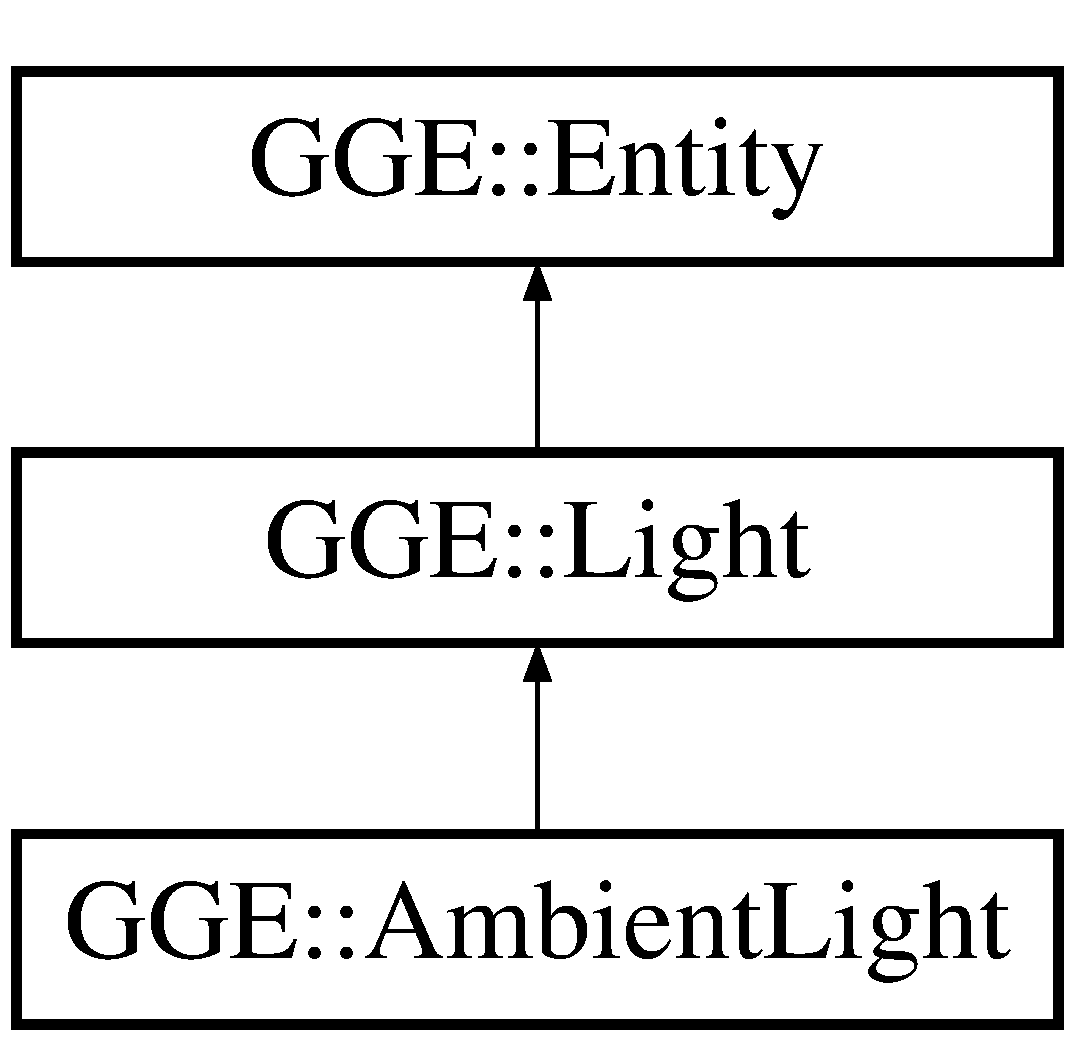
\includegraphics[height=3.000000cm]{class_g_g_e_1_1_ambient_light}
\end{center}
\end{figure}
\subsection*{Public Member Functions}
\begin{DoxyCompactItemize}
\item 
\hyperlink{class_g_g_e_1_1_ambient_light_a4cc2db326ae3316ff6a81d3b5f670b91}{Ambient\+Light} (glm\+::vec3 \hyperlink{class_g_g_e_1_1_entity_a38a9fa01bfaf37ca415181ba6a179d3f}{position}, glm\+::vec3 \hyperlink{class_g_g_e_1_1_entity_a80c69365314541244f26e4a15b4223d8}{direction}, \hyperlink{namespace_g_g_e_aff43741fd756c83cbfd5d4d5cd9fcf41}{Color4} \hyperlink{class_g_g_e_1_1_light_a4d2f4605abc44637feac0d0312ce0717}{color})
\item 
\hyperlink{class_g_g_e_1_1_ambient_light_a43219fadd4eb1069f2998ca316ef427b}{$\sim$\+Ambient\+Light} ()
\end{DoxyCompactItemize}
\subsection*{Additional Inherited Members}


\subsection{Constructor \& Destructor Documentation}
\hypertarget{class_g_g_e_1_1_ambient_light_a4cc2db326ae3316ff6a81d3b5f670b91}{\index{G\+G\+E\+::\+Ambient\+Light@{G\+G\+E\+::\+Ambient\+Light}!Ambient\+Light@{Ambient\+Light}}
\index{Ambient\+Light@{Ambient\+Light}!G\+G\+E\+::\+Ambient\+Light@{G\+G\+E\+::\+Ambient\+Light}}
\subsubsection[{Ambient\+Light}]{\setlength{\rightskip}{0pt plus 5cm}G\+G\+E\+::\+Ambient\+Light\+::\+Ambient\+Light (
\begin{DoxyParamCaption}
\item[{glm\+::vec3}]{position, }
\item[{glm\+::vec3}]{direction, }
\item[{{\bf Color4}}]{color}
\end{DoxyParamCaption}
)}}\label{class_g_g_e_1_1_ambient_light_a4cc2db326ae3316ff6a81d3b5f670b91}
\hypertarget{class_g_g_e_1_1_ambient_light_a43219fadd4eb1069f2998ca316ef427b}{\index{G\+G\+E\+::\+Ambient\+Light@{G\+G\+E\+::\+Ambient\+Light}!````~Ambient\+Light@{$\sim$\+Ambient\+Light}}
\index{````~Ambient\+Light@{$\sim$\+Ambient\+Light}!G\+G\+E\+::\+Ambient\+Light@{G\+G\+E\+::\+Ambient\+Light}}
\subsubsection[{$\sim$\+Ambient\+Light}]{\setlength{\rightskip}{0pt plus 5cm}G\+G\+E\+::\+Ambient\+Light\+::$\sim$\+Ambient\+Light (
\begin{DoxyParamCaption}
{}
\end{DoxyParamCaption}
)}}\label{class_g_g_e_1_1_ambient_light_a43219fadd4eb1069f2998ca316ef427b}


The documentation for this class was generated from the following files\+:\begin{DoxyCompactItemize}
\item 
include/\hyperlink{light_8h}{light.\+h}\item 
src/\hyperlink{light_8cpp}{light.\+cpp}\end{DoxyCompactItemize}

\hypertarget{class_g_g_e_1_1_application}{\section{G\+G\+E\+:\+:Application Class Reference}
\label{class_g_g_e_1_1_application}\index{G\+G\+E\+::\+Application@{G\+G\+E\+::\+Application}}
}


{\ttfamily \#include $<$application.\+h$>$}

\subsection*{Public Member Functions}
\begin{DoxyCompactItemize}
\item 
\hyperlink{class_g_g_e_1_1_application_ab30339d40c6eea9ddc818fb7b7f0b127}{Application} ()
\item 
\hyperlink{class_g_g_e_1_1_application_aa61a2e40680e004d1af303c9b81bd109}{$\sim$\+Application} ()
\item 
\hyperlink{class_g_g_e_1_1_window}{Window} $\ast$ \hyperlink{class_g_g_e_1_1_application_a403820d97ee74e9bab85743e651a8c8c}{add\+Window} (int height, int width, bool fullscreen, char $\ast$title, bool is\+Main)
\end{DoxyCompactItemize}
\subsection*{Static Public Member Functions}
\begin{DoxyCompactItemize}
\item 
static void \hyperlink{class_g_g_e_1_1_application_acc3c35b614352705a8e11567abba31b2}{glfw\+Error\+Callback} (int error, const char $\ast$description)
\end{DoxyCompactItemize}
\subsection*{Public Attributes}
\begin{DoxyCompactItemize}
\item 
\hyperlink{class_g_g_e_1_1_window}{Window} $\ast$ \hyperlink{class_g_g_e_1_1_application_afac18c3566e0934960cf292bef534fe6}{windows}
\end{DoxyCompactItemize}
\subsection*{Static Public Attributes}
\begin{DoxyCompactItemize}
\item 
static \hyperlink{class_g_g_e_1_1_window}{Window} $\ast$ \hyperlink{class_g_g_e_1_1_application_a9c9cce3ea5902ce5c8fac386d4592e41}{main\+Window} = N\+U\+L\+L
\item 
static bool \hyperlink{class_g_g_e_1_1_application_a3aa0cfc5ba81457e511130b8fddb0788}{glew\+Initialized} = false
\end{DoxyCompactItemize}
\subsection*{Private Types}
\begin{DoxyCompactItemize}
\item 
enum \hyperlink{class_g_g_e_1_1_application_a39cb0a658b749fd014b3355c157d267b}{Error\+Code} \{ \hyperlink{class_g_g_e_1_1_application_a39cb0a658b749fd014b3355c157d267ba0af907f479a06dc7053089d490fbf955}{G\+L\+F\+W\+\_\+\+I\+N\+I\+T\+\_\+\+F\+A\+I\+L\+U\+R\+E}, 
\hyperlink{class_g_g_e_1_1_application_a39cb0a658b749fd014b3355c157d267ba09d66e7a4f11315fe476637fb687207f}{G\+L\+E\+W\+\_\+\+I\+N\+I\+T\+\_\+\+F\+A\+I\+L\+U\+R\+E}, 
\hyperlink{class_g_g_e_1_1_application_a39cb0a658b749fd014b3355c157d267ba740a2252d9dc7e54920205d1f28eb6a9}{C\+R\+E\+A\+T\+E\+\_\+\+W\+I\+N\+D\+O\+W\+\_\+\+F\+A\+I\+L\+U\+R\+E}, 
\hyperlink{class_g_g_e_1_1_application_a39cb0a658b749fd014b3355c157d267ba4a9d849e8ef967cc1138df428af830bb}{S\+U\+C\+C\+E\+S\+S}
 \}
\end{DoxyCompactItemize}
\subsection*{Private Member Functions}
\begin{DoxyCompactItemize}
\item 
int \hyperlink{class_g_g_e_1_1_application_a79675202f34d2d8105fbecb2ecc35db0}{init} ()
\item 
void \hyperlink{class_g_g_e_1_1_application_a9aa875072c65b2b59b1cbf231a949d21}{terminate} (\hyperlink{class_g_g_e_1_1_application_a39cb0a658b749fd014b3355c157d267b}{Error\+Code} e)
\end{DoxyCompactItemize}


\subsection{Member Enumeration Documentation}
\hypertarget{class_g_g_e_1_1_application_a39cb0a658b749fd014b3355c157d267b}{\index{G\+G\+E\+::\+Application@{G\+G\+E\+::\+Application}!Error\+Code@{Error\+Code}}
\index{Error\+Code@{Error\+Code}!G\+G\+E\+::\+Application@{G\+G\+E\+::\+Application}}
\subsubsection[{Error\+Code}]{\setlength{\rightskip}{0pt plus 5cm}enum {\bf G\+G\+E\+::\+Application\+::\+Error\+Code}\hspace{0.3cm}{\ttfamily [private]}}}\label{class_g_g_e_1_1_application_a39cb0a658b749fd014b3355c157d267b}
\begin{Desc}
\item[Enumerator]\par
\begin{description}
\index{G\+L\+F\+W\+\_\+\+I\+N\+I\+T\+\_\+\+F\+A\+I\+L\+U\+R\+E@{G\+L\+F\+W\+\_\+\+I\+N\+I\+T\+\_\+\+F\+A\+I\+L\+U\+R\+E}!G\+G\+E\+::\+Application@{G\+G\+E\+::\+Application}}\index{G\+G\+E\+::\+Application@{G\+G\+E\+::\+Application}!G\+L\+F\+W\+\_\+\+I\+N\+I\+T\+\_\+\+F\+A\+I\+L\+U\+R\+E@{G\+L\+F\+W\+\_\+\+I\+N\+I\+T\+\_\+\+F\+A\+I\+L\+U\+R\+E}}\item[{\em 
\hypertarget{class_g_g_e_1_1_application_a39cb0a658b749fd014b3355c157d267ba0af907f479a06dc7053089d490fbf955}{G\+L\+F\+W\+\_\+\+I\+N\+I\+T\+\_\+\+F\+A\+I\+L\+U\+R\+E}\label{class_g_g_e_1_1_application_a39cb0a658b749fd014b3355c157d267ba0af907f479a06dc7053089d490fbf955}
}]\index{G\+L\+E\+W\+\_\+\+I\+N\+I\+T\+\_\+\+F\+A\+I\+L\+U\+R\+E@{G\+L\+E\+W\+\_\+\+I\+N\+I\+T\+\_\+\+F\+A\+I\+L\+U\+R\+E}!G\+G\+E\+::\+Application@{G\+G\+E\+::\+Application}}\index{G\+G\+E\+::\+Application@{G\+G\+E\+::\+Application}!G\+L\+E\+W\+\_\+\+I\+N\+I\+T\+\_\+\+F\+A\+I\+L\+U\+R\+E@{G\+L\+E\+W\+\_\+\+I\+N\+I\+T\+\_\+\+F\+A\+I\+L\+U\+R\+E}}\item[{\em 
\hypertarget{class_g_g_e_1_1_application_a39cb0a658b749fd014b3355c157d267ba09d66e7a4f11315fe476637fb687207f}{G\+L\+E\+W\+\_\+\+I\+N\+I\+T\+\_\+\+F\+A\+I\+L\+U\+R\+E}\label{class_g_g_e_1_1_application_a39cb0a658b749fd014b3355c157d267ba09d66e7a4f11315fe476637fb687207f}
}]\index{C\+R\+E\+A\+T\+E\+\_\+\+W\+I\+N\+D\+O\+W\+\_\+\+F\+A\+I\+L\+U\+R\+E@{C\+R\+E\+A\+T\+E\+\_\+\+W\+I\+N\+D\+O\+W\+\_\+\+F\+A\+I\+L\+U\+R\+E}!G\+G\+E\+::\+Application@{G\+G\+E\+::\+Application}}\index{G\+G\+E\+::\+Application@{G\+G\+E\+::\+Application}!C\+R\+E\+A\+T\+E\+\_\+\+W\+I\+N\+D\+O\+W\+\_\+\+F\+A\+I\+L\+U\+R\+E@{C\+R\+E\+A\+T\+E\+\_\+\+W\+I\+N\+D\+O\+W\+\_\+\+F\+A\+I\+L\+U\+R\+E}}\item[{\em 
\hypertarget{class_g_g_e_1_1_application_a39cb0a658b749fd014b3355c157d267ba740a2252d9dc7e54920205d1f28eb6a9}{C\+R\+E\+A\+T\+E\+\_\+\+W\+I\+N\+D\+O\+W\+\_\+\+F\+A\+I\+L\+U\+R\+E}\label{class_g_g_e_1_1_application_a39cb0a658b749fd014b3355c157d267ba740a2252d9dc7e54920205d1f28eb6a9}
}]\index{S\+U\+C\+C\+E\+S\+S@{S\+U\+C\+C\+E\+S\+S}!G\+G\+E\+::\+Application@{G\+G\+E\+::\+Application}}\index{G\+G\+E\+::\+Application@{G\+G\+E\+::\+Application}!S\+U\+C\+C\+E\+S\+S@{S\+U\+C\+C\+E\+S\+S}}\item[{\em 
\hypertarget{class_g_g_e_1_1_application_a39cb0a658b749fd014b3355c157d267ba4a9d849e8ef967cc1138df428af830bb}{S\+U\+C\+C\+E\+S\+S}\label{class_g_g_e_1_1_application_a39cb0a658b749fd014b3355c157d267ba4a9d849e8ef967cc1138df428af830bb}
}]\end{description}
\end{Desc}


\subsection{Constructor \& Destructor Documentation}
\hypertarget{class_g_g_e_1_1_application_ab30339d40c6eea9ddc818fb7b7f0b127}{\index{G\+G\+E\+::\+Application@{G\+G\+E\+::\+Application}!Application@{Application}}
\index{Application@{Application}!G\+G\+E\+::\+Application@{G\+G\+E\+::\+Application}}
\subsubsection[{Application}]{\setlength{\rightskip}{0pt plus 5cm}G\+G\+E\+::\+Application\+::\+Application (
\begin{DoxyParamCaption}
{}
\end{DoxyParamCaption}
)}}\label{class_g_g_e_1_1_application_ab30339d40c6eea9ddc818fb7b7f0b127}
\hypertarget{class_g_g_e_1_1_application_aa61a2e40680e004d1af303c9b81bd109}{\index{G\+G\+E\+::\+Application@{G\+G\+E\+::\+Application}!````~Application@{$\sim$\+Application}}
\index{````~Application@{$\sim$\+Application}!G\+G\+E\+::\+Application@{G\+G\+E\+::\+Application}}
\subsubsection[{$\sim$\+Application}]{\setlength{\rightskip}{0pt plus 5cm}G\+G\+E\+::\+Application\+::$\sim$\+Application (
\begin{DoxyParamCaption}
{}
\end{DoxyParamCaption}
)}}\label{class_g_g_e_1_1_application_aa61a2e40680e004d1af303c9b81bd109}


\subsection{Member Function Documentation}
\hypertarget{class_g_g_e_1_1_application_a403820d97ee74e9bab85743e651a8c8c}{\index{G\+G\+E\+::\+Application@{G\+G\+E\+::\+Application}!add\+Window@{add\+Window}}
\index{add\+Window@{add\+Window}!G\+G\+E\+::\+Application@{G\+G\+E\+::\+Application}}
\subsubsection[{add\+Window}]{\setlength{\rightskip}{0pt plus 5cm}{\bf Window} $\ast$ G\+G\+E\+::\+Application\+::add\+Window (
\begin{DoxyParamCaption}
\item[{int}]{height, }
\item[{int}]{width, }
\item[{bool}]{fullscreen, }
\item[{char $\ast$}]{title, }
\item[{bool}]{is\+Main}
\end{DoxyParamCaption}
)}}\label{class_g_g_e_1_1_application_a403820d97ee74e9bab85743e651a8c8c}
\hypertarget{class_g_g_e_1_1_application_acc3c35b614352705a8e11567abba31b2}{\index{G\+G\+E\+::\+Application@{G\+G\+E\+::\+Application}!glfw\+Error\+Callback@{glfw\+Error\+Callback}}
\index{glfw\+Error\+Callback@{glfw\+Error\+Callback}!G\+G\+E\+::\+Application@{G\+G\+E\+::\+Application}}
\subsubsection[{glfw\+Error\+Callback}]{\setlength{\rightskip}{0pt plus 5cm}void G\+G\+E\+::\+Application\+::glfw\+Error\+Callback (
\begin{DoxyParamCaption}
\item[{int}]{error, }
\item[{const char $\ast$}]{description}
\end{DoxyParamCaption}
)\hspace{0.3cm}{\ttfamily [static]}}}\label{class_g_g_e_1_1_application_acc3c35b614352705a8e11567abba31b2}
\hypertarget{class_g_g_e_1_1_application_a79675202f34d2d8105fbecb2ecc35db0}{\index{G\+G\+E\+::\+Application@{G\+G\+E\+::\+Application}!init@{init}}
\index{init@{init}!G\+G\+E\+::\+Application@{G\+G\+E\+::\+Application}}
\subsubsection[{init}]{\setlength{\rightskip}{0pt plus 5cm}int G\+G\+E\+::\+Application\+::init (
\begin{DoxyParamCaption}
{}
\end{DoxyParamCaption}
)\hspace{0.3cm}{\ttfamily [private]}}}\label{class_g_g_e_1_1_application_a79675202f34d2d8105fbecb2ecc35db0}
\hypertarget{class_g_g_e_1_1_application_a9aa875072c65b2b59b1cbf231a949d21}{\index{G\+G\+E\+::\+Application@{G\+G\+E\+::\+Application}!terminate@{terminate}}
\index{terminate@{terminate}!G\+G\+E\+::\+Application@{G\+G\+E\+::\+Application}}
\subsubsection[{terminate}]{\setlength{\rightskip}{0pt plus 5cm}void G\+G\+E\+::\+Application\+::terminate (
\begin{DoxyParamCaption}
\item[{{\bf Error\+Code}}]{e}
\end{DoxyParamCaption}
)\hspace{0.3cm}{\ttfamily [private]}}}\label{class_g_g_e_1_1_application_a9aa875072c65b2b59b1cbf231a949d21}


\subsection{Member Data Documentation}
\hypertarget{class_g_g_e_1_1_application_a3aa0cfc5ba81457e511130b8fddb0788}{\index{G\+G\+E\+::\+Application@{G\+G\+E\+::\+Application}!glew\+Initialized@{glew\+Initialized}}
\index{glew\+Initialized@{glew\+Initialized}!G\+G\+E\+::\+Application@{G\+G\+E\+::\+Application}}
\subsubsection[{glew\+Initialized}]{\setlength{\rightskip}{0pt plus 5cm}bool G\+G\+E\+::\+Application\+::glew\+Initialized = false\hspace{0.3cm}{\ttfamily [static]}}}\label{class_g_g_e_1_1_application_a3aa0cfc5ba81457e511130b8fddb0788}
\hypertarget{class_g_g_e_1_1_application_a9c9cce3ea5902ce5c8fac386d4592e41}{\index{G\+G\+E\+::\+Application@{G\+G\+E\+::\+Application}!main\+Window@{main\+Window}}
\index{main\+Window@{main\+Window}!G\+G\+E\+::\+Application@{G\+G\+E\+::\+Application}}
\subsubsection[{main\+Window}]{\setlength{\rightskip}{0pt plus 5cm}{\bf Window} $\ast$ G\+G\+E\+::\+Application\+::main\+Window = N\+U\+L\+L\hspace{0.3cm}{\ttfamily [static]}}}\label{class_g_g_e_1_1_application_a9c9cce3ea5902ce5c8fac386d4592e41}
\hypertarget{class_g_g_e_1_1_application_afac18c3566e0934960cf292bef534fe6}{\index{G\+G\+E\+::\+Application@{G\+G\+E\+::\+Application}!windows@{windows}}
\index{windows@{windows}!G\+G\+E\+::\+Application@{G\+G\+E\+::\+Application}}
\subsubsection[{windows}]{\setlength{\rightskip}{0pt plus 5cm}{\bf Window}$\ast$ G\+G\+E\+::\+Application\+::windows}}\label{class_g_g_e_1_1_application_afac18c3566e0934960cf292bef534fe6}


The documentation for this class was generated from the following files\+:\begin{DoxyCompactItemize}
\item 
include/\hyperlink{application_8h}{application.\+h}\item 
src/\hyperlink{application_8cpp}{application.\+cpp}\end{DoxyCompactItemize}

\hypertarget{class_g_g_e_1_1_camera}{\section{G\+G\+E\+:\+:Camera Class Reference}
\label{class_g_g_e_1_1_camera}\index{G\+G\+E\+::\+Camera@{G\+G\+E\+::\+Camera}}
}


{\ttfamily \#include $<$camera.\+h$>$}

Inheritance diagram for G\+G\+E\+:\+:Camera\+:\begin{figure}[H]
\begin{center}
\leavevmode
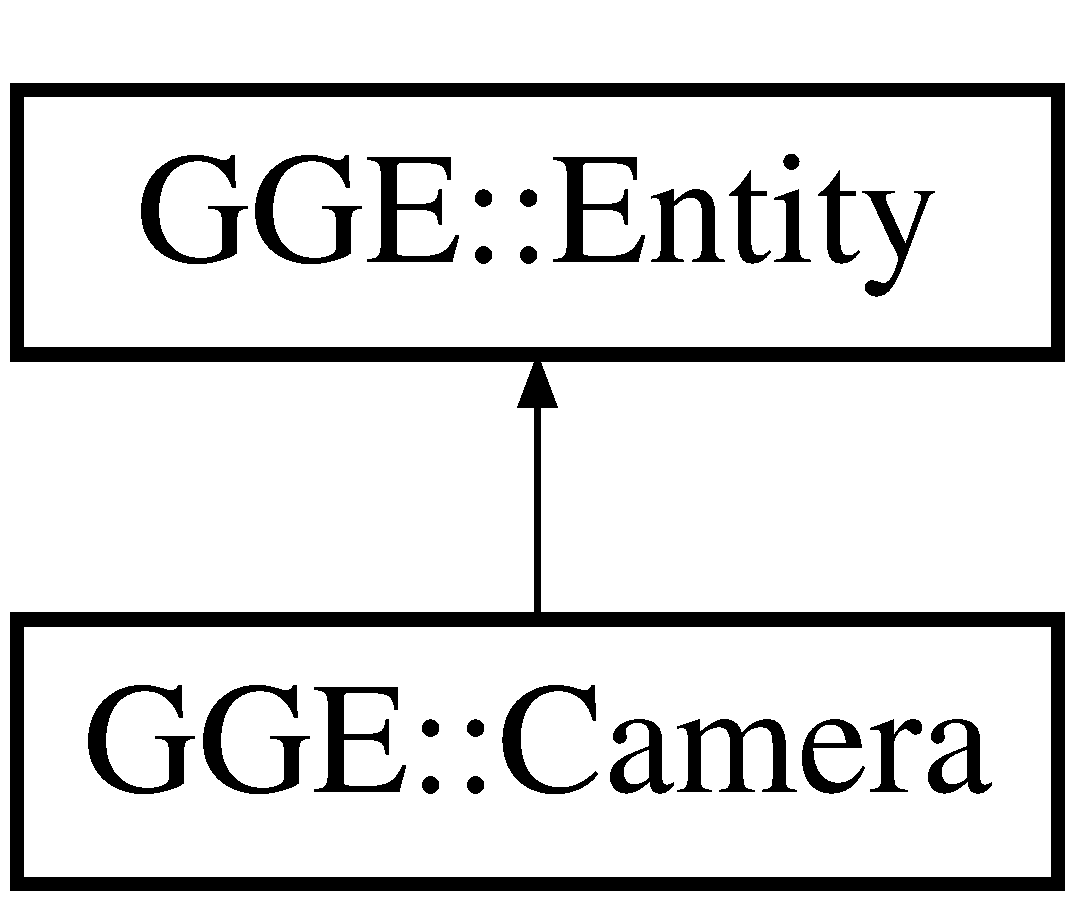
\includegraphics[height=2.000000cm]{class_g_g_e_1_1_camera}
\end{center}
\end{figure}
\subsection*{Public Member Functions}
\begin{DoxyCompactItemize}
\item 
\hyperlink{class_g_g_e_1_1_camera_a07e9334dc74b4148d1bad25585072ad4}{Camera} (glm\+::vec3 \hyperlink{class_g_g_e_1_1_entity_a38a9fa01bfaf37ca415181ba6a179d3f}{position}, glm\+::vec3 \hyperlink{class_g_g_e_1_1_entity_a80c69365314541244f26e4a15b4223d8}{direction}, glm\+::vec3 \hyperlink{class_g_g_e_1_1_camera_a48d161f43a6c2d8a39048bae3d0e1c89}{up}=\hyperlink{geometry_8h_a7d6711c6186da4b0a5340c87437ecea1}{Y\+\_\+\+U\+N\+I\+T\+\_\+\+V\+E\+C\+T\+O\+R})
\item 
\hyperlink{class_g_g_e_1_1_camera_a72d7bd6f2ed982be2d0e93f3d3ef2127}{$\sim$\+Camera} ()
\item 
\hyperlink{class_g_g_e_1_1_camera}{Camera} $\ast$ \hyperlink{class_g_g_e_1_1_camera_ac971efe3635b1496133841e5503564d3}{use} ()
\item 
glm\+::mat4 \hyperlink{class_g_g_e_1_1_camera_adcad2633fd701fffd7519c3aa2b5edc2}{get\+View\+Matrix} ()
\item 
glm\+::vec3 \hyperlink{class_g_g_e_1_1_camera_ab5a61819ea4dfa2368b099ec4cb4a9a3}{get\+Up} ()
\item 
glm\+::vec3 \hyperlink{class_g_g_e_1_1_camera_a1c3a0d332981a9ba7a07f60263bb8a3c}{get\+Right} ()
\item 
glm\+::vec3 \hyperlink{class_g_g_e_1_1_camera_aabbc2364f59c1d4a2aaf8dbde0414570}{move} (glm\+::vec3 translation)
\item 
glm\+::vec3 \hyperlink{class_g_g_e_1_1_camera_acc49c4d20d440e3602c7304518856683}{set\+Position} (glm\+::vec3 new\+Position)
\item 
glm\+::vec3 \hyperlink{class_g_g_e_1_1_camera_ab6914aa89065900c3c2509a2efa48045}{rotate} (float angle, glm\+::vec3 rotation\+Axis)
\item 
void \hyperlink{class_g_g_e_1_1_camera_abf61bb5eb074da41032e5debb30c20d9}{update\+Physics} (float delta\+Time)
\item 
glm\+::vec3 \hyperlink{class_g_g_e_1_1_camera_a09c621baf3609dadb7e83132783005da}{yaw} (float angle)
\item 
glm\+::vec3 \hyperlink{class_g_g_e_1_1_camera_a0c88a86e369cb916f91a8c0f49d6adc9}{pitch} (float angle)
\item 
glm\+::vec3 \hyperlink{class_g_g_e_1_1_camera_a1583d20af7d4388d8984ae03163cf68c}{set\+Direction} (glm\+::vec3 new\+Direction)
\end{DoxyCompactItemize}
\subsection*{Static Public Member Functions}
\begin{DoxyCompactItemize}
\item 
static \hyperlink{class_g_g_e_1_1_camera}{Camera} $\ast$ \hyperlink{class_g_g_e_1_1_camera_ae92af63f3737bc869e94e5f4703fbaa6}{get\+Current\+Camera} ()
\end{DoxyCompactItemize}
\subsection*{Private Member Functions}
\begin{DoxyCompactItemize}
\item 
void \hyperlink{class_g_g_e_1_1_camera_aba9d72d5688c3a8d7aa5eff868ef8c3b}{recalculate\+Direction} ()
\end{DoxyCompactItemize}
\subsection*{Private Attributes}
\begin{DoxyCompactItemize}
\item 
glm\+::mat4 \hyperlink{class_g_g_e_1_1_camera_a221e30f65f6ea2f56effe0f49d788a62}{view\+Matrix}
\item 
glm\+::vec3 \hyperlink{class_g_g_e_1_1_camera_a48d161f43a6c2d8a39048bae3d0e1c89}{up}
\item 
glm\+::vec3 \hyperlink{class_g_g_e_1_1_camera_af9a93409b55b7d6fcc5c6ccf20d146fe}{right}
\item 
float \hyperlink{class_g_g_e_1_1_camera_af4ce4bd9320cb90a96279e89e971f414}{horizontal\+Angle}
\item 
float \hyperlink{class_g_g_e_1_1_camera_a15ada6665d1e31494ee175f1668e7655}{vertical\+Angle}
\end{DoxyCompactItemize}
\subsection*{Static Private Attributes}
\begin{DoxyCompactItemize}
\item 
static \hyperlink{class_g_g_e_1_1_camera}{Camera} $\ast$ \hyperlink{class_g_g_e_1_1_camera_a500bf2297f52a16911d453c2d8a4dafc}{current\+Camera} = N\+U\+L\+L
\item 
static std\+::list$<$ \hyperlink{class_g_g_e_1_1_camera}{Camera} $\ast$ $>$ \hyperlink{class_g_g_e_1_1_camera_a0840a832e6d94923576520715a1e5933}{active\+Cameras}
\end{DoxyCompactItemize}
\subsection*{Additional Inherited Members}


\subsection{Constructor \& Destructor Documentation}
\hypertarget{class_g_g_e_1_1_camera_a07e9334dc74b4148d1bad25585072ad4}{\index{G\+G\+E\+::\+Camera@{G\+G\+E\+::\+Camera}!Camera@{Camera}}
\index{Camera@{Camera}!G\+G\+E\+::\+Camera@{G\+G\+E\+::\+Camera}}
\subsubsection[{Camera}]{\setlength{\rightskip}{0pt plus 5cm}G\+G\+E\+::\+Camera\+::\+Camera (
\begin{DoxyParamCaption}
\item[{glm\+::vec3}]{position, }
\item[{glm\+::vec3}]{direction, }
\item[{glm\+::vec3}]{up = {\ttfamily {\bf Y\+\_\+\+U\+N\+I\+T\+\_\+\+V\+E\+C\+T\+O\+R}}}
\end{DoxyParamCaption}
)}}\label{class_g_g_e_1_1_camera_a07e9334dc74b4148d1bad25585072ad4}
\hypertarget{class_g_g_e_1_1_camera_a72d7bd6f2ed982be2d0e93f3d3ef2127}{\index{G\+G\+E\+::\+Camera@{G\+G\+E\+::\+Camera}!````~Camera@{$\sim$\+Camera}}
\index{````~Camera@{$\sim$\+Camera}!G\+G\+E\+::\+Camera@{G\+G\+E\+::\+Camera}}
\subsubsection[{$\sim$\+Camera}]{\setlength{\rightskip}{0pt plus 5cm}G\+G\+E\+::\+Camera\+::$\sim$\+Camera (
\begin{DoxyParamCaption}
{}
\end{DoxyParamCaption}
)}}\label{class_g_g_e_1_1_camera_a72d7bd6f2ed982be2d0e93f3d3ef2127}


\subsection{Member Function Documentation}
\hypertarget{class_g_g_e_1_1_camera_ae92af63f3737bc869e94e5f4703fbaa6}{\index{G\+G\+E\+::\+Camera@{G\+G\+E\+::\+Camera}!get\+Current\+Camera@{get\+Current\+Camera}}
\index{get\+Current\+Camera@{get\+Current\+Camera}!G\+G\+E\+::\+Camera@{G\+G\+E\+::\+Camera}}
\subsubsection[{get\+Current\+Camera}]{\setlength{\rightskip}{0pt plus 5cm}{\bf Camera} $\ast$ G\+G\+E\+::\+Camera\+::get\+Current\+Camera (
\begin{DoxyParamCaption}
{}
\end{DoxyParamCaption}
)\hspace{0.3cm}{\ttfamily [static]}}}\label{class_g_g_e_1_1_camera_ae92af63f3737bc869e94e5f4703fbaa6}
\hypertarget{class_g_g_e_1_1_camera_a1c3a0d332981a9ba7a07f60263bb8a3c}{\index{G\+G\+E\+::\+Camera@{G\+G\+E\+::\+Camera}!get\+Right@{get\+Right}}
\index{get\+Right@{get\+Right}!G\+G\+E\+::\+Camera@{G\+G\+E\+::\+Camera}}
\subsubsection[{get\+Right}]{\setlength{\rightskip}{0pt plus 5cm}glm\+::vec3 G\+G\+E\+::\+Camera\+::get\+Right (
\begin{DoxyParamCaption}
{}
\end{DoxyParamCaption}
)}}\label{class_g_g_e_1_1_camera_a1c3a0d332981a9ba7a07f60263bb8a3c}
\hypertarget{class_g_g_e_1_1_camera_ab5a61819ea4dfa2368b099ec4cb4a9a3}{\index{G\+G\+E\+::\+Camera@{G\+G\+E\+::\+Camera}!get\+Up@{get\+Up}}
\index{get\+Up@{get\+Up}!G\+G\+E\+::\+Camera@{G\+G\+E\+::\+Camera}}
\subsubsection[{get\+Up}]{\setlength{\rightskip}{0pt plus 5cm}glm\+::vec3 G\+G\+E\+::\+Camera\+::get\+Up (
\begin{DoxyParamCaption}
{}
\end{DoxyParamCaption}
)}}\label{class_g_g_e_1_1_camera_ab5a61819ea4dfa2368b099ec4cb4a9a3}
\hypertarget{class_g_g_e_1_1_camera_adcad2633fd701fffd7519c3aa2b5edc2}{\index{G\+G\+E\+::\+Camera@{G\+G\+E\+::\+Camera}!get\+View\+Matrix@{get\+View\+Matrix}}
\index{get\+View\+Matrix@{get\+View\+Matrix}!G\+G\+E\+::\+Camera@{G\+G\+E\+::\+Camera}}
\subsubsection[{get\+View\+Matrix}]{\setlength{\rightskip}{0pt plus 5cm}glm\+::mat4 G\+G\+E\+::\+Camera\+::get\+View\+Matrix (
\begin{DoxyParamCaption}
{}
\end{DoxyParamCaption}
)}}\label{class_g_g_e_1_1_camera_adcad2633fd701fffd7519c3aa2b5edc2}
\hypertarget{class_g_g_e_1_1_camera_aabbc2364f59c1d4a2aaf8dbde0414570}{\index{G\+G\+E\+::\+Camera@{G\+G\+E\+::\+Camera}!move@{move}}
\index{move@{move}!G\+G\+E\+::\+Camera@{G\+G\+E\+::\+Camera}}
\subsubsection[{move}]{\setlength{\rightskip}{0pt plus 5cm}glm\+::vec3 G\+G\+E\+::\+Camera\+::move (
\begin{DoxyParamCaption}
\item[{glm\+::vec3}]{translation}
\end{DoxyParamCaption}
)\hspace{0.3cm}{\ttfamily [virtual]}}}\label{class_g_g_e_1_1_camera_aabbc2364f59c1d4a2aaf8dbde0414570}


Reimplemented from \hyperlink{class_g_g_e_1_1_entity_a7525dd307ec84c0eb4052886142a57fb}{G\+G\+E\+::\+Entity}.

\hypertarget{class_g_g_e_1_1_camera_a0c88a86e369cb916f91a8c0f49d6adc9}{\index{G\+G\+E\+::\+Camera@{G\+G\+E\+::\+Camera}!pitch@{pitch}}
\index{pitch@{pitch}!G\+G\+E\+::\+Camera@{G\+G\+E\+::\+Camera}}
\subsubsection[{pitch}]{\setlength{\rightskip}{0pt plus 5cm}glm\+::vec3 G\+G\+E\+::\+Camera\+::pitch (
\begin{DoxyParamCaption}
\item[{float}]{angle}
\end{DoxyParamCaption}
)}}\label{class_g_g_e_1_1_camera_a0c88a86e369cb916f91a8c0f49d6adc9}
\hypertarget{class_g_g_e_1_1_camera_aba9d72d5688c3a8d7aa5eff868ef8c3b}{\index{G\+G\+E\+::\+Camera@{G\+G\+E\+::\+Camera}!recalculate\+Direction@{recalculate\+Direction}}
\index{recalculate\+Direction@{recalculate\+Direction}!G\+G\+E\+::\+Camera@{G\+G\+E\+::\+Camera}}
\subsubsection[{recalculate\+Direction}]{\setlength{\rightskip}{0pt plus 5cm}void G\+G\+E\+::\+Camera\+::recalculate\+Direction (
\begin{DoxyParamCaption}
{}
\end{DoxyParamCaption}
)\hspace{0.3cm}{\ttfamily [private]}}}\label{class_g_g_e_1_1_camera_aba9d72d5688c3a8d7aa5eff868ef8c3b}
\hypertarget{class_g_g_e_1_1_camera_ab6914aa89065900c3c2509a2efa48045}{\index{G\+G\+E\+::\+Camera@{G\+G\+E\+::\+Camera}!rotate@{rotate}}
\index{rotate@{rotate}!G\+G\+E\+::\+Camera@{G\+G\+E\+::\+Camera}}
\subsubsection[{rotate}]{\setlength{\rightskip}{0pt plus 5cm}glm\+::vec3 G\+G\+E\+::\+Camera\+::rotate (
\begin{DoxyParamCaption}
\item[{float}]{angle, }
\item[{glm\+::vec3}]{rotation\+Axis}
\end{DoxyParamCaption}
)\hspace{0.3cm}{\ttfamily [virtual]}}}\label{class_g_g_e_1_1_camera_ab6914aa89065900c3c2509a2efa48045}


Reimplemented from \hyperlink{class_g_g_e_1_1_entity_a98fd8225a41364d0a2d89eb0590430de}{G\+G\+E\+::\+Entity}.

\hypertarget{class_g_g_e_1_1_camera_a1583d20af7d4388d8984ae03163cf68c}{\index{G\+G\+E\+::\+Camera@{G\+G\+E\+::\+Camera}!set\+Direction@{set\+Direction}}
\index{set\+Direction@{set\+Direction}!G\+G\+E\+::\+Camera@{G\+G\+E\+::\+Camera}}
\subsubsection[{set\+Direction}]{\setlength{\rightskip}{0pt plus 5cm}glm\+::vec3 G\+G\+E\+::\+Camera\+::set\+Direction (
\begin{DoxyParamCaption}
\item[{glm\+::vec3}]{new\+Direction}
\end{DoxyParamCaption}
)\hspace{0.3cm}{\ttfamily [virtual]}}}\label{class_g_g_e_1_1_camera_a1583d20af7d4388d8984ae03163cf68c}


Reimplemented from \hyperlink{class_g_g_e_1_1_entity_a5acb66004603256c60d89253002d001c}{G\+G\+E\+::\+Entity}.

\hypertarget{class_g_g_e_1_1_camera_acc49c4d20d440e3602c7304518856683}{\index{G\+G\+E\+::\+Camera@{G\+G\+E\+::\+Camera}!set\+Position@{set\+Position}}
\index{set\+Position@{set\+Position}!G\+G\+E\+::\+Camera@{G\+G\+E\+::\+Camera}}
\subsubsection[{set\+Position}]{\setlength{\rightskip}{0pt plus 5cm}glm\+::vec3 G\+G\+E\+::\+Camera\+::set\+Position (
\begin{DoxyParamCaption}
\item[{glm\+::vec3}]{new\+Position}
\end{DoxyParamCaption}
)\hspace{0.3cm}{\ttfamily [virtual]}}}\label{class_g_g_e_1_1_camera_acc49c4d20d440e3602c7304518856683}


Reimplemented from \hyperlink{class_g_g_e_1_1_entity_a2281d937a3430a14ec23b9a10b91efcb}{G\+G\+E\+::\+Entity}.

\hypertarget{class_g_g_e_1_1_camera_abf61bb5eb074da41032e5debb30c20d9}{\index{G\+G\+E\+::\+Camera@{G\+G\+E\+::\+Camera}!update\+Physics@{update\+Physics}}
\index{update\+Physics@{update\+Physics}!G\+G\+E\+::\+Camera@{G\+G\+E\+::\+Camera}}
\subsubsection[{update\+Physics}]{\setlength{\rightskip}{0pt plus 5cm}void G\+G\+E\+::\+Camera\+::update\+Physics (
\begin{DoxyParamCaption}
\item[{float}]{delta\+Time}
\end{DoxyParamCaption}
)\hspace{0.3cm}{\ttfamily [virtual]}}}\label{class_g_g_e_1_1_camera_abf61bb5eb074da41032e5debb30c20d9}


Reimplemented from \hyperlink{class_g_g_e_1_1_entity_a22c9a6258e81ee6bd250732121e8c26f}{G\+G\+E\+::\+Entity}.

\hypertarget{class_g_g_e_1_1_camera_ac971efe3635b1496133841e5503564d3}{\index{G\+G\+E\+::\+Camera@{G\+G\+E\+::\+Camera}!use@{use}}
\index{use@{use}!G\+G\+E\+::\+Camera@{G\+G\+E\+::\+Camera}}
\subsubsection[{use}]{\setlength{\rightskip}{0pt plus 5cm}{\bf Camera} $\ast$ G\+G\+E\+::\+Camera\+::use (
\begin{DoxyParamCaption}
{}
\end{DoxyParamCaption}
)}}\label{class_g_g_e_1_1_camera_ac971efe3635b1496133841e5503564d3}
\hypertarget{class_g_g_e_1_1_camera_a09c621baf3609dadb7e83132783005da}{\index{G\+G\+E\+::\+Camera@{G\+G\+E\+::\+Camera}!yaw@{yaw}}
\index{yaw@{yaw}!G\+G\+E\+::\+Camera@{G\+G\+E\+::\+Camera}}
\subsubsection[{yaw}]{\setlength{\rightskip}{0pt plus 5cm}glm\+::vec3 G\+G\+E\+::\+Camera\+::yaw (
\begin{DoxyParamCaption}
\item[{float}]{angle}
\end{DoxyParamCaption}
)}}\label{class_g_g_e_1_1_camera_a09c621baf3609dadb7e83132783005da}


\subsection{Member Data Documentation}
\hypertarget{class_g_g_e_1_1_camera_a0840a832e6d94923576520715a1e5933}{\index{G\+G\+E\+::\+Camera@{G\+G\+E\+::\+Camera}!active\+Cameras@{active\+Cameras}}
\index{active\+Cameras@{active\+Cameras}!G\+G\+E\+::\+Camera@{G\+G\+E\+::\+Camera}}
\subsubsection[{active\+Cameras}]{\setlength{\rightskip}{0pt plus 5cm}std\+::list$<$ {\bf Camera} $\ast$ $>$ G\+G\+E\+::\+Camera\+::active\+Cameras\hspace{0.3cm}{\ttfamily [static]}, {\ttfamily [private]}}}\label{class_g_g_e_1_1_camera_a0840a832e6d94923576520715a1e5933}
\hypertarget{class_g_g_e_1_1_camera_a500bf2297f52a16911d453c2d8a4dafc}{\index{G\+G\+E\+::\+Camera@{G\+G\+E\+::\+Camera}!current\+Camera@{current\+Camera}}
\index{current\+Camera@{current\+Camera}!G\+G\+E\+::\+Camera@{G\+G\+E\+::\+Camera}}
\subsubsection[{current\+Camera}]{\setlength{\rightskip}{0pt plus 5cm}{\bf Camera} $\ast$ G\+G\+E\+::\+Camera\+::current\+Camera = N\+U\+L\+L\hspace{0.3cm}{\ttfamily [static]}, {\ttfamily [private]}}}\label{class_g_g_e_1_1_camera_a500bf2297f52a16911d453c2d8a4dafc}
\hypertarget{class_g_g_e_1_1_camera_af4ce4bd9320cb90a96279e89e971f414}{\index{G\+G\+E\+::\+Camera@{G\+G\+E\+::\+Camera}!horizontal\+Angle@{horizontal\+Angle}}
\index{horizontal\+Angle@{horizontal\+Angle}!G\+G\+E\+::\+Camera@{G\+G\+E\+::\+Camera}}
\subsubsection[{horizontal\+Angle}]{\setlength{\rightskip}{0pt plus 5cm}float G\+G\+E\+::\+Camera\+::horizontal\+Angle\hspace{0.3cm}{\ttfamily [private]}}}\label{class_g_g_e_1_1_camera_af4ce4bd9320cb90a96279e89e971f414}
\hypertarget{class_g_g_e_1_1_camera_af9a93409b55b7d6fcc5c6ccf20d146fe}{\index{G\+G\+E\+::\+Camera@{G\+G\+E\+::\+Camera}!right@{right}}
\index{right@{right}!G\+G\+E\+::\+Camera@{G\+G\+E\+::\+Camera}}
\subsubsection[{right}]{\setlength{\rightskip}{0pt plus 5cm}glm\+::vec3 G\+G\+E\+::\+Camera\+::right\hspace{0.3cm}{\ttfamily [private]}}}\label{class_g_g_e_1_1_camera_af9a93409b55b7d6fcc5c6ccf20d146fe}
\hypertarget{class_g_g_e_1_1_camera_a48d161f43a6c2d8a39048bae3d0e1c89}{\index{G\+G\+E\+::\+Camera@{G\+G\+E\+::\+Camera}!up@{up}}
\index{up@{up}!G\+G\+E\+::\+Camera@{G\+G\+E\+::\+Camera}}
\subsubsection[{up}]{\setlength{\rightskip}{0pt plus 5cm}glm\+::vec3 G\+G\+E\+::\+Camera\+::up\hspace{0.3cm}{\ttfamily [private]}}}\label{class_g_g_e_1_1_camera_a48d161f43a6c2d8a39048bae3d0e1c89}
\hypertarget{class_g_g_e_1_1_camera_a15ada6665d1e31494ee175f1668e7655}{\index{G\+G\+E\+::\+Camera@{G\+G\+E\+::\+Camera}!vertical\+Angle@{vertical\+Angle}}
\index{vertical\+Angle@{vertical\+Angle}!G\+G\+E\+::\+Camera@{G\+G\+E\+::\+Camera}}
\subsubsection[{vertical\+Angle}]{\setlength{\rightskip}{0pt plus 5cm}float G\+G\+E\+::\+Camera\+::vertical\+Angle\hspace{0.3cm}{\ttfamily [private]}}}\label{class_g_g_e_1_1_camera_a15ada6665d1e31494ee175f1668e7655}
\hypertarget{class_g_g_e_1_1_camera_a221e30f65f6ea2f56effe0f49d788a62}{\index{G\+G\+E\+::\+Camera@{G\+G\+E\+::\+Camera}!view\+Matrix@{view\+Matrix}}
\index{view\+Matrix@{view\+Matrix}!G\+G\+E\+::\+Camera@{G\+G\+E\+::\+Camera}}
\subsubsection[{view\+Matrix}]{\setlength{\rightskip}{0pt plus 5cm}glm\+::mat4 G\+G\+E\+::\+Camera\+::view\+Matrix\hspace{0.3cm}{\ttfamily [private]}}}\label{class_g_g_e_1_1_camera_a221e30f65f6ea2f56effe0f49d788a62}


The documentation for this class was generated from the following files\+:\begin{DoxyCompactItemize}
\item 
include/\hyperlink{camera_8h}{camera.\+h}\item 
src/\hyperlink{camera_8cpp}{camera.\+cpp}\end{DoxyCompactItemize}

\hypertarget{struct_g_g_e_1_1_coordinate_set}{\section{G\+G\+E\+:\+:Coordinate\+Set Struct Reference}
\label{struct_g_g_e_1_1_coordinate_set}\index{G\+G\+E\+::\+Coordinate\+Set@{G\+G\+E\+::\+Coordinate\+Set}}
}


{\ttfamily \#include $<$shape.\+h$>$}

\subsection*{Public Member Functions}
\begin{DoxyCompactItemize}
\item 
\hyperlink{struct_g_g_e_1_1_coordinate_set_a9f2b944de9803bda6a7c8a570fc846f5}{Coordinate\+Set} ()
\end{DoxyCompactItemize}
\subsection*{Public Attributes}
\begin{DoxyCompactItemize}
\item 
std\+::vector$<$ G\+Lfloat $>$ \hyperlink{struct_g_g_e_1_1_coordinate_set_aeebb89f76ea86dc1c891eca929ca4f0e}{position\+Coordinates}
\item 
std\+::vector$<$ G\+Lfloat $>$ \hyperlink{struct_g_g_e_1_1_coordinate_set_ac58dcb73dc17eb5b2cb47c47d447ffc6}{normals}
\item 
std\+::vector$<$ G\+Lfloat $>$ \hyperlink{struct_g_g_e_1_1_coordinate_set_ad4fd6c3ab0019aaaa1b6c5dce2f8ab53}{texture\+Coordinates}
\end{DoxyCompactItemize}


\subsection{Constructor \& Destructor Documentation}
\hypertarget{struct_g_g_e_1_1_coordinate_set_a9f2b944de9803bda6a7c8a570fc846f5}{\index{G\+G\+E\+::\+Coordinate\+Set@{G\+G\+E\+::\+Coordinate\+Set}!Coordinate\+Set@{Coordinate\+Set}}
\index{Coordinate\+Set@{Coordinate\+Set}!G\+G\+E\+::\+Coordinate\+Set@{G\+G\+E\+::\+Coordinate\+Set}}
\subsubsection[{Coordinate\+Set}]{\setlength{\rightskip}{0pt plus 5cm}G\+G\+E\+::\+Coordinate\+Set\+::\+Coordinate\+Set (
\begin{DoxyParamCaption}
{}
\end{DoxyParamCaption}
)\hspace{0.3cm}{\ttfamily [inline]}}}\label{struct_g_g_e_1_1_coordinate_set_a9f2b944de9803bda6a7c8a570fc846f5}


\subsection{Member Data Documentation}
\hypertarget{struct_g_g_e_1_1_coordinate_set_ac58dcb73dc17eb5b2cb47c47d447ffc6}{\index{G\+G\+E\+::\+Coordinate\+Set@{G\+G\+E\+::\+Coordinate\+Set}!normals@{normals}}
\index{normals@{normals}!G\+G\+E\+::\+Coordinate\+Set@{G\+G\+E\+::\+Coordinate\+Set}}
\subsubsection[{normals}]{\setlength{\rightskip}{0pt plus 5cm}std\+::vector$<$G\+Lfloat$>$ G\+G\+E\+::\+Coordinate\+Set\+::normals}}\label{struct_g_g_e_1_1_coordinate_set_ac58dcb73dc17eb5b2cb47c47d447ffc6}
\hypertarget{struct_g_g_e_1_1_coordinate_set_aeebb89f76ea86dc1c891eca929ca4f0e}{\index{G\+G\+E\+::\+Coordinate\+Set@{G\+G\+E\+::\+Coordinate\+Set}!position\+Coordinates@{position\+Coordinates}}
\index{position\+Coordinates@{position\+Coordinates}!G\+G\+E\+::\+Coordinate\+Set@{G\+G\+E\+::\+Coordinate\+Set}}
\subsubsection[{position\+Coordinates}]{\setlength{\rightskip}{0pt plus 5cm}std\+::vector$<$G\+Lfloat$>$ G\+G\+E\+::\+Coordinate\+Set\+::position\+Coordinates}}\label{struct_g_g_e_1_1_coordinate_set_aeebb89f76ea86dc1c891eca929ca4f0e}
\hypertarget{struct_g_g_e_1_1_coordinate_set_ad4fd6c3ab0019aaaa1b6c5dce2f8ab53}{\index{G\+G\+E\+::\+Coordinate\+Set@{G\+G\+E\+::\+Coordinate\+Set}!texture\+Coordinates@{texture\+Coordinates}}
\index{texture\+Coordinates@{texture\+Coordinates}!G\+G\+E\+::\+Coordinate\+Set@{G\+G\+E\+::\+Coordinate\+Set}}
\subsubsection[{texture\+Coordinates}]{\setlength{\rightskip}{0pt plus 5cm}std\+::vector$<$G\+Lfloat$>$ G\+G\+E\+::\+Coordinate\+Set\+::texture\+Coordinates}}\label{struct_g_g_e_1_1_coordinate_set_ad4fd6c3ab0019aaaa1b6c5dce2f8ab53}


The documentation for this struct was generated from the following file\+:\begin{DoxyCompactItemize}
\item 
include/\hyperlink{shape_8h}{shape.\+h}\end{DoxyCompactItemize}

\hypertarget{class_g_g_e_1_1_entity}{\section{G\+G\+E\+:\+:Entity Class Reference}
\label{class_g_g_e_1_1_entity}\index{G\+G\+E\+::\+Entity@{G\+G\+E\+::\+Entity}}
}


{\ttfamily \#include $<$entity.\+h$>$}

Inheritance diagram for G\+G\+E\+:\+:Entity\+:\begin{figure}[H]
\begin{center}
\leavevmode
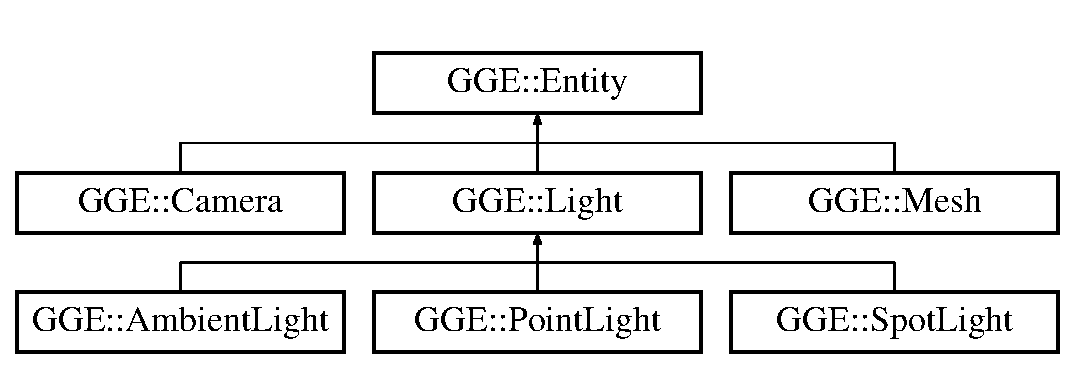
\includegraphics[height=3.000000cm]{class_g_g_e_1_1_entity}
\end{center}
\end{figure}
\subsection*{Public Member Functions}
\begin{DoxyCompactItemize}
\item 
\hyperlink{class_g_g_e_1_1_entity_ade9679d5c915b919e367d785d2a18f70}{Entity} ()
\item 
\hyperlink{class_g_g_e_1_1_entity_a18a84dee351730eac50e79d50e24f354}{Entity} (glm\+::vec3 \hyperlink{class_g_g_e_1_1_entity_a38a9fa01bfaf37ca415181ba6a179d3f}{position}, glm\+::vec3 \hyperlink{class_g_g_e_1_1_entity_a80c69365314541244f26e4a15b4223d8}{direction})
\item 
virtual \hyperlink{class_g_g_e_1_1_entity_ae9ba0e22515e35e0a6f227fb0e302304}{$\sim$\+Entity} ()
\item 
glm\+::vec3 \hyperlink{class_g_g_e_1_1_entity_a306c97f3b5a7658b3437326b4e4f1c43}{get\+Position} ()
\item 
glm\+::vec3 \hyperlink{class_g_g_e_1_1_entity_a66b3121fa59c5b3116d333f9554e5d3c}{get\+Direction} ()
\item 
glm\+::vec3 \hyperlink{class_g_g_e_1_1_entity_ad92f55ba905e45d6a5b2edea65a97174}{get\+Acceleration} ()
\item 
glm\+::vec3 \hyperlink{class_g_g_e_1_1_entity_a4efa4c353b707e71be2915199643a875}{get\+Velocity} ()
\item 
glm\+::vec3 \hyperlink{class_g_g_e_1_1_entity_aaf7d12ccb86dc8e27c0b29eb5a8b1660}{get\+Angular\+Acceleration} ()
\item 
glm\+::vec3 \hyperlink{class_g_g_e_1_1_entity_ab93e0d14ad464bf40ecbe2b0d5407547}{get\+Angular\+Velocity} ()
\item 
virtual glm\+::vec3 \hyperlink{class_g_g_e_1_1_entity_a2281d937a3430a14ec23b9a10b91efcb}{set\+Position} (glm\+::vec3 new\+Position)
\item 
virtual glm\+::vec3 \hyperlink{class_g_g_e_1_1_entity_a5acb66004603256c60d89253002d001c}{set\+Direction} (glm\+::vec3 new\+Direction)
\item 
virtual glm\+::vec3 \hyperlink{class_g_g_e_1_1_entity_a02b81e51dc7a3bc7c61da9ad67b0285a}{set\+Acceleration} (glm\+::vec3 new\+Acceleration)
\item 
virtual glm\+::vec3 \hyperlink{class_g_g_e_1_1_entity_ab787c672dea551a2033bb7c72ab28111}{set\+Velocity} (glm\+::vec3 new\+Velocity)
\item 
virtual glm\+::vec3 \hyperlink{class_g_g_e_1_1_entity_aa6a2c62a4e6ca8e32c4efdc33ce68203}{set\+Angular\+Acceleration} (glm\+::vec3 new\+Angular\+Acceleration)
\item 
virtual glm\+::vec3 \hyperlink{class_g_g_e_1_1_entity_aa92ebf0b5b04c006abfe3f36439baf75}{set\+Angular\+Velocity} (glm\+::vec3 new\+Angular\+Velocity)
\item 
virtual glm\+::vec3 \hyperlink{class_g_g_e_1_1_entity_a7525dd307ec84c0eb4052886142a57fb}{move} (glm\+::vec3 translation)
\item 
virtual glm\+::vec3 \hyperlink{class_g_g_e_1_1_entity_a98fd8225a41364d0a2d89eb0590430de}{rotate} (float angle, glm\+::vec3 rotation\+Axis)
\item 
virtual void \hyperlink{class_g_g_e_1_1_entity_a22c9a6258e81ee6bd250732121e8c26f}{update\+Physics} (float delta\+Time)
\end{DoxyCompactItemize}
\subsection*{Protected Attributes}
\begin{DoxyCompactItemize}
\item 
glm\+::vec3 \hyperlink{class_g_g_e_1_1_entity_a38a9fa01bfaf37ca415181ba6a179d3f}{position}
\item 
glm\+::vec3 \hyperlink{class_g_g_e_1_1_entity_a80c69365314541244f26e4a15b4223d8}{direction}
\item 
glm\+::vec3 \hyperlink{class_g_g_e_1_1_entity_ad27c3100a20150cc1539f1bf199f1ba3}{acceleration}
\item 
glm\+::vec3 \hyperlink{class_g_g_e_1_1_entity_a4fd6a0bab72b12da601c34e7f3fe4620}{velocity}
\item 
glm\+::vec3 \hyperlink{class_g_g_e_1_1_entity_a750368da3d794d8d1ea3a51357dcacdd}{angular\+Velocity}
\item 
glm\+::vec3 \hyperlink{class_g_g_e_1_1_entity_ae7c0ce4f2567c988b77bb3925830f946}{angular\+Acceleration}
\end{DoxyCompactItemize}


\subsection{Constructor \& Destructor Documentation}
\hypertarget{class_g_g_e_1_1_entity_ade9679d5c915b919e367d785d2a18f70}{\index{G\+G\+E\+::\+Entity@{G\+G\+E\+::\+Entity}!Entity@{Entity}}
\index{Entity@{Entity}!G\+G\+E\+::\+Entity@{G\+G\+E\+::\+Entity}}
\subsubsection[{Entity}]{\setlength{\rightskip}{0pt plus 5cm}G\+G\+E\+::\+Entity\+::\+Entity (
\begin{DoxyParamCaption}
{}
\end{DoxyParamCaption}
)}}\label{class_g_g_e_1_1_entity_ade9679d5c915b919e367d785d2a18f70}
\hypertarget{class_g_g_e_1_1_entity_a18a84dee351730eac50e79d50e24f354}{\index{G\+G\+E\+::\+Entity@{G\+G\+E\+::\+Entity}!Entity@{Entity}}
\index{Entity@{Entity}!G\+G\+E\+::\+Entity@{G\+G\+E\+::\+Entity}}
\subsubsection[{Entity}]{\setlength{\rightskip}{0pt plus 5cm}G\+G\+E\+::\+Entity\+::\+Entity (
\begin{DoxyParamCaption}
\item[{glm\+::vec3}]{position, }
\item[{glm\+::vec3}]{direction}
\end{DoxyParamCaption}
)}}\label{class_g_g_e_1_1_entity_a18a84dee351730eac50e79d50e24f354}
\hypertarget{class_g_g_e_1_1_entity_ae9ba0e22515e35e0a6f227fb0e302304}{\index{G\+G\+E\+::\+Entity@{G\+G\+E\+::\+Entity}!````~Entity@{$\sim$\+Entity}}
\index{````~Entity@{$\sim$\+Entity}!G\+G\+E\+::\+Entity@{G\+G\+E\+::\+Entity}}
\subsubsection[{$\sim$\+Entity}]{\setlength{\rightskip}{0pt plus 5cm}G\+G\+E\+::\+Entity\+::$\sim$\+Entity (
\begin{DoxyParamCaption}
{}
\end{DoxyParamCaption}
)\hspace{0.3cm}{\ttfamily [virtual]}}}\label{class_g_g_e_1_1_entity_ae9ba0e22515e35e0a6f227fb0e302304}


\subsection{Member Function Documentation}
\hypertarget{class_g_g_e_1_1_entity_ad92f55ba905e45d6a5b2edea65a97174}{\index{G\+G\+E\+::\+Entity@{G\+G\+E\+::\+Entity}!get\+Acceleration@{get\+Acceleration}}
\index{get\+Acceleration@{get\+Acceleration}!G\+G\+E\+::\+Entity@{G\+G\+E\+::\+Entity}}
\subsubsection[{get\+Acceleration}]{\setlength{\rightskip}{0pt plus 5cm}glm\+::vec3 G\+G\+E\+::\+Entity\+::get\+Acceleration (
\begin{DoxyParamCaption}
{}
\end{DoxyParamCaption}
)}}\label{class_g_g_e_1_1_entity_ad92f55ba905e45d6a5b2edea65a97174}
\hypertarget{class_g_g_e_1_1_entity_aaf7d12ccb86dc8e27c0b29eb5a8b1660}{\index{G\+G\+E\+::\+Entity@{G\+G\+E\+::\+Entity}!get\+Angular\+Acceleration@{get\+Angular\+Acceleration}}
\index{get\+Angular\+Acceleration@{get\+Angular\+Acceleration}!G\+G\+E\+::\+Entity@{G\+G\+E\+::\+Entity}}
\subsubsection[{get\+Angular\+Acceleration}]{\setlength{\rightskip}{0pt plus 5cm}glm\+::vec3 G\+G\+E\+::\+Entity\+::get\+Angular\+Acceleration (
\begin{DoxyParamCaption}
{}
\end{DoxyParamCaption}
)}}\label{class_g_g_e_1_1_entity_aaf7d12ccb86dc8e27c0b29eb5a8b1660}
\hypertarget{class_g_g_e_1_1_entity_ab93e0d14ad464bf40ecbe2b0d5407547}{\index{G\+G\+E\+::\+Entity@{G\+G\+E\+::\+Entity}!get\+Angular\+Velocity@{get\+Angular\+Velocity}}
\index{get\+Angular\+Velocity@{get\+Angular\+Velocity}!G\+G\+E\+::\+Entity@{G\+G\+E\+::\+Entity}}
\subsubsection[{get\+Angular\+Velocity}]{\setlength{\rightskip}{0pt plus 5cm}glm\+::vec3 G\+G\+E\+::\+Entity\+::get\+Angular\+Velocity (
\begin{DoxyParamCaption}
{}
\end{DoxyParamCaption}
)}}\label{class_g_g_e_1_1_entity_ab93e0d14ad464bf40ecbe2b0d5407547}
\hypertarget{class_g_g_e_1_1_entity_a66b3121fa59c5b3116d333f9554e5d3c}{\index{G\+G\+E\+::\+Entity@{G\+G\+E\+::\+Entity}!get\+Direction@{get\+Direction}}
\index{get\+Direction@{get\+Direction}!G\+G\+E\+::\+Entity@{G\+G\+E\+::\+Entity}}
\subsubsection[{get\+Direction}]{\setlength{\rightskip}{0pt plus 5cm}glm\+::vec3 G\+G\+E\+::\+Entity\+::get\+Direction (
\begin{DoxyParamCaption}
{}
\end{DoxyParamCaption}
)}}\label{class_g_g_e_1_1_entity_a66b3121fa59c5b3116d333f9554e5d3c}
\hypertarget{class_g_g_e_1_1_entity_a306c97f3b5a7658b3437326b4e4f1c43}{\index{G\+G\+E\+::\+Entity@{G\+G\+E\+::\+Entity}!get\+Position@{get\+Position}}
\index{get\+Position@{get\+Position}!G\+G\+E\+::\+Entity@{G\+G\+E\+::\+Entity}}
\subsubsection[{get\+Position}]{\setlength{\rightskip}{0pt plus 5cm}glm\+::vec3 G\+G\+E\+::\+Entity\+::get\+Position (
\begin{DoxyParamCaption}
{}
\end{DoxyParamCaption}
)}}\label{class_g_g_e_1_1_entity_a306c97f3b5a7658b3437326b4e4f1c43}
\hypertarget{class_g_g_e_1_1_entity_a4efa4c353b707e71be2915199643a875}{\index{G\+G\+E\+::\+Entity@{G\+G\+E\+::\+Entity}!get\+Velocity@{get\+Velocity}}
\index{get\+Velocity@{get\+Velocity}!G\+G\+E\+::\+Entity@{G\+G\+E\+::\+Entity}}
\subsubsection[{get\+Velocity}]{\setlength{\rightskip}{0pt plus 5cm}glm\+::vec3 G\+G\+E\+::\+Entity\+::get\+Velocity (
\begin{DoxyParamCaption}
{}
\end{DoxyParamCaption}
)}}\label{class_g_g_e_1_1_entity_a4efa4c353b707e71be2915199643a875}
\hypertarget{class_g_g_e_1_1_entity_a7525dd307ec84c0eb4052886142a57fb}{\index{G\+G\+E\+::\+Entity@{G\+G\+E\+::\+Entity}!move@{move}}
\index{move@{move}!G\+G\+E\+::\+Entity@{G\+G\+E\+::\+Entity}}
\subsubsection[{move}]{\setlength{\rightskip}{0pt plus 5cm}glm\+::vec3 G\+G\+E\+::\+Entity\+::move (
\begin{DoxyParamCaption}
\item[{glm\+::vec3}]{translation}
\end{DoxyParamCaption}
)\hspace{0.3cm}{\ttfamily [virtual]}}}\label{class_g_g_e_1_1_entity_a7525dd307ec84c0eb4052886142a57fb}


Reimplemented in \hyperlink{class_g_g_e_1_1_mesh_a40161efa046c5513710bae8db2848d20}{G\+G\+E\+::\+Mesh}, and \hyperlink{class_g_g_e_1_1_camera_aabbc2364f59c1d4a2aaf8dbde0414570}{G\+G\+E\+::\+Camera}.

\hypertarget{class_g_g_e_1_1_entity_a98fd8225a41364d0a2d89eb0590430de}{\index{G\+G\+E\+::\+Entity@{G\+G\+E\+::\+Entity}!rotate@{rotate}}
\index{rotate@{rotate}!G\+G\+E\+::\+Entity@{G\+G\+E\+::\+Entity}}
\subsubsection[{rotate}]{\setlength{\rightskip}{0pt plus 5cm}glm\+::vec3 G\+G\+E\+::\+Entity\+::rotate (
\begin{DoxyParamCaption}
\item[{float}]{angle, }
\item[{glm\+::vec3}]{rotation\+Axis}
\end{DoxyParamCaption}
)\hspace{0.3cm}{\ttfamily [virtual]}}}\label{class_g_g_e_1_1_entity_a98fd8225a41364d0a2d89eb0590430de}


Reimplemented in \hyperlink{class_g_g_e_1_1_camera_ab6914aa89065900c3c2509a2efa48045}{G\+G\+E\+::\+Camera}.

\hypertarget{class_g_g_e_1_1_entity_a02b81e51dc7a3bc7c61da9ad67b0285a}{\index{G\+G\+E\+::\+Entity@{G\+G\+E\+::\+Entity}!set\+Acceleration@{set\+Acceleration}}
\index{set\+Acceleration@{set\+Acceleration}!G\+G\+E\+::\+Entity@{G\+G\+E\+::\+Entity}}
\subsubsection[{set\+Acceleration}]{\setlength{\rightskip}{0pt plus 5cm}glm\+::vec3 G\+G\+E\+::\+Entity\+::set\+Acceleration (
\begin{DoxyParamCaption}
\item[{glm\+::vec3}]{new\+Acceleration}
\end{DoxyParamCaption}
)\hspace{0.3cm}{\ttfamily [virtual]}}}\label{class_g_g_e_1_1_entity_a02b81e51dc7a3bc7c61da9ad67b0285a}
\hypertarget{class_g_g_e_1_1_entity_aa6a2c62a4e6ca8e32c4efdc33ce68203}{\index{G\+G\+E\+::\+Entity@{G\+G\+E\+::\+Entity}!set\+Angular\+Acceleration@{set\+Angular\+Acceleration}}
\index{set\+Angular\+Acceleration@{set\+Angular\+Acceleration}!G\+G\+E\+::\+Entity@{G\+G\+E\+::\+Entity}}
\subsubsection[{set\+Angular\+Acceleration}]{\setlength{\rightskip}{0pt plus 5cm}glm\+::vec3 G\+G\+E\+::\+Entity\+::set\+Angular\+Acceleration (
\begin{DoxyParamCaption}
\item[{glm\+::vec3}]{new\+Angular\+Acceleration}
\end{DoxyParamCaption}
)\hspace{0.3cm}{\ttfamily [virtual]}}}\label{class_g_g_e_1_1_entity_aa6a2c62a4e6ca8e32c4efdc33ce68203}
\hypertarget{class_g_g_e_1_1_entity_aa92ebf0b5b04c006abfe3f36439baf75}{\index{G\+G\+E\+::\+Entity@{G\+G\+E\+::\+Entity}!set\+Angular\+Velocity@{set\+Angular\+Velocity}}
\index{set\+Angular\+Velocity@{set\+Angular\+Velocity}!G\+G\+E\+::\+Entity@{G\+G\+E\+::\+Entity}}
\subsubsection[{set\+Angular\+Velocity}]{\setlength{\rightskip}{0pt plus 5cm}glm\+::vec3 G\+G\+E\+::\+Entity\+::set\+Angular\+Velocity (
\begin{DoxyParamCaption}
\item[{glm\+::vec3}]{new\+Angular\+Velocity}
\end{DoxyParamCaption}
)\hspace{0.3cm}{\ttfamily [virtual]}}}\label{class_g_g_e_1_1_entity_aa92ebf0b5b04c006abfe3f36439baf75}
\hypertarget{class_g_g_e_1_1_entity_a5acb66004603256c60d89253002d001c}{\index{G\+G\+E\+::\+Entity@{G\+G\+E\+::\+Entity}!set\+Direction@{set\+Direction}}
\index{set\+Direction@{set\+Direction}!G\+G\+E\+::\+Entity@{G\+G\+E\+::\+Entity}}
\subsubsection[{set\+Direction}]{\setlength{\rightskip}{0pt plus 5cm}glm\+::vec3 G\+G\+E\+::\+Entity\+::set\+Direction (
\begin{DoxyParamCaption}
\item[{glm\+::vec3}]{new\+Direction}
\end{DoxyParamCaption}
)\hspace{0.3cm}{\ttfamily [virtual]}}}\label{class_g_g_e_1_1_entity_a5acb66004603256c60d89253002d001c}


Reimplemented in \hyperlink{class_g_g_e_1_1_camera_a1583d20af7d4388d8984ae03163cf68c}{G\+G\+E\+::\+Camera}.

\hypertarget{class_g_g_e_1_1_entity_a2281d937a3430a14ec23b9a10b91efcb}{\index{G\+G\+E\+::\+Entity@{G\+G\+E\+::\+Entity}!set\+Position@{set\+Position}}
\index{set\+Position@{set\+Position}!G\+G\+E\+::\+Entity@{G\+G\+E\+::\+Entity}}
\subsubsection[{set\+Position}]{\setlength{\rightskip}{0pt plus 5cm}glm\+::vec3 G\+G\+E\+::\+Entity\+::set\+Position (
\begin{DoxyParamCaption}
\item[{glm\+::vec3}]{new\+Position}
\end{DoxyParamCaption}
)\hspace{0.3cm}{\ttfamily [virtual]}}}\label{class_g_g_e_1_1_entity_a2281d937a3430a14ec23b9a10b91efcb}


Reimplemented in \hyperlink{class_g_g_e_1_1_mesh_a96e3bdea0c48b75b858261e0a6ac1eb6}{G\+G\+E\+::\+Mesh}, and \hyperlink{class_g_g_e_1_1_camera_acc49c4d20d440e3602c7304518856683}{G\+G\+E\+::\+Camera}.

\hypertarget{class_g_g_e_1_1_entity_ab787c672dea551a2033bb7c72ab28111}{\index{G\+G\+E\+::\+Entity@{G\+G\+E\+::\+Entity}!set\+Velocity@{set\+Velocity}}
\index{set\+Velocity@{set\+Velocity}!G\+G\+E\+::\+Entity@{G\+G\+E\+::\+Entity}}
\subsubsection[{set\+Velocity}]{\setlength{\rightskip}{0pt plus 5cm}glm\+::vec3 G\+G\+E\+::\+Entity\+::set\+Velocity (
\begin{DoxyParamCaption}
\item[{glm\+::vec3}]{new\+Velocity}
\end{DoxyParamCaption}
)\hspace{0.3cm}{\ttfamily [virtual]}}}\label{class_g_g_e_1_1_entity_ab787c672dea551a2033bb7c72ab28111}
\hypertarget{class_g_g_e_1_1_entity_a22c9a6258e81ee6bd250732121e8c26f}{\index{G\+G\+E\+::\+Entity@{G\+G\+E\+::\+Entity}!update\+Physics@{update\+Physics}}
\index{update\+Physics@{update\+Physics}!G\+G\+E\+::\+Entity@{G\+G\+E\+::\+Entity}}
\subsubsection[{update\+Physics}]{\setlength{\rightskip}{0pt plus 5cm}void G\+G\+E\+::\+Entity\+::update\+Physics (
\begin{DoxyParamCaption}
\item[{float}]{delta\+Time}
\end{DoxyParamCaption}
)\hspace{0.3cm}{\ttfamily [virtual]}}}\label{class_g_g_e_1_1_entity_a22c9a6258e81ee6bd250732121e8c26f}


Reimplemented in \hyperlink{class_g_g_e_1_1_camera_abf61bb5eb074da41032e5debb30c20d9}{G\+G\+E\+::\+Camera}.



\subsection{Member Data Documentation}
\hypertarget{class_g_g_e_1_1_entity_ad27c3100a20150cc1539f1bf199f1ba3}{\index{G\+G\+E\+::\+Entity@{G\+G\+E\+::\+Entity}!acceleration@{acceleration}}
\index{acceleration@{acceleration}!G\+G\+E\+::\+Entity@{G\+G\+E\+::\+Entity}}
\subsubsection[{acceleration}]{\setlength{\rightskip}{0pt plus 5cm}glm\+::vec3 G\+G\+E\+::\+Entity\+::acceleration\hspace{0.3cm}{\ttfamily [protected]}}}\label{class_g_g_e_1_1_entity_ad27c3100a20150cc1539f1bf199f1ba3}
\hypertarget{class_g_g_e_1_1_entity_ae7c0ce4f2567c988b77bb3925830f946}{\index{G\+G\+E\+::\+Entity@{G\+G\+E\+::\+Entity}!angular\+Acceleration@{angular\+Acceleration}}
\index{angular\+Acceleration@{angular\+Acceleration}!G\+G\+E\+::\+Entity@{G\+G\+E\+::\+Entity}}
\subsubsection[{angular\+Acceleration}]{\setlength{\rightskip}{0pt plus 5cm}glm\+::vec3 G\+G\+E\+::\+Entity\+::angular\+Acceleration\hspace{0.3cm}{\ttfamily [protected]}}}\label{class_g_g_e_1_1_entity_ae7c0ce4f2567c988b77bb3925830f946}
\hypertarget{class_g_g_e_1_1_entity_a750368da3d794d8d1ea3a51357dcacdd}{\index{G\+G\+E\+::\+Entity@{G\+G\+E\+::\+Entity}!angular\+Velocity@{angular\+Velocity}}
\index{angular\+Velocity@{angular\+Velocity}!G\+G\+E\+::\+Entity@{G\+G\+E\+::\+Entity}}
\subsubsection[{angular\+Velocity}]{\setlength{\rightskip}{0pt plus 5cm}glm\+::vec3 G\+G\+E\+::\+Entity\+::angular\+Velocity\hspace{0.3cm}{\ttfamily [protected]}}}\label{class_g_g_e_1_1_entity_a750368da3d794d8d1ea3a51357dcacdd}
\hypertarget{class_g_g_e_1_1_entity_a80c69365314541244f26e4a15b4223d8}{\index{G\+G\+E\+::\+Entity@{G\+G\+E\+::\+Entity}!direction@{direction}}
\index{direction@{direction}!G\+G\+E\+::\+Entity@{G\+G\+E\+::\+Entity}}
\subsubsection[{direction}]{\setlength{\rightskip}{0pt plus 5cm}glm\+::vec3 G\+G\+E\+::\+Entity\+::direction\hspace{0.3cm}{\ttfamily [protected]}}}\label{class_g_g_e_1_1_entity_a80c69365314541244f26e4a15b4223d8}
\hypertarget{class_g_g_e_1_1_entity_a38a9fa01bfaf37ca415181ba6a179d3f}{\index{G\+G\+E\+::\+Entity@{G\+G\+E\+::\+Entity}!position@{position}}
\index{position@{position}!G\+G\+E\+::\+Entity@{G\+G\+E\+::\+Entity}}
\subsubsection[{position}]{\setlength{\rightskip}{0pt plus 5cm}glm\+::vec3 G\+G\+E\+::\+Entity\+::position\hspace{0.3cm}{\ttfamily [protected]}}}\label{class_g_g_e_1_1_entity_a38a9fa01bfaf37ca415181ba6a179d3f}
\hypertarget{class_g_g_e_1_1_entity_a4fd6a0bab72b12da601c34e7f3fe4620}{\index{G\+G\+E\+::\+Entity@{G\+G\+E\+::\+Entity}!velocity@{velocity}}
\index{velocity@{velocity}!G\+G\+E\+::\+Entity@{G\+G\+E\+::\+Entity}}
\subsubsection[{velocity}]{\setlength{\rightskip}{0pt plus 5cm}glm\+::vec3 G\+G\+E\+::\+Entity\+::velocity\hspace{0.3cm}{\ttfamily [protected]}}}\label{class_g_g_e_1_1_entity_a4fd6a0bab72b12da601c34e7f3fe4620}


The documentation for this class was generated from the following files\+:\begin{DoxyCompactItemize}
\item 
include/\hyperlink{entity_8h}{entity.\+h}\item 
src/\hyperlink{entity_8cpp}{entity.\+cpp}\end{DoxyCompactItemize}

\hypertarget{class_g_g_e_1_1_light}{\section{G\+G\+E\+:\+:Light Class Reference}
\label{class_g_g_e_1_1_light}\index{G\+G\+E\+::\+Light@{G\+G\+E\+::\+Light}}
}


{\ttfamily \#include $<$light.\+h$>$}

Inheritance diagram for G\+G\+E\+:\+:Light\+:\begin{figure}[H]
\begin{center}
\leavevmode
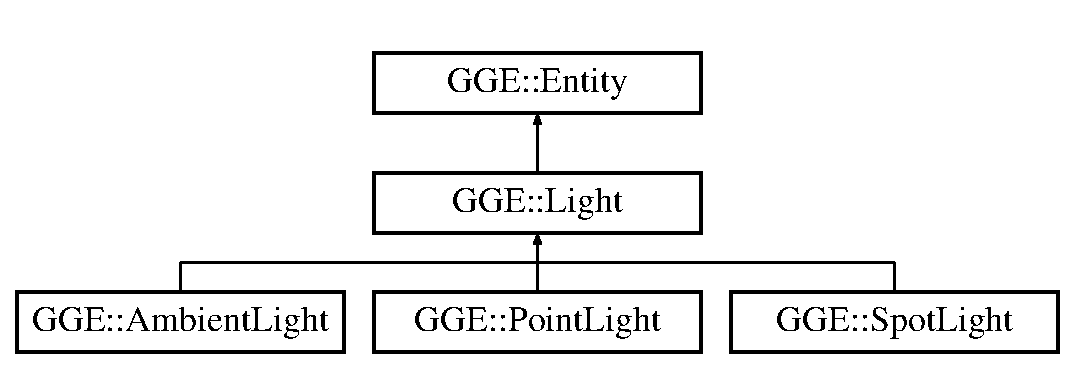
\includegraphics[height=3.000000cm]{class_g_g_e_1_1_light}
\end{center}
\end{figure}
\subsection*{Public Member Functions}
\begin{DoxyCompactItemize}
\item 
\hyperlink{class_g_g_e_1_1_light_ac10d3c4648c68b6f9ecc08b6aaa54736}{Light} ()
\item 
\hyperlink{class_g_g_e_1_1_light_ad1b55887fedae158ebf806f3858e9a10}{Light} (glm\+::vec3 \hyperlink{class_g_g_e_1_1_entity_a38a9fa01bfaf37ca415181ba6a179d3f}{position}, glm\+::vec3 \hyperlink{class_g_g_e_1_1_entity_a80c69365314541244f26e4a15b4223d8}{direction}, \hyperlink{namespace_g_g_e_abf6b28d5fd20f356a5ad88fec0789eff}{Light\+Type} \hyperlink{class_g_g_e_1_1_light_ae4d6aecd16e4e8ec0d1601acaa71400d}{type}, \hyperlink{namespace_g_g_e_aff43741fd756c83cbfd5d4d5cd9fcf41}{Color4} \hyperlink{class_g_g_e_1_1_light_a4d2f4605abc44637feac0d0312ce0717}{color})
\item 
virtual \hyperlink{class_g_g_e_1_1_light_a0bafb0a9f8f149d31ab109eb208dbef2}{$\sim$\+Light} ()
\item 
\hyperlink{namespace_g_g_e_aff43741fd756c83cbfd5d4d5cd9fcf41}{Color4} \hyperlink{class_g_g_e_1_1_light_aaedc1c8a70cd6c65651b64d648590d61}{get\+Color} ()
\item 
\hyperlink{namespace_g_g_e_abf6b28d5fd20f356a5ad88fec0789eff}{Light\+Type} \hyperlink{class_g_g_e_1_1_light_a6aa80e3d94ede0f9d6f821580ad4f015}{get\+Light\+Type} ()
\end{DoxyCompactItemize}
\subsection*{Protected Attributes}
\begin{DoxyCompactItemize}
\item 
\hyperlink{namespace_g_g_e_aff43741fd756c83cbfd5d4d5cd9fcf41}{Color4} \hyperlink{class_g_g_e_1_1_light_a4d2f4605abc44637feac0d0312ce0717}{color}
\item 
\hyperlink{namespace_g_g_e_abf6b28d5fd20f356a5ad88fec0789eff}{Light\+Type} \hyperlink{class_g_g_e_1_1_light_ae4d6aecd16e4e8ec0d1601acaa71400d}{type}
\end{DoxyCompactItemize}


\subsection{Constructor \& Destructor Documentation}
\hypertarget{class_g_g_e_1_1_light_ac10d3c4648c68b6f9ecc08b6aaa54736}{\index{G\+G\+E\+::\+Light@{G\+G\+E\+::\+Light}!Light@{Light}}
\index{Light@{Light}!G\+G\+E\+::\+Light@{G\+G\+E\+::\+Light}}
\subsubsection[{Light}]{\setlength{\rightskip}{0pt plus 5cm}G\+G\+E\+::\+Light\+::\+Light (
\begin{DoxyParamCaption}
{}
\end{DoxyParamCaption}
)}}\label{class_g_g_e_1_1_light_ac10d3c4648c68b6f9ecc08b6aaa54736}
\hypertarget{class_g_g_e_1_1_light_ad1b55887fedae158ebf806f3858e9a10}{\index{G\+G\+E\+::\+Light@{G\+G\+E\+::\+Light}!Light@{Light}}
\index{Light@{Light}!G\+G\+E\+::\+Light@{G\+G\+E\+::\+Light}}
\subsubsection[{Light}]{\setlength{\rightskip}{0pt plus 5cm}G\+G\+E\+::\+Light\+::\+Light (
\begin{DoxyParamCaption}
\item[{glm\+::vec3}]{position, }
\item[{glm\+::vec3}]{direction, }
\item[{{\bf Light\+Type}}]{type, }
\item[{{\bf Color4}}]{color}
\end{DoxyParamCaption}
)}}\label{class_g_g_e_1_1_light_ad1b55887fedae158ebf806f3858e9a10}
\hypertarget{class_g_g_e_1_1_light_a0bafb0a9f8f149d31ab109eb208dbef2}{\index{G\+G\+E\+::\+Light@{G\+G\+E\+::\+Light}!````~Light@{$\sim$\+Light}}
\index{````~Light@{$\sim$\+Light}!G\+G\+E\+::\+Light@{G\+G\+E\+::\+Light}}
\subsubsection[{$\sim$\+Light}]{\setlength{\rightskip}{0pt plus 5cm}G\+G\+E\+::\+Light\+::$\sim$\+Light (
\begin{DoxyParamCaption}
{}
\end{DoxyParamCaption}
)\hspace{0.3cm}{\ttfamily [virtual]}}}\label{class_g_g_e_1_1_light_a0bafb0a9f8f149d31ab109eb208dbef2}


\subsection{Member Function Documentation}
\hypertarget{class_g_g_e_1_1_light_aaedc1c8a70cd6c65651b64d648590d61}{\index{G\+G\+E\+::\+Light@{G\+G\+E\+::\+Light}!get\+Color@{get\+Color}}
\index{get\+Color@{get\+Color}!G\+G\+E\+::\+Light@{G\+G\+E\+::\+Light}}
\subsubsection[{get\+Color}]{\setlength{\rightskip}{0pt plus 5cm}{\bf Color4} G\+G\+E\+::\+Light\+::get\+Color (
\begin{DoxyParamCaption}
{}
\end{DoxyParamCaption}
)}}\label{class_g_g_e_1_1_light_aaedc1c8a70cd6c65651b64d648590d61}
\hypertarget{class_g_g_e_1_1_light_a6aa80e3d94ede0f9d6f821580ad4f015}{\index{G\+G\+E\+::\+Light@{G\+G\+E\+::\+Light}!get\+Light\+Type@{get\+Light\+Type}}
\index{get\+Light\+Type@{get\+Light\+Type}!G\+G\+E\+::\+Light@{G\+G\+E\+::\+Light}}
\subsubsection[{get\+Light\+Type}]{\setlength{\rightskip}{0pt plus 5cm}{\bf Light\+Type} G\+G\+E\+::\+Light\+::get\+Light\+Type (
\begin{DoxyParamCaption}
{}
\end{DoxyParamCaption}
)}}\label{class_g_g_e_1_1_light_a6aa80e3d94ede0f9d6f821580ad4f015}


\subsection{Member Data Documentation}
\hypertarget{class_g_g_e_1_1_light_a4d2f4605abc44637feac0d0312ce0717}{\index{G\+G\+E\+::\+Light@{G\+G\+E\+::\+Light}!color@{color}}
\index{color@{color}!G\+G\+E\+::\+Light@{G\+G\+E\+::\+Light}}
\subsubsection[{color}]{\setlength{\rightskip}{0pt plus 5cm}{\bf Color4} G\+G\+E\+::\+Light\+::color\hspace{0.3cm}{\ttfamily [protected]}}}\label{class_g_g_e_1_1_light_a4d2f4605abc44637feac0d0312ce0717}
\hypertarget{class_g_g_e_1_1_light_ae4d6aecd16e4e8ec0d1601acaa71400d}{\index{G\+G\+E\+::\+Light@{G\+G\+E\+::\+Light}!type@{type}}
\index{type@{type}!G\+G\+E\+::\+Light@{G\+G\+E\+::\+Light}}
\subsubsection[{type}]{\setlength{\rightskip}{0pt plus 5cm}{\bf Light\+Type} G\+G\+E\+::\+Light\+::type\hspace{0.3cm}{\ttfamily [protected]}}}\label{class_g_g_e_1_1_light_ae4d6aecd16e4e8ec0d1601acaa71400d}


The documentation for this class was generated from the following files\+:\begin{DoxyCompactItemize}
\item 
include/\hyperlink{light_8h}{light.\+h}\item 
src/\hyperlink{light_8cpp}{light.\+cpp}\end{DoxyCompactItemize}

\hypertarget{struct_g_g_e_1_1_lighting_properties}{\section{G\+G\+E\+:\+:Lighting\+Properties Struct Reference}
\label{struct_g_g_e_1_1_lighting_properties}\index{G\+G\+E\+::\+Lighting\+Properties@{G\+G\+E\+::\+Lighting\+Properties}}
}


{\ttfamily \#include $<$material.\+h$>$}

\subsection*{Public Member Functions}
\begin{DoxyCompactItemize}
\item 
\hyperlink{struct_g_g_e_1_1_lighting_properties_ad42277828655d1158b45a3ed6e032860}{Lighting\+Properties} ()
\end{DoxyCompactItemize}
\subsection*{Public Attributes}
\begin{DoxyCompactItemize}
\item 
\hyperlink{namespace_g_g_e_ae2829723f010eeffbb96282f99792546}{Color3} \hyperlink{struct_g_g_e_1_1_lighting_properties_abc31745b5f2c2a56751c0787cc8d7748}{ambient\+Color}
\item 
\hyperlink{namespace_g_g_e_ae2829723f010eeffbb96282f99792546}{Color3} \hyperlink{struct_g_g_e_1_1_lighting_properties_a74a1886610cbeafdf5749abffac3f7fe}{diffuse\+Color}
\item 
\hyperlink{namespace_g_g_e_ae2829723f010eeffbb96282f99792546}{Color3} \hyperlink{struct_g_g_e_1_1_lighting_properties_a84af66209276135e13bc63f2b407e476}{specular\+Color}
\item 
\hyperlink{namespace_g_g_e_ae2829723f010eeffbb96282f99792546}{Color3} \hyperlink{struct_g_g_e_1_1_lighting_properties_ab454f09312d4c7e3a094ba7c1aa0bfe2}{transmission\+Color}
\item 
\hyperlink{namespace_g_g_e_ae2829723f010eeffbb96282f99792546}{Color3} \hyperlink{struct_g_g_e_1_1_lighting_properties_ad5af1aadda202f0defa618fd95d47af1}{emission\+Color}
\item 
float \hyperlink{struct_g_g_e_1_1_lighting_properties_ad8ec641aa98b22f469c31724caadb5be}{shininess}
\item 
float \hyperlink{struct_g_g_e_1_1_lighting_properties_a0cd99cfbc8d9cdc491e1d6dd6c062730}{index\+Of\+Refraction}
\item 
float \hyperlink{struct_g_g_e_1_1_lighting_properties_af6a342f051cdb44d1a43534c7709f700}{dissolve}
\item 
int \hyperlink{struct_g_g_e_1_1_lighting_properties_a9ba99a712da14ece6ce4f3139e29a145}{illumination\+Model}
\end{DoxyCompactItemize}


\subsection{Constructor \& Destructor Documentation}
\hypertarget{struct_g_g_e_1_1_lighting_properties_ad42277828655d1158b45a3ed6e032860}{\index{G\+G\+E\+::\+Lighting\+Properties@{G\+G\+E\+::\+Lighting\+Properties}!Lighting\+Properties@{Lighting\+Properties}}
\index{Lighting\+Properties@{Lighting\+Properties}!G\+G\+E\+::\+Lighting\+Properties@{G\+G\+E\+::\+Lighting\+Properties}}
\subsubsection[{Lighting\+Properties}]{\setlength{\rightskip}{0pt plus 5cm}G\+G\+E\+::\+Lighting\+Properties\+::\+Lighting\+Properties (
\begin{DoxyParamCaption}
{}
\end{DoxyParamCaption}
)\hspace{0.3cm}{\ttfamily [inline]}}}\label{struct_g_g_e_1_1_lighting_properties_ad42277828655d1158b45a3ed6e032860}


\subsection{Member Data Documentation}
\hypertarget{struct_g_g_e_1_1_lighting_properties_abc31745b5f2c2a56751c0787cc8d7748}{\index{G\+G\+E\+::\+Lighting\+Properties@{G\+G\+E\+::\+Lighting\+Properties}!ambient\+Color@{ambient\+Color}}
\index{ambient\+Color@{ambient\+Color}!G\+G\+E\+::\+Lighting\+Properties@{G\+G\+E\+::\+Lighting\+Properties}}
\subsubsection[{ambient\+Color}]{\setlength{\rightskip}{0pt plus 5cm}{\bf Color3} G\+G\+E\+::\+Lighting\+Properties\+::ambient\+Color}}\label{struct_g_g_e_1_1_lighting_properties_abc31745b5f2c2a56751c0787cc8d7748}
\hypertarget{struct_g_g_e_1_1_lighting_properties_a74a1886610cbeafdf5749abffac3f7fe}{\index{G\+G\+E\+::\+Lighting\+Properties@{G\+G\+E\+::\+Lighting\+Properties}!diffuse\+Color@{diffuse\+Color}}
\index{diffuse\+Color@{diffuse\+Color}!G\+G\+E\+::\+Lighting\+Properties@{G\+G\+E\+::\+Lighting\+Properties}}
\subsubsection[{diffuse\+Color}]{\setlength{\rightskip}{0pt plus 5cm}{\bf Color3} G\+G\+E\+::\+Lighting\+Properties\+::diffuse\+Color}}\label{struct_g_g_e_1_1_lighting_properties_a74a1886610cbeafdf5749abffac3f7fe}
\hypertarget{struct_g_g_e_1_1_lighting_properties_af6a342f051cdb44d1a43534c7709f700}{\index{G\+G\+E\+::\+Lighting\+Properties@{G\+G\+E\+::\+Lighting\+Properties}!dissolve@{dissolve}}
\index{dissolve@{dissolve}!G\+G\+E\+::\+Lighting\+Properties@{G\+G\+E\+::\+Lighting\+Properties}}
\subsubsection[{dissolve}]{\setlength{\rightskip}{0pt plus 5cm}float G\+G\+E\+::\+Lighting\+Properties\+::dissolve}}\label{struct_g_g_e_1_1_lighting_properties_af6a342f051cdb44d1a43534c7709f700}
\hypertarget{struct_g_g_e_1_1_lighting_properties_ad5af1aadda202f0defa618fd95d47af1}{\index{G\+G\+E\+::\+Lighting\+Properties@{G\+G\+E\+::\+Lighting\+Properties}!emission\+Color@{emission\+Color}}
\index{emission\+Color@{emission\+Color}!G\+G\+E\+::\+Lighting\+Properties@{G\+G\+E\+::\+Lighting\+Properties}}
\subsubsection[{emission\+Color}]{\setlength{\rightskip}{0pt plus 5cm}{\bf Color3} G\+G\+E\+::\+Lighting\+Properties\+::emission\+Color}}\label{struct_g_g_e_1_1_lighting_properties_ad5af1aadda202f0defa618fd95d47af1}
\hypertarget{struct_g_g_e_1_1_lighting_properties_a9ba99a712da14ece6ce4f3139e29a145}{\index{G\+G\+E\+::\+Lighting\+Properties@{G\+G\+E\+::\+Lighting\+Properties}!illumination\+Model@{illumination\+Model}}
\index{illumination\+Model@{illumination\+Model}!G\+G\+E\+::\+Lighting\+Properties@{G\+G\+E\+::\+Lighting\+Properties}}
\subsubsection[{illumination\+Model}]{\setlength{\rightskip}{0pt plus 5cm}int G\+G\+E\+::\+Lighting\+Properties\+::illumination\+Model}}\label{struct_g_g_e_1_1_lighting_properties_a9ba99a712da14ece6ce4f3139e29a145}
\hypertarget{struct_g_g_e_1_1_lighting_properties_a0cd99cfbc8d9cdc491e1d6dd6c062730}{\index{G\+G\+E\+::\+Lighting\+Properties@{G\+G\+E\+::\+Lighting\+Properties}!index\+Of\+Refraction@{index\+Of\+Refraction}}
\index{index\+Of\+Refraction@{index\+Of\+Refraction}!G\+G\+E\+::\+Lighting\+Properties@{G\+G\+E\+::\+Lighting\+Properties}}
\subsubsection[{index\+Of\+Refraction}]{\setlength{\rightskip}{0pt plus 5cm}float G\+G\+E\+::\+Lighting\+Properties\+::index\+Of\+Refraction}}\label{struct_g_g_e_1_1_lighting_properties_a0cd99cfbc8d9cdc491e1d6dd6c062730}
\hypertarget{struct_g_g_e_1_1_lighting_properties_ad8ec641aa98b22f469c31724caadb5be}{\index{G\+G\+E\+::\+Lighting\+Properties@{G\+G\+E\+::\+Lighting\+Properties}!shininess@{shininess}}
\index{shininess@{shininess}!G\+G\+E\+::\+Lighting\+Properties@{G\+G\+E\+::\+Lighting\+Properties}}
\subsubsection[{shininess}]{\setlength{\rightskip}{0pt plus 5cm}float G\+G\+E\+::\+Lighting\+Properties\+::shininess}}\label{struct_g_g_e_1_1_lighting_properties_ad8ec641aa98b22f469c31724caadb5be}
\hypertarget{struct_g_g_e_1_1_lighting_properties_a84af66209276135e13bc63f2b407e476}{\index{G\+G\+E\+::\+Lighting\+Properties@{G\+G\+E\+::\+Lighting\+Properties}!specular\+Color@{specular\+Color}}
\index{specular\+Color@{specular\+Color}!G\+G\+E\+::\+Lighting\+Properties@{G\+G\+E\+::\+Lighting\+Properties}}
\subsubsection[{specular\+Color}]{\setlength{\rightskip}{0pt plus 5cm}{\bf Color3} G\+G\+E\+::\+Lighting\+Properties\+::specular\+Color}}\label{struct_g_g_e_1_1_lighting_properties_a84af66209276135e13bc63f2b407e476}
\hypertarget{struct_g_g_e_1_1_lighting_properties_ab454f09312d4c7e3a094ba7c1aa0bfe2}{\index{G\+G\+E\+::\+Lighting\+Properties@{G\+G\+E\+::\+Lighting\+Properties}!transmission\+Color@{transmission\+Color}}
\index{transmission\+Color@{transmission\+Color}!G\+G\+E\+::\+Lighting\+Properties@{G\+G\+E\+::\+Lighting\+Properties}}
\subsubsection[{transmission\+Color}]{\setlength{\rightskip}{0pt plus 5cm}{\bf Color3} G\+G\+E\+::\+Lighting\+Properties\+::transmission\+Color}}\label{struct_g_g_e_1_1_lighting_properties_ab454f09312d4c7e3a094ba7c1aa0bfe2}


The documentation for this struct was generated from the following file\+:\begin{DoxyCompactItemize}
\item 
include/\hyperlink{material_8h}{material.\+h}\end{DoxyCompactItemize}

\hypertarget{class_g_g_e_1_1_material}{\section{G\+G\+E\+:\+:Material Class Reference}
\label{class_g_g_e_1_1_material}\index{G\+G\+E\+::\+Material@{G\+G\+E\+::\+Material}}
}


{\ttfamily \#include $<$material.\+h$>$}

\subsection*{Public Member Functions}
\begin{DoxyCompactItemize}
\item 
\hyperlink{class_g_g_e_1_1_material_a76594489c04a3728fe49de09f50eb448}{Material} (\hyperlink{struct_g_g_e_1_1_texture_set}{Texture\+Set} $\ast$\hyperlink{class_g_g_e_1_1_material_a2f8ced3599abf933e28c9f70a879e4e0}{textures}, \hyperlink{struct_g_g_e_1_1_lighting_properties}{Lighting\+Properties} $\ast$\hyperlink{class_g_g_e_1_1_material_acdd2f61d60cb734b5ee28397ee77c3c3}{lighting\+Properties})
\item 
\hyperlink{class_g_g_e_1_1_material_a1e5e0663a21100e3da6d76c9c867bb97}{$\sim$\+Material} ()
\end{DoxyCompactItemize}
\subsection*{Private Attributes}
\begin{DoxyCompactItemize}
\item 
\hyperlink{struct_g_g_e_1_1_texture_set}{Texture\+Set} $\ast$ \hyperlink{class_g_g_e_1_1_material_a2f8ced3599abf933e28c9f70a879e4e0}{textures}
\item 
\hyperlink{struct_g_g_e_1_1_lighting_properties}{Lighting\+Properties} $\ast$ \hyperlink{class_g_g_e_1_1_material_acdd2f61d60cb734b5ee28397ee77c3c3}{lighting\+Properties}
\end{DoxyCompactItemize}


\subsection{Constructor \& Destructor Documentation}
\hypertarget{class_g_g_e_1_1_material_a76594489c04a3728fe49de09f50eb448}{\index{G\+G\+E\+::\+Material@{G\+G\+E\+::\+Material}!Material@{Material}}
\index{Material@{Material}!G\+G\+E\+::\+Material@{G\+G\+E\+::\+Material}}
\subsubsection[{Material}]{\setlength{\rightskip}{0pt plus 5cm}G\+G\+E\+::\+Material\+::\+Material (
\begin{DoxyParamCaption}
\item[{{\bf Texture\+Set} $\ast$}]{textures, }
\item[{{\bf Lighting\+Properties} $\ast$}]{lighting\+Properties}
\end{DoxyParamCaption}
)}}\label{class_g_g_e_1_1_material_a76594489c04a3728fe49de09f50eb448}
\hypertarget{class_g_g_e_1_1_material_a1e5e0663a21100e3da6d76c9c867bb97}{\index{G\+G\+E\+::\+Material@{G\+G\+E\+::\+Material}!````~Material@{$\sim$\+Material}}
\index{````~Material@{$\sim$\+Material}!G\+G\+E\+::\+Material@{G\+G\+E\+::\+Material}}
\subsubsection[{$\sim$\+Material}]{\setlength{\rightskip}{0pt plus 5cm}G\+G\+E\+::\+Material\+::$\sim$\+Material (
\begin{DoxyParamCaption}
{}
\end{DoxyParamCaption}
)}}\label{class_g_g_e_1_1_material_a1e5e0663a21100e3da6d76c9c867bb97}


\subsection{Member Data Documentation}
\hypertarget{class_g_g_e_1_1_material_acdd2f61d60cb734b5ee28397ee77c3c3}{\index{G\+G\+E\+::\+Material@{G\+G\+E\+::\+Material}!lighting\+Properties@{lighting\+Properties}}
\index{lighting\+Properties@{lighting\+Properties}!G\+G\+E\+::\+Material@{G\+G\+E\+::\+Material}}
\subsubsection[{lighting\+Properties}]{\setlength{\rightskip}{0pt plus 5cm}{\bf Lighting\+Properties}$\ast$ G\+G\+E\+::\+Material\+::lighting\+Properties\hspace{0.3cm}{\ttfamily [private]}}}\label{class_g_g_e_1_1_material_acdd2f61d60cb734b5ee28397ee77c3c3}
\hypertarget{class_g_g_e_1_1_material_a2f8ced3599abf933e28c9f70a879e4e0}{\index{G\+G\+E\+::\+Material@{G\+G\+E\+::\+Material}!textures@{textures}}
\index{textures@{textures}!G\+G\+E\+::\+Material@{G\+G\+E\+::\+Material}}
\subsubsection[{textures}]{\setlength{\rightskip}{0pt plus 5cm}{\bf Texture\+Set}$\ast$ G\+G\+E\+::\+Material\+::textures\hspace{0.3cm}{\ttfamily [private]}}}\label{class_g_g_e_1_1_material_a2f8ced3599abf933e28c9f70a879e4e0}


The documentation for this class was generated from the following files\+:\begin{DoxyCompactItemize}
\item 
include/\hyperlink{material_8h}{material.\+h}\item 
src/\hyperlink{material_8cpp}{material.\+cpp}\end{DoxyCompactItemize}

\hypertarget{class_g_g_e_1_1_mesh}{\section{G\+G\+E\+:\+:Mesh Class Reference}
\label{class_g_g_e_1_1_mesh}\index{G\+G\+E\+::\+Mesh@{G\+G\+E\+::\+Mesh}}
}


{\ttfamily \#include $<$mesh.\+h$>$}

Inheritance diagram for G\+G\+E\+:\+:Mesh\+:\begin{figure}[H]
\begin{center}
\leavevmode
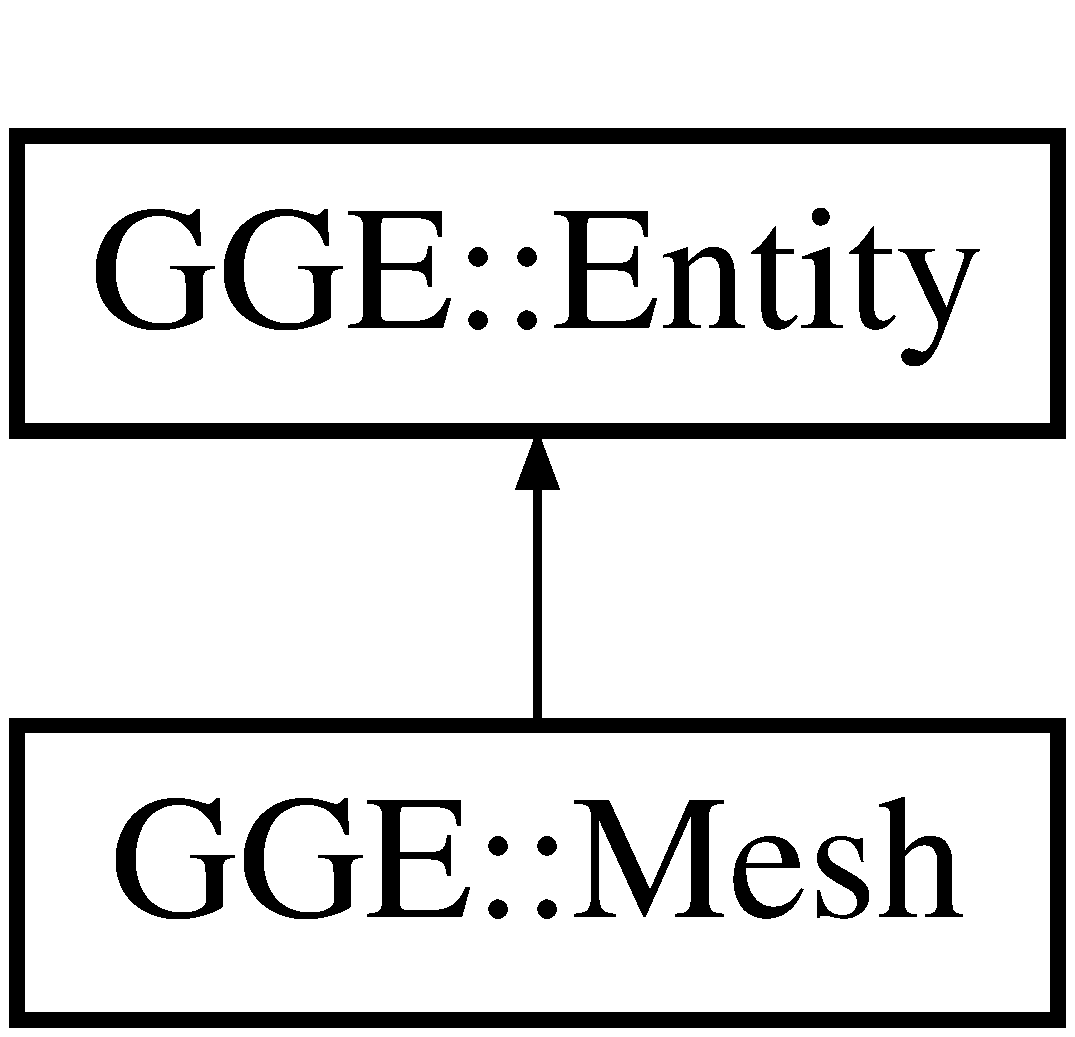
\includegraphics[height=2.000000cm]{class_g_g_e_1_1_mesh}
\end{center}
\end{figure}
\subsection*{Public Member Functions}
\begin{DoxyCompactItemize}
\item 
\hyperlink{class_g_g_e_1_1_mesh_af2227f54556d5bae2cdaa84a44e4c890}{Mesh} (std\+::vector$<$ G\+Lfloat $>$ \hyperlink{class_g_g_e_1_1_mesh_ab91ef29f57f9f8b7cddb7f360da63f47}{points}, std\+::vector$<$ G\+Lfloat $>$ \hyperlink{class_g_g_e_1_1_mesh_a7e48e26708078727065dd68e58846503}{texture\+Coords}, \hyperlink{class_g_g_e_1_1_texture}{Texture} $\ast$\hyperlink{class_g_g_e_1_1_mesh_acda1261106fd88be1bfc6a9adaa0e7b5}{texture}, \hyperlink{class_g_g_e_1_1_program}{Program} $\ast$\hyperlink{class_g_g_e_1_1_mesh_aee3bd238788ee7380e8d6770d5f29f2c}{program}, G\+Lenum \hyperlink{class_g_g_e_1_1_mesh_a92c516168dc3400a468cd4dd632287f6}{draw\+Type}=G\+L\+\_\+\+S\+T\+A\+T\+I\+C\+\_\+\+D\+R\+A\+W, G\+Lenum \hyperlink{class_g_g_e_1_1_mesh_a31f188bc943c5586befddc8838bd7c9a}{draw\+Shape}=G\+L\+\_\+\+T\+R\+I\+A\+N\+G\+L\+E\+S)
\item 
\hyperlink{class_g_g_e_1_1_mesh_a4a5408368fd4e8432b6c079432d4d039}{Mesh} (std\+::vector$<$ G\+Lfloat $>$ \hyperlink{class_g_g_e_1_1_mesh_ab91ef29f57f9f8b7cddb7f360da63f47}{points})
\item 
\hyperlink{class_g_g_e_1_1_mesh_a7c3fcda3195e1a67089bd9866d50aae7}{Mesh} (const char $\ast$filename, const char $\ast$directory, \hyperlink{class_g_g_e_1_1_program}{Program} $\ast$\hyperlink{class_g_g_e_1_1_mesh_aee3bd238788ee7380e8d6770d5f29f2c}{program})
\item 
\hyperlink{class_g_g_e_1_1_mesh_a33c847d16eaa0c19ee23d452d51ada24}{$\sim$\+Mesh} ()
\item 
void \hyperlink{class_g_g_e_1_1_mesh_af3ea4a760ffcd84cbb428f859f74778e}{draw} ()
\item 
glm\+::mat4 \hyperlink{class_g_g_e_1_1_mesh_a01cf6257386d96ba81ac1f80c650f0bd}{get\+Model\+Matrix} ()
\item 
glm\+::vec3 \hyperlink{class_g_g_e_1_1_mesh_a40161efa046c5513710bae8db2848d20}{move} (glm\+::vec3 translation)
\item 
glm\+::vec3 \hyperlink{class_g_g_e_1_1_mesh_a96e3bdea0c48b75b858261e0a6ac1eb6}{set\+Position} (glm\+::vec3 new\+Position)
\end{DoxyCompactItemize}
\subsection*{Private Member Functions}
\begin{DoxyCompactItemize}
\item 
void \hyperlink{class_g_g_e_1_1_mesh_aed1ab1e99e0a433d92f3c63db5401853}{init} ()
\end{DoxyCompactItemize}
\subsection*{Private Attributes}
\begin{DoxyCompactItemize}
\item 
std\+::vector$<$ \hyperlink{class_g_g_e_1_1_shape}{Shape} $\ast$ $>$ \hyperlink{class_g_g_e_1_1_mesh_a47f9d96f13ba1a491de0bd3c3adb9a76}{shapes}
\item 
std\+::vector$<$ G\+Lfloat $>$ \hyperlink{class_g_g_e_1_1_mesh_ab91ef29f57f9f8b7cddb7f360da63f47}{points}
\item 
glm\+::mat4 \hyperlink{class_g_g_e_1_1_mesh_a8ec6ca9082c5573198be3e9d675c2e92}{model\+Matrix}
\item 
\hyperlink{class_g_g_e_1_1_texture}{Texture} $\ast$ \hyperlink{class_g_g_e_1_1_mesh_acda1261106fd88be1bfc6a9adaa0e7b5}{texture}
\item 
\hyperlink{class_g_g_e_1_1_program}{Program} $\ast$ \hyperlink{class_g_g_e_1_1_mesh_aee3bd238788ee7380e8d6770d5f29f2c}{program}
\item 
std\+::vector$<$ G\+Lfloat $>$ \hyperlink{class_g_g_e_1_1_mesh_a7e48e26708078727065dd68e58846503}{texture\+Coords}
\item 
G\+Luint \hyperlink{class_g_g_e_1_1_mesh_a547c5fcf688b6a957c3febd742d51f9f}{vao}
\item 
G\+Lenum \hyperlink{class_g_g_e_1_1_mesh_a92c516168dc3400a468cd4dd632287f6}{draw\+Type}
\item 
G\+Lenum \hyperlink{class_g_g_e_1_1_mesh_a31f188bc943c5586befddc8838bd7c9a}{draw\+Shape}
\end{DoxyCompactItemize}
\subsection*{Additional Inherited Members}


\subsection{Constructor \& Destructor Documentation}
\hypertarget{class_g_g_e_1_1_mesh_af2227f54556d5bae2cdaa84a44e4c890}{\index{G\+G\+E\+::\+Mesh@{G\+G\+E\+::\+Mesh}!Mesh@{Mesh}}
\index{Mesh@{Mesh}!G\+G\+E\+::\+Mesh@{G\+G\+E\+::\+Mesh}}
\subsubsection[{Mesh}]{\setlength{\rightskip}{0pt plus 5cm}G\+G\+E\+::\+Mesh\+::\+Mesh (
\begin{DoxyParamCaption}
\item[{std\+::vector$<$ G\+Lfloat $>$}]{points, }
\item[{std\+::vector$<$ G\+Lfloat $>$}]{texture\+Coords, }
\item[{{\bf Texture} $\ast$}]{texture, }
\item[{{\bf Program} $\ast$}]{program, }
\item[{G\+Lenum}]{draw\+Type = {\ttfamily GL\+\_\+STATIC\+\_\+DRAW}, }
\item[{G\+Lenum}]{draw\+Shape = {\ttfamily GL\+\_\+TRIANGLES}}
\end{DoxyParamCaption}
)}}\label{class_g_g_e_1_1_mesh_af2227f54556d5bae2cdaa84a44e4c890}
\hypertarget{class_g_g_e_1_1_mesh_a4a5408368fd4e8432b6c079432d4d039}{\index{G\+G\+E\+::\+Mesh@{G\+G\+E\+::\+Mesh}!Mesh@{Mesh}}
\index{Mesh@{Mesh}!G\+G\+E\+::\+Mesh@{G\+G\+E\+::\+Mesh}}
\subsubsection[{Mesh}]{\setlength{\rightskip}{0pt plus 5cm}G\+G\+E\+::\+Mesh\+::\+Mesh (
\begin{DoxyParamCaption}
\item[{std\+::vector$<$ G\+Lfloat $>$}]{points}
\end{DoxyParamCaption}
)}}\label{class_g_g_e_1_1_mesh_a4a5408368fd4e8432b6c079432d4d039}
\hypertarget{class_g_g_e_1_1_mesh_a7c3fcda3195e1a67089bd9866d50aae7}{\index{G\+G\+E\+::\+Mesh@{G\+G\+E\+::\+Mesh}!Mesh@{Mesh}}
\index{Mesh@{Mesh}!G\+G\+E\+::\+Mesh@{G\+G\+E\+::\+Mesh}}
\subsubsection[{Mesh}]{\setlength{\rightskip}{0pt plus 5cm}G\+G\+E\+::\+Mesh\+::\+Mesh (
\begin{DoxyParamCaption}
\item[{const char $\ast$}]{filename, }
\item[{const char $\ast$}]{directory, }
\item[{{\bf Program} $\ast$}]{program}
\end{DoxyParamCaption}
)}}\label{class_g_g_e_1_1_mesh_a7c3fcda3195e1a67089bd9866d50aae7}
\hypertarget{class_g_g_e_1_1_mesh_a33c847d16eaa0c19ee23d452d51ada24}{\index{G\+G\+E\+::\+Mesh@{G\+G\+E\+::\+Mesh}!````~Mesh@{$\sim$\+Mesh}}
\index{````~Mesh@{$\sim$\+Mesh}!G\+G\+E\+::\+Mesh@{G\+G\+E\+::\+Mesh}}
\subsubsection[{$\sim$\+Mesh}]{\setlength{\rightskip}{0pt plus 5cm}G\+G\+E\+::\+Mesh\+::$\sim$\+Mesh (
\begin{DoxyParamCaption}
{}
\end{DoxyParamCaption}
)}}\label{class_g_g_e_1_1_mesh_a33c847d16eaa0c19ee23d452d51ada24}


\subsection{Member Function Documentation}
\hypertarget{class_g_g_e_1_1_mesh_af3ea4a760ffcd84cbb428f859f74778e}{\index{G\+G\+E\+::\+Mesh@{G\+G\+E\+::\+Mesh}!draw@{draw}}
\index{draw@{draw}!G\+G\+E\+::\+Mesh@{G\+G\+E\+::\+Mesh}}
\subsubsection[{draw}]{\setlength{\rightskip}{0pt plus 5cm}void G\+G\+E\+::\+Mesh\+::draw (
\begin{DoxyParamCaption}
{}
\end{DoxyParamCaption}
)}}\label{class_g_g_e_1_1_mesh_af3ea4a760ffcd84cbb428f859f74778e}
\hypertarget{class_g_g_e_1_1_mesh_a01cf6257386d96ba81ac1f80c650f0bd}{\index{G\+G\+E\+::\+Mesh@{G\+G\+E\+::\+Mesh}!get\+Model\+Matrix@{get\+Model\+Matrix}}
\index{get\+Model\+Matrix@{get\+Model\+Matrix}!G\+G\+E\+::\+Mesh@{G\+G\+E\+::\+Mesh}}
\subsubsection[{get\+Model\+Matrix}]{\setlength{\rightskip}{0pt plus 5cm}glm\+::mat4 G\+G\+E\+::\+Mesh\+::get\+Model\+Matrix (
\begin{DoxyParamCaption}
{}
\end{DoxyParamCaption}
)}}\label{class_g_g_e_1_1_mesh_a01cf6257386d96ba81ac1f80c650f0bd}
\hypertarget{class_g_g_e_1_1_mesh_aed1ab1e99e0a433d92f3c63db5401853}{\index{G\+G\+E\+::\+Mesh@{G\+G\+E\+::\+Mesh}!init@{init}}
\index{init@{init}!G\+G\+E\+::\+Mesh@{G\+G\+E\+::\+Mesh}}
\subsubsection[{init}]{\setlength{\rightskip}{0pt plus 5cm}void G\+G\+E\+::\+Mesh\+::init (
\begin{DoxyParamCaption}
{}
\end{DoxyParamCaption}
)\hspace{0.3cm}{\ttfamily [private]}}}\label{class_g_g_e_1_1_mesh_aed1ab1e99e0a433d92f3c63db5401853}
\hypertarget{class_g_g_e_1_1_mesh_a40161efa046c5513710bae8db2848d20}{\index{G\+G\+E\+::\+Mesh@{G\+G\+E\+::\+Mesh}!move@{move}}
\index{move@{move}!G\+G\+E\+::\+Mesh@{G\+G\+E\+::\+Mesh}}
\subsubsection[{move}]{\setlength{\rightskip}{0pt plus 5cm}glm\+::vec3 G\+G\+E\+::\+Mesh\+::move (
\begin{DoxyParamCaption}
\item[{glm\+::vec3}]{translation}
\end{DoxyParamCaption}
)\hspace{0.3cm}{\ttfamily [virtual]}}}\label{class_g_g_e_1_1_mesh_a40161efa046c5513710bae8db2848d20}


Reimplemented from \hyperlink{class_g_g_e_1_1_entity_a7525dd307ec84c0eb4052886142a57fb}{G\+G\+E\+::\+Entity}.

\hypertarget{class_g_g_e_1_1_mesh_a96e3bdea0c48b75b858261e0a6ac1eb6}{\index{G\+G\+E\+::\+Mesh@{G\+G\+E\+::\+Mesh}!set\+Position@{set\+Position}}
\index{set\+Position@{set\+Position}!G\+G\+E\+::\+Mesh@{G\+G\+E\+::\+Mesh}}
\subsubsection[{set\+Position}]{\setlength{\rightskip}{0pt plus 5cm}glm\+::vec3 G\+G\+E\+::\+Mesh\+::set\+Position (
\begin{DoxyParamCaption}
\item[{glm\+::vec3}]{new\+Position}
\end{DoxyParamCaption}
)\hspace{0.3cm}{\ttfamily [virtual]}}}\label{class_g_g_e_1_1_mesh_a96e3bdea0c48b75b858261e0a6ac1eb6}


Reimplemented from \hyperlink{class_g_g_e_1_1_entity_a2281d937a3430a14ec23b9a10b91efcb}{G\+G\+E\+::\+Entity}.



\subsection{Member Data Documentation}
\hypertarget{class_g_g_e_1_1_mesh_a31f188bc943c5586befddc8838bd7c9a}{\index{G\+G\+E\+::\+Mesh@{G\+G\+E\+::\+Mesh}!draw\+Shape@{draw\+Shape}}
\index{draw\+Shape@{draw\+Shape}!G\+G\+E\+::\+Mesh@{G\+G\+E\+::\+Mesh}}
\subsubsection[{draw\+Shape}]{\setlength{\rightskip}{0pt plus 5cm}G\+Lenum G\+G\+E\+::\+Mesh\+::draw\+Shape\hspace{0.3cm}{\ttfamily [private]}}}\label{class_g_g_e_1_1_mesh_a31f188bc943c5586befddc8838bd7c9a}
\hypertarget{class_g_g_e_1_1_mesh_a92c516168dc3400a468cd4dd632287f6}{\index{G\+G\+E\+::\+Mesh@{G\+G\+E\+::\+Mesh}!draw\+Type@{draw\+Type}}
\index{draw\+Type@{draw\+Type}!G\+G\+E\+::\+Mesh@{G\+G\+E\+::\+Mesh}}
\subsubsection[{draw\+Type}]{\setlength{\rightskip}{0pt plus 5cm}G\+Lenum G\+G\+E\+::\+Mesh\+::draw\+Type\hspace{0.3cm}{\ttfamily [private]}}}\label{class_g_g_e_1_1_mesh_a92c516168dc3400a468cd4dd632287f6}
\hypertarget{class_g_g_e_1_1_mesh_a8ec6ca9082c5573198be3e9d675c2e92}{\index{G\+G\+E\+::\+Mesh@{G\+G\+E\+::\+Mesh}!model\+Matrix@{model\+Matrix}}
\index{model\+Matrix@{model\+Matrix}!G\+G\+E\+::\+Mesh@{G\+G\+E\+::\+Mesh}}
\subsubsection[{model\+Matrix}]{\setlength{\rightskip}{0pt plus 5cm}glm\+::mat4 G\+G\+E\+::\+Mesh\+::model\+Matrix\hspace{0.3cm}{\ttfamily [private]}}}\label{class_g_g_e_1_1_mesh_a8ec6ca9082c5573198be3e9d675c2e92}
\hypertarget{class_g_g_e_1_1_mesh_ab91ef29f57f9f8b7cddb7f360da63f47}{\index{G\+G\+E\+::\+Mesh@{G\+G\+E\+::\+Mesh}!points@{points}}
\index{points@{points}!G\+G\+E\+::\+Mesh@{G\+G\+E\+::\+Mesh}}
\subsubsection[{points}]{\setlength{\rightskip}{0pt plus 5cm}std\+::vector$<$G\+Lfloat$>$ G\+G\+E\+::\+Mesh\+::points\hspace{0.3cm}{\ttfamily [private]}}}\label{class_g_g_e_1_1_mesh_ab91ef29f57f9f8b7cddb7f360da63f47}
\hypertarget{class_g_g_e_1_1_mesh_aee3bd238788ee7380e8d6770d5f29f2c}{\index{G\+G\+E\+::\+Mesh@{G\+G\+E\+::\+Mesh}!program@{program}}
\index{program@{program}!G\+G\+E\+::\+Mesh@{G\+G\+E\+::\+Mesh}}
\subsubsection[{program}]{\setlength{\rightskip}{0pt plus 5cm}{\bf Program}$\ast$ G\+G\+E\+::\+Mesh\+::program\hspace{0.3cm}{\ttfamily [private]}}}\label{class_g_g_e_1_1_mesh_aee3bd238788ee7380e8d6770d5f29f2c}
\hypertarget{class_g_g_e_1_1_mesh_a47f9d96f13ba1a491de0bd3c3adb9a76}{\index{G\+G\+E\+::\+Mesh@{G\+G\+E\+::\+Mesh}!shapes@{shapes}}
\index{shapes@{shapes}!G\+G\+E\+::\+Mesh@{G\+G\+E\+::\+Mesh}}
\subsubsection[{shapes}]{\setlength{\rightskip}{0pt plus 5cm}std\+::vector$<${\bf Shape} $\ast$$>$ G\+G\+E\+::\+Mesh\+::shapes\hspace{0.3cm}{\ttfamily [private]}}}\label{class_g_g_e_1_1_mesh_a47f9d96f13ba1a491de0bd3c3adb9a76}
\hypertarget{class_g_g_e_1_1_mesh_acda1261106fd88be1bfc6a9adaa0e7b5}{\index{G\+G\+E\+::\+Mesh@{G\+G\+E\+::\+Mesh}!texture@{texture}}
\index{texture@{texture}!G\+G\+E\+::\+Mesh@{G\+G\+E\+::\+Mesh}}
\subsubsection[{texture}]{\setlength{\rightskip}{0pt plus 5cm}{\bf Texture}$\ast$ G\+G\+E\+::\+Mesh\+::texture\hspace{0.3cm}{\ttfamily [private]}}}\label{class_g_g_e_1_1_mesh_acda1261106fd88be1bfc6a9adaa0e7b5}
\hypertarget{class_g_g_e_1_1_mesh_a7e48e26708078727065dd68e58846503}{\index{G\+G\+E\+::\+Mesh@{G\+G\+E\+::\+Mesh}!texture\+Coords@{texture\+Coords}}
\index{texture\+Coords@{texture\+Coords}!G\+G\+E\+::\+Mesh@{G\+G\+E\+::\+Mesh}}
\subsubsection[{texture\+Coords}]{\setlength{\rightskip}{0pt plus 5cm}std\+::vector$<$G\+Lfloat$>$ G\+G\+E\+::\+Mesh\+::texture\+Coords\hspace{0.3cm}{\ttfamily [private]}}}\label{class_g_g_e_1_1_mesh_a7e48e26708078727065dd68e58846503}
\hypertarget{class_g_g_e_1_1_mesh_a547c5fcf688b6a957c3febd742d51f9f}{\index{G\+G\+E\+::\+Mesh@{G\+G\+E\+::\+Mesh}!vao@{vao}}
\index{vao@{vao}!G\+G\+E\+::\+Mesh@{G\+G\+E\+::\+Mesh}}
\subsubsection[{vao}]{\setlength{\rightskip}{0pt plus 5cm}G\+Luint G\+G\+E\+::\+Mesh\+::vao\hspace{0.3cm}{\ttfamily [private]}}}\label{class_g_g_e_1_1_mesh_a547c5fcf688b6a957c3febd742d51f9f}


The documentation for this class was generated from the following files\+:\begin{DoxyCompactItemize}
\item 
include/\hyperlink{mesh_8h}{mesh.\+h}\item 
src/\hyperlink{mesh_8cpp}{mesh.\+cpp}\end{DoxyCompactItemize}

\hypertarget{class_g_g_e_1_1_point_light}{\section{G\+G\+E\+:\+:Point\+Light Class Reference}
\label{class_g_g_e_1_1_point_light}\index{G\+G\+E\+::\+Point\+Light@{G\+G\+E\+::\+Point\+Light}}
}


{\ttfamily \#include $<$light.\+h$>$}

Inheritance diagram for G\+G\+E\+:\+:Point\+Light\+:\begin{figure}[H]
\begin{center}
\leavevmode
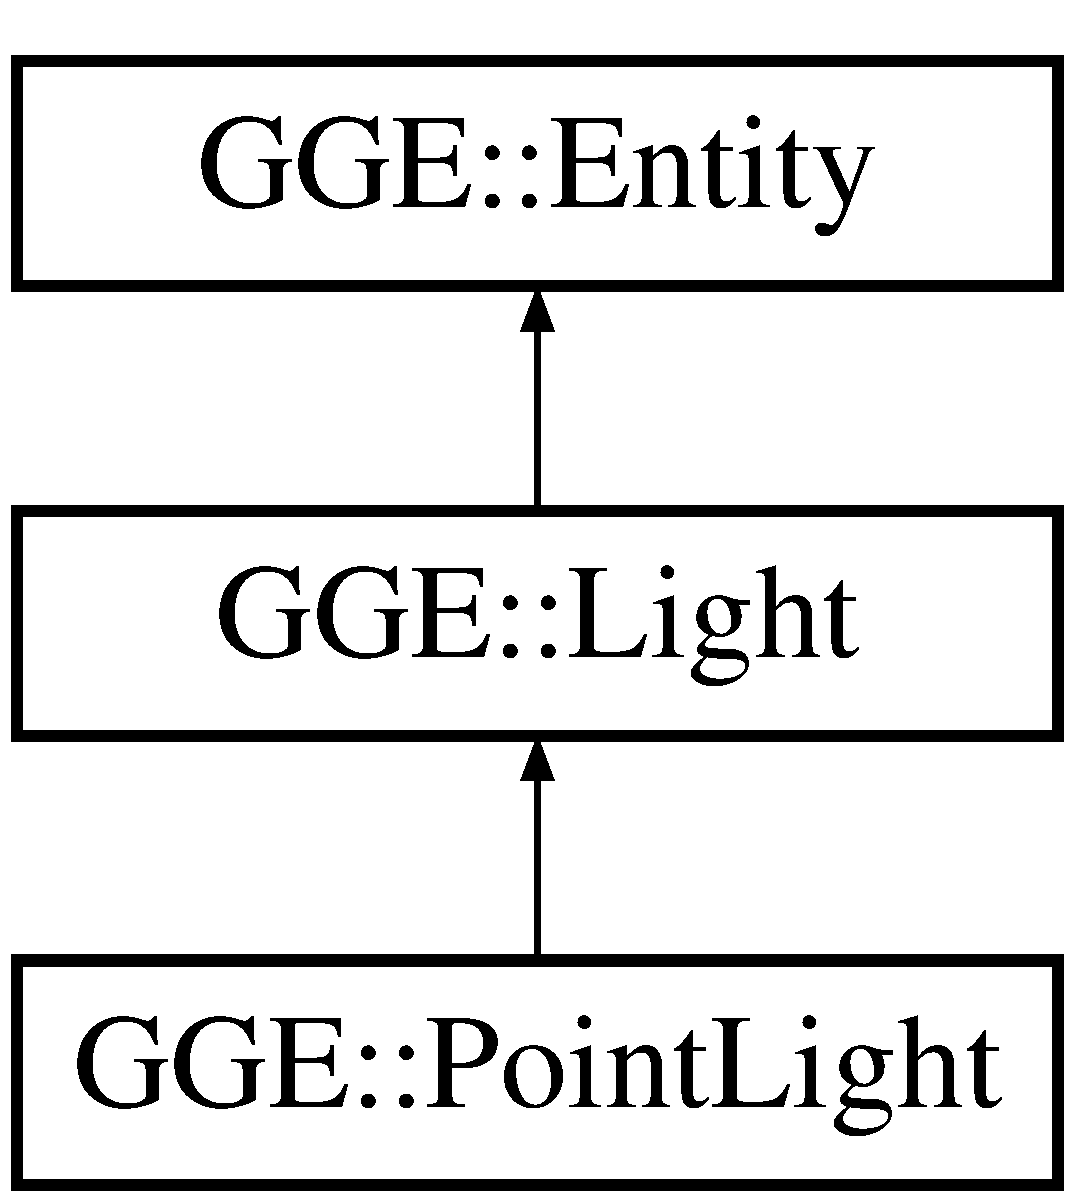
\includegraphics[height=3.000000cm]{class_g_g_e_1_1_point_light}
\end{center}
\end{figure}
\subsection*{Public Member Functions}
\begin{DoxyCompactItemize}
\item 
\hyperlink{class_g_g_e_1_1_point_light_a57e66c237c2a361f155aafec8dc11e5f}{Point\+Light} (glm\+::vec3 \hyperlink{class_g_g_e_1_1_entity_a38a9fa01bfaf37ca415181ba6a179d3f}{position}, glm\+::vec3 \hyperlink{class_g_g_e_1_1_entity_a80c69365314541244f26e4a15b4223d8}{direction}, \hyperlink{namespace_g_g_e_aff43741fd756c83cbfd5d4d5cd9fcf41}{Color4} \hyperlink{class_g_g_e_1_1_light_a4d2f4605abc44637feac0d0312ce0717}{color})
\item 
\hyperlink{class_g_g_e_1_1_point_light_a82fa83bf3fa1a70b04745d5710d964a8}{$\sim$\+Point\+Light} ()
\end{DoxyCompactItemize}
\subsection*{Additional Inherited Members}


\subsection{Constructor \& Destructor Documentation}
\hypertarget{class_g_g_e_1_1_point_light_a57e66c237c2a361f155aafec8dc11e5f}{\index{G\+G\+E\+::\+Point\+Light@{G\+G\+E\+::\+Point\+Light}!Point\+Light@{Point\+Light}}
\index{Point\+Light@{Point\+Light}!G\+G\+E\+::\+Point\+Light@{G\+G\+E\+::\+Point\+Light}}
\subsubsection[{Point\+Light}]{\setlength{\rightskip}{0pt plus 5cm}G\+G\+E\+::\+Point\+Light\+::\+Point\+Light (
\begin{DoxyParamCaption}
\item[{glm\+::vec3}]{position, }
\item[{glm\+::vec3}]{direction, }
\item[{{\bf Color4}}]{color}
\end{DoxyParamCaption}
)}}\label{class_g_g_e_1_1_point_light_a57e66c237c2a361f155aafec8dc11e5f}
\hypertarget{class_g_g_e_1_1_point_light_a82fa83bf3fa1a70b04745d5710d964a8}{\index{G\+G\+E\+::\+Point\+Light@{G\+G\+E\+::\+Point\+Light}!````~Point\+Light@{$\sim$\+Point\+Light}}
\index{````~Point\+Light@{$\sim$\+Point\+Light}!G\+G\+E\+::\+Point\+Light@{G\+G\+E\+::\+Point\+Light}}
\subsubsection[{$\sim$\+Point\+Light}]{\setlength{\rightskip}{0pt plus 5cm}G\+G\+E\+::\+Point\+Light\+::$\sim$\+Point\+Light (
\begin{DoxyParamCaption}
{}
\end{DoxyParamCaption}
)}}\label{class_g_g_e_1_1_point_light_a82fa83bf3fa1a70b04745d5710d964a8}


The documentation for this class was generated from the following files\+:\begin{DoxyCompactItemize}
\item 
include/\hyperlink{light_8h}{light.\+h}\item 
src/\hyperlink{light_8cpp}{light.\+cpp}\end{DoxyCompactItemize}

\hypertarget{class_g_g_e_1_1_program}{\section{G\+G\+E\+:\+:Program Class Reference}
\label{class_g_g_e_1_1_program}\index{G\+G\+E\+::\+Program@{G\+G\+E\+::\+Program}}
}


{\ttfamily \#include $<$program.\+h$>$}

\subsection*{Public Member Functions}
\begin{DoxyCompactItemize}
\item 
\hyperlink{class_g_g_e_1_1_program_a3879f737244244d8689b2708de63c55f}{Program} (std\+::vector$<$ \hyperlink{class_g_g_e_1_1_shader}{Shader} $\ast$ $>$ \hyperlink{class_g_g_e_1_1_program_a6f31b509c852f7271282d5ad79056b18}{shaders})
\item 
\hyperlink{class_g_g_e_1_1_program_aab1fc451cf7e926bf4bb9f8c99d904ed}{$\sim$\+Program} ()
\item 
G\+Luint \hyperlink{class_g_g_e_1_1_program_aeb2aa9fb22fd5ce5d6d981d3308ec576}{get\+Program\+I\+D} ()
\item 
G\+Luint \hyperlink{class_g_g_e_1_1_program_ab8444f45bd2a41920a41e84d2023d2d1}{bind} ()
\item 
G\+Luint \hyperlink{class_g_g_e_1_1_program_ab703c352644e33680907edfde5140654}{unbind} ()
\item 
G\+Luint \hyperlink{class_g_g_e_1_1_program_aec23fac66944617abdb3beb82b8886a0}{get\+Attrib} (const G\+Lchar $\ast$attrib\+Name)
\item 
G\+Luint \hyperlink{class_g_g_e_1_1_program_af1d316e47de393df33d9f6e58292fbdb}{get\+Uniform} (const G\+Lchar $\ast$uniform\+Name)
\end{DoxyCompactItemize}
\subsection*{Static Public Member Functions}
\begin{DoxyCompactItemize}
\item 
static \hyperlink{class_g_g_e_1_1_program}{Program} $\ast$ \hyperlink{class_g_g_e_1_1_program_a37badf65e989bee6d3dc3842ae0b5ccf}{get\+Current\+Program} ()
\item 
static void \hyperlink{class_g_g_e_1_1_program_a5e1fa577efd1cd96531b2a0a8e497423}{update\+Projection\+Matrix} (glm\+::mat4 projection\+Matrix)
\item 
static void \hyperlink{class_g_g_e_1_1_program_a2ad116e144ea1c29b33a6d28e0ff1447}{update\+View\+Matrix} (glm\+::mat4 view\+Matrix)
\end{DoxyCompactItemize}
\subsection*{Private Attributes}
\begin{DoxyCompactItemize}
\item 
G\+Luint \hyperlink{class_g_g_e_1_1_program_aa011e6183ba2be3e3d99d9e03101fb3d}{program\+I\+D}
\item 
std\+::vector$<$ \hyperlink{class_g_g_e_1_1_shader}{Shader} $\ast$ $>$ \hyperlink{class_g_g_e_1_1_program_a6f31b509c852f7271282d5ad79056b18}{shaders}
\end{DoxyCompactItemize}
\subsection*{Static Private Attributes}
\begin{DoxyCompactItemize}
\item 
static \hyperlink{class_g_g_e_1_1_program}{Program} $\ast$ \hyperlink{class_g_g_e_1_1_program_a006a547745798242ceb402b9e5a1ed1b}{current\+Program} = N\+U\+L\+L
\item 
static std\+::list$<$ \hyperlink{class_g_g_e_1_1_program}{Program} $\ast$ $>$ \hyperlink{class_g_g_e_1_1_program_ac6342a249c1333e4364bf8e4ac0d9b39}{active\+Programs}
\end{DoxyCompactItemize}


\subsection{Constructor \& Destructor Documentation}
\hypertarget{class_g_g_e_1_1_program_a3879f737244244d8689b2708de63c55f}{\index{G\+G\+E\+::\+Program@{G\+G\+E\+::\+Program}!Program@{Program}}
\index{Program@{Program}!G\+G\+E\+::\+Program@{G\+G\+E\+::\+Program}}
\subsubsection[{Program}]{\setlength{\rightskip}{0pt plus 5cm}G\+G\+E\+::\+Program\+::\+Program (
\begin{DoxyParamCaption}
\item[{std\+::vector$<$ {\bf Shader} $\ast$ $>$}]{shaders}
\end{DoxyParamCaption}
)}}\label{class_g_g_e_1_1_program_a3879f737244244d8689b2708de63c55f}
\hypertarget{class_g_g_e_1_1_program_aab1fc451cf7e926bf4bb9f8c99d904ed}{\index{G\+G\+E\+::\+Program@{G\+G\+E\+::\+Program}!````~Program@{$\sim$\+Program}}
\index{````~Program@{$\sim$\+Program}!G\+G\+E\+::\+Program@{G\+G\+E\+::\+Program}}
\subsubsection[{$\sim$\+Program}]{\setlength{\rightskip}{0pt plus 5cm}G\+G\+E\+::\+Program\+::$\sim$\+Program (
\begin{DoxyParamCaption}
{}
\end{DoxyParamCaption}
)}}\label{class_g_g_e_1_1_program_aab1fc451cf7e926bf4bb9f8c99d904ed}


\subsection{Member Function Documentation}
\hypertarget{class_g_g_e_1_1_program_ab8444f45bd2a41920a41e84d2023d2d1}{\index{G\+G\+E\+::\+Program@{G\+G\+E\+::\+Program}!bind@{bind}}
\index{bind@{bind}!G\+G\+E\+::\+Program@{G\+G\+E\+::\+Program}}
\subsubsection[{bind}]{\setlength{\rightskip}{0pt plus 5cm}G\+Luint G\+G\+E\+::\+Program\+::bind (
\begin{DoxyParamCaption}
{}
\end{DoxyParamCaption}
)}}\label{class_g_g_e_1_1_program_ab8444f45bd2a41920a41e84d2023d2d1}
\hypertarget{class_g_g_e_1_1_program_aec23fac66944617abdb3beb82b8886a0}{\index{G\+G\+E\+::\+Program@{G\+G\+E\+::\+Program}!get\+Attrib@{get\+Attrib}}
\index{get\+Attrib@{get\+Attrib}!G\+G\+E\+::\+Program@{G\+G\+E\+::\+Program}}
\subsubsection[{get\+Attrib}]{\setlength{\rightskip}{0pt plus 5cm}G\+Luint G\+G\+E\+::\+Program\+::get\+Attrib (
\begin{DoxyParamCaption}
\item[{const G\+Lchar $\ast$}]{attrib\+Name}
\end{DoxyParamCaption}
)}}\label{class_g_g_e_1_1_program_aec23fac66944617abdb3beb82b8886a0}
\hypertarget{class_g_g_e_1_1_program_a37badf65e989bee6d3dc3842ae0b5ccf}{\index{G\+G\+E\+::\+Program@{G\+G\+E\+::\+Program}!get\+Current\+Program@{get\+Current\+Program}}
\index{get\+Current\+Program@{get\+Current\+Program}!G\+G\+E\+::\+Program@{G\+G\+E\+::\+Program}}
\subsubsection[{get\+Current\+Program}]{\setlength{\rightskip}{0pt plus 5cm}{\bf Program} $\ast$ G\+G\+E\+::\+Program\+::get\+Current\+Program (
\begin{DoxyParamCaption}
{}
\end{DoxyParamCaption}
)\hspace{0.3cm}{\ttfamily [static]}}}\label{class_g_g_e_1_1_program_a37badf65e989bee6d3dc3842ae0b5ccf}
\hypertarget{class_g_g_e_1_1_program_aeb2aa9fb22fd5ce5d6d981d3308ec576}{\index{G\+G\+E\+::\+Program@{G\+G\+E\+::\+Program}!get\+Program\+I\+D@{get\+Program\+I\+D}}
\index{get\+Program\+I\+D@{get\+Program\+I\+D}!G\+G\+E\+::\+Program@{G\+G\+E\+::\+Program}}
\subsubsection[{get\+Program\+I\+D}]{\setlength{\rightskip}{0pt plus 5cm}G\+Luint G\+G\+E\+::\+Program\+::get\+Program\+I\+D (
\begin{DoxyParamCaption}
{}
\end{DoxyParamCaption}
)}}\label{class_g_g_e_1_1_program_aeb2aa9fb22fd5ce5d6d981d3308ec576}
\hypertarget{class_g_g_e_1_1_program_af1d316e47de393df33d9f6e58292fbdb}{\index{G\+G\+E\+::\+Program@{G\+G\+E\+::\+Program}!get\+Uniform@{get\+Uniform}}
\index{get\+Uniform@{get\+Uniform}!G\+G\+E\+::\+Program@{G\+G\+E\+::\+Program}}
\subsubsection[{get\+Uniform}]{\setlength{\rightskip}{0pt plus 5cm}G\+Luint G\+G\+E\+::\+Program\+::get\+Uniform (
\begin{DoxyParamCaption}
\item[{const G\+Lchar $\ast$}]{uniform\+Name}
\end{DoxyParamCaption}
)}}\label{class_g_g_e_1_1_program_af1d316e47de393df33d9f6e58292fbdb}
\hypertarget{class_g_g_e_1_1_program_ab703c352644e33680907edfde5140654}{\index{G\+G\+E\+::\+Program@{G\+G\+E\+::\+Program}!unbind@{unbind}}
\index{unbind@{unbind}!G\+G\+E\+::\+Program@{G\+G\+E\+::\+Program}}
\subsubsection[{unbind}]{\setlength{\rightskip}{0pt plus 5cm}G\+Luint G\+G\+E\+::\+Program\+::unbind (
\begin{DoxyParamCaption}
{}
\end{DoxyParamCaption}
)}}\label{class_g_g_e_1_1_program_ab703c352644e33680907edfde5140654}
\hypertarget{class_g_g_e_1_1_program_a5e1fa577efd1cd96531b2a0a8e497423}{\index{G\+G\+E\+::\+Program@{G\+G\+E\+::\+Program}!update\+Projection\+Matrix@{update\+Projection\+Matrix}}
\index{update\+Projection\+Matrix@{update\+Projection\+Matrix}!G\+G\+E\+::\+Program@{G\+G\+E\+::\+Program}}
\subsubsection[{update\+Projection\+Matrix}]{\setlength{\rightskip}{0pt plus 5cm}void G\+G\+E\+::\+Program\+::update\+Projection\+Matrix (
\begin{DoxyParamCaption}
\item[{glm\+::mat4}]{projection\+Matrix}
\end{DoxyParamCaption}
)\hspace{0.3cm}{\ttfamily [static]}}}\label{class_g_g_e_1_1_program_a5e1fa577efd1cd96531b2a0a8e497423}
\hypertarget{class_g_g_e_1_1_program_a2ad116e144ea1c29b33a6d28e0ff1447}{\index{G\+G\+E\+::\+Program@{G\+G\+E\+::\+Program}!update\+View\+Matrix@{update\+View\+Matrix}}
\index{update\+View\+Matrix@{update\+View\+Matrix}!G\+G\+E\+::\+Program@{G\+G\+E\+::\+Program}}
\subsubsection[{update\+View\+Matrix}]{\setlength{\rightskip}{0pt plus 5cm}void G\+G\+E\+::\+Program\+::update\+View\+Matrix (
\begin{DoxyParamCaption}
\item[{glm\+::mat4}]{view\+Matrix}
\end{DoxyParamCaption}
)\hspace{0.3cm}{\ttfamily [static]}}}\label{class_g_g_e_1_1_program_a2ad116e144ea1c29b33a6d28e0ff1447}


\subsection{Member Data Documentation}
\hypertarget{class_g_g_e_1_1_program_ac6342a249c1333e4364bf8e4ac0d9b39}{\index{G\+G\+E\+::\+Program@{G\+G\+E\+::\+Program}!active\+Programs@{active\+Programs}}
\index{active\+Programs@{active\+Programs}!G\+G\+E\+::\+Program@{G\+G\+E\+::\+Program}}
\subsubsection[{active\+Programs}]{\setlength{\rightskip}{0pt plus 5cm}std\+::list$<$ {\bf Program} $\ast$ $>$ G\+G\+E\+::\+Program\+::active\+Programs\hspace{0.3cm}{\ttfamily [static]}, {\ttfamily [private]}}}\label{class_g_g_e_1_1_program_ac6342a249c1333e4364bf8e4ac0d9b39}
\hypertarget{class_g_g_e_1_1_program_a006a547745798242ceb402b9e5a1ed1b}{\index{G\+G\+E\+::\+Program@{G\+G\+E\+::\+Program}!current\+Program@{current\+Program}}
\index{current\+Program@{current\+Program}!G\+G\+E\+::\+Program@{G\+G\+E\+::\+Program}}
\subsubsection[{current\+Program}]{\setlength{\rightskip}{0pt plus 5cm}{\bf Program} $\ast$ G\+G\+E\+::\+Program\+::current\+Program = N\+U\+L\+L\hspace{0.3cm}{\ttfamily [static]}, {\ttfamily [private]}}}\label{class_g_g_e_1_1_program_a006a547745798242ceb402b9e5a1ed1b}
\hypertarget{class_g_g_e_1_1_program_aa011e6183ba2be3e3d99d9e03101fb3d}{\index{G\+G\+E\+::\+Program@{G\+G\+E\+::\+Program}!program\+I\+D@{program\+I\+D}}
\index{program\+I\+D@{program\+I\+D}!G\+G\+E\+::\+Program@{G\+G\+E\+::\+Program}}
\subsubsection[{program\+I\+D}]{\setlength{\rightskip}{0pt plus 5cm}G\+Luint G\+G\+E\+::\+Program\+::program\+I\+D\hspace{0.3cm}{\ttfamily [private]}}}\label{class_g_g_e_1_1_program_aa011e6183ba2be3e3d99d9e03101fb3d}
\hypertarget{class_g_g_e_1_1_program_a6f31b509c852f7271282d5ad79056b18}{\index{G\+G\+E\+::\+Program@{G\+G\+E\+::\+Program}!shaders@{shaders}}
\index{shaders@{shaders}!G\+G\+E\+::\+Program@{G\+G\+E\+::\+Program}}
\subsubsection[{shaders}]{\setlength{\rightskip}{0pt plus 5cm}std\+::vector$<${\bf Shader} $\ast$$>$ G\+G\+E\+::\+Program\+::shaders\hspace{0.3cm}{\ttfamily [private]}}}\label{class_g_g_e_1_1_program_a6f31b509c852f7271282d5ad79056b18}


The documentation for this class was generated from the following files\+:\begin{DoxyCompactItemize}
\item 
include/\hyperlink{program_8h}{program.\+h}\item 
src/\hyperlink{program_8cpp}{program.\+cpp}\end{DoxyCompactItemize}

\hypertarget{class_g_g_e_1_1_shader}{\section{G\+G\+E\+:\+:Shader Class Reference}
\label{class_g_g_e_1_1_shader}\index{G\+G\+E\+::\+Shader@{G\+G\+E\+::\+Shader}}
}


{\ttfamily \#include $<$shader.\+h$>$}

\subsection*{Public Member Functions}
\begin{DoxyCompactItemize}
\item 
\hyperlink{class_g_g_e_1_1_shader_afb84a4ca449db00a0fcee2294968542d}{Shader} (const char $\ast$filename, G\+Lenum \hyperlink{class_g_g_e_1_1_shader_a26f6e14c6c17ad9272adfa507616f325}{shader\+Type})
\item 
\hyperlink{class_g_g_e_1_1_shader_a8dfaa9c632964ffb3a49bb11041efac3}{$\sim$\+Shader} ()
\item 
G\+Luint \hyperlink{class_g_g_e_1_1_shader_a9938d49d13cd8bfae14518bab7841290}{get\+Shader\+I\+D} ()
\end{DoxyCompactItemize}
\subsection*{Private Attributes}
\begin{DoxyCompactItemize}
\item 
std\+::string \hyperlink{class_g_g_e_1_1_shader_ad5e9d91f6cf959482b669d8fbf7712a4}{shader\+String}
\item 
G\+Luint \hyperlink{class_g_g_e_1_1_shader_a8ae56489b492426e188fecb1cc3eb679}{shader\+I\+D}
\item 
G\+Lenum \hyperlink{class_g_g_e_1_1_shader_a26f6e14c6c17ad9272adfa507616f325}{shader\+Type}
\end{DoxyCompactItemize}


\subsection{Constructor \& Destructor Documentation}
\hypertarget{class_g_g_e_1_1_shader_afb84a4ca449db00a0fcee2294968542d}{\index{G\+G\+E\+::\+Shader@{G\+G\+E\+::\+Shader}!Shader@{Shader}}
\index{Shader@{Shader}!G\+G\+E\+::\+Shader@{G\+G\+E\+::\+Shader}}
\subsubsection[{Shader}]{\setlength{\rightskip}{0pt plus 5cm}G\+G\+E\+::\+Shader\+::\+Shader (
\begin{DoxyParamCaption}
\item[{const char $\ast$}]{filename, }
\item[{G\+Lenum}]{shader\+Type}
\end{DoxyParamCaption}
)}}\label{class_g_g_e_1_1_shader_afb84a4ca449db00a0fcee2294968542d}
\hypertarget{class_g_g_e_1_1_shader_a8dfaa9c632964ffb3a49bb11041efac3}{\index{G\+G\+E\+::\+Shader@{G\+G\+E\+::\+Shader}!````~Shader@{$\sim$\+Shader}}
\index{````~Shader@{$\sim$\+Shader}!G\+G\+E\+::\+Shader@{G\+G\+E\+::\+Shader}}
\subsubsection[{$\sim$\+Shader}]{\setlength{\rightskip}{0pt plus 5cm}G\+G\+E\+::\+Shader\+::$\sim$\+Shader (
\begin{DoxyParamCaption}
{}
\end{DoxyParamCaption}
)}}\label{class_g_g_e_1_1_shader_a8dfaa9c632964ffb3a49bb11041efac3}


\subsection{Member Function Documentation}
\hypertarget{class_g_g_e_1_1_shader_a9938d49d13cd8bfae14518bab7841290}{\index{G\+G\+E\+::\+Shader@{G\+G\+E\+::\+Shader}!get\+Shader\+I\+D@{get\+Shader\+I\+D}}
\index{get\+Shader\+I\+D@{get\+Shader\+I\+D}!G\+G\+E\+::\+Shader@{G\+G\+E\+::\+Shader}}
\subsubsection[{get\+Shader\+I\+D}]{\setlength{\rightskip}{0pt plus 5cm}G\+Luint G\+G\+E\+::\+Shader\+::get\+Shader\+I\+D (
\begin{DoxyParamCaption}
{}
\end{DoxyParamCaption}
)}}\label{class_g_g_e_1_1_shader_a9938d49d13cd8bfae14518bab7841290}


\subsection{Member Data Documentation}
\hypertarget{class_g_g_e_1_1_shader_a8ae56489b492426e188fecb1cc3eb679}{\index{G\+G\+E\+::\+Shader@{G\+G\+E\+::\+Shader}!shader\+I\+D@{shader\+I\+D}}
\index{shader\+I\+D@{shader\+I\+D}!G\+G\+E\+::\+Shader@{G\+G\+E\+::\+Shader}}
\subsubsection[{shader\+I\+D}]{\setlength{\rightskip}{0pt plus 5cm}G\+Luint G\+G\+E\+::\+Shader\+::shader\+I\+D\hspace{0.3cm}{\ttfamily [private]}}}\label{class_g_g_e_1_1_shader_a8ae56489b492426e188fecb1cc3eb679}
\hypertarget{class_g_g_e_1_1_shader_ad5e9d91f6cf959482b669d8fbf7712a4}{\index{G\+G\+E\+::\+Shader@{G\+G\+E\+::\+Shader}!shader\+String@{shader\+String}}
\index{shader\+String@{shader\+String}!G\+G\+E\+::\+Shader@{G\+G\+E\+::\+Shader}}
\subsubsection[{shader\+String}]{\setlength{\rightskip}{0pt plus 5cm}std\+::string G\+G\+E\+::\+Shader\+::shader\+String\hspace{0.3cm}{\ttfamily [private]}}}\label{class_g_g_e_1_1_shader_ad5e9d91f6cf959482b669d8fbf7712a4}
\hypertarget{class_g_g_e_1_1_shader_a26f6e14c6c17ad9272adfa507616f325}{\index{G\+G\+E\+::\+Shader@{G\+G\+E\+::\+Shader}!shader\+Type@{shader\+Type}}
\index{shader\+Type@{shader\+Type}!G\+G\+E\+::\+Shader@{G\+G\+E\+::\+Shader}}
\subsubsection[{shader\+Type}]{\setlength{\rightskip}{0pt plus 5cm}G\+Lenum G\+G\+E\+::\+Shader\+::shader\+Type\hspace{0.3cm}{\ttfamily [private]}}}\label{class_g_g_e_1_1_shader_a26f6e14c6c17ad9272adfa507616f325}


The documentation for this class was generated from the following files\+:\begin{DoxyCompactItemize}
\item 
include/\hyperlink{shader_8h}{shader.\+h}\item 
src/\hyperlink{shader_8cpp}{shader.\+cpp}\end{DoxyCompactItemize}

\hypertarget{class_g_g_e_1_1_shape}{\section{G\+G\+E\+:\+:Shape Class Reference}
\label{class_g_g_e_1_1_shape}\index{G\+G\+E\+::\+Shape@{G\+G\+E\+::\+Shape}}
}


{\ttfamily \#include $<$shape.\+h$>$}

\subsection*{Public Member Functions}
\begin{DoxyCompactItemize}
\item 
\hyperlink{class_g_g_e_1_1_shape_a568515deeb0f832c3ad8e2be20eaa6a3}{Shape} (\hyperlink{struct_g_g_e_1_1_coordinate_set}{Coordinate\+Set} $\ast$\hyperlink{class_g_g_e_1_1_shape_ad6392d5b844dc53fb1ecdf243cdc5768}{coordinates}, \hyperlink{class_g_g_e_1_1_material}{Material} $\ast$\hyperlink{class_g_g_e_1_1_shape_ace878a519d26bf5d2f6ea9069d848005}{material})
\item 
\hyperlink{class_g_g_e_1_1_shape_a7b2ba77135ea6137aa5389bad8491c23}{$\sim$\+Shape} ()
\item 
void \hyperlink{class_g_g_e_1_1_shape_ad13eced749894c65fb07348b25c67250}{draw} ()
\end{DoxyCompactItemize}
\subsection*{Private Attributes}
\begin{DoxyCompactItemize}
\item 
\hyperlink{struct_g_g_e_1_1_coordinate_set}{Coordinate\+Set} $\ast$ \hyperlink{class_g_g_e_1_1_shape_ad6392d5b844dc53fb1ecdf243cdc5768}{coordinates}
\item 
\hyperlink{class_g_g_e_1_1_material}{Material} $\ast$ \hyperlink{class_g_g_e_1_1_shape_ace878a519d26bf5d2f6ea9069d848005}{material}
\end{DoxyCompactItemize}


\subsection{Constructor \& Destructor Documentation}
\hypertarget{class_g_g_e_1_1_shape_a568515deeb0f832c3ad8e2be20eaa6a3}{\index{G\+G\+E\+::\+Shape@{G\+G\+E\+::\+Shape}!Shape@{Shape}}
\index{Shape@{Shape}!G\+G\+E\+::\+Shape@{G\+G\+E\+::\+Shape}}
\subsubsection[{Shape}]{\setlength{\rightskip}{0pt plus 5cm}G\+G\+E\+::\+Shape\+::\+Shape (
\begin{DoxyParamCaption}
\item[{{\bf Coordinate\+Set} $\ast$}]{coordinates, }
\item[{{\bf Material} $\ast$}]{material}
\end{DoxyParamCaption}
)}}\label{class_g_g_e_1_1_shape_a568515deeb0f832c3ad8e2be20eaa6a3}
\hypertarget{class_g_g_e_1_1_shape_a7b2ba77135ea6137aa5389bad8491c23}{\index{G\+G\+E\+::\+Shape@{G\+G\+E\+::\+Shape}!````~Shape@{$\sim$\+Shape}}
\index{````~Shape@{$\sim$\+Shape}!G\+G\+E\+::\+Shape@{G\+G\+E\+::\+Shape}}
\subsubsection[{$\sim$\+Shape}]{\setlength{\rightskip}{0pt plus 5cm}G\+G\+E\+::\+Shape\+::$\sim$\+Shape (
\begin{DoxyParamCaption}
{}
\end{DoxyParamCaption}
)}}\label{class_g_g_e_1_1_shape_a7b2ba77135ea6137aa5389bad8491c23}


\subsection{Member Function Documentation}
\hypertarget{class_g_g_e_1_1_shape_ad13eced749894c65fb07348b25c67250}{\index{G\+G\+E\+::\+Shape@{G\+G\+E\+::\+Shape}!draw@{draw}}
\index{draw@{draw}!G\+G\+E\+::\+Shape@{G\+G\+E\+::\+Shape}}
\subsubsection[{draw}]{\setlength{\rightskip}{0pt plus 5cm}void G\+G\+E\+::\+Shape\+::draw (
\begin{DoxyParamCaption}
{}
\end{DoxyParamCaption}
)}}\label{class_g_g_e_1_1_shape_ad13eced749894c65fb07348b25c67250}


\subsection{Member Data Documentation}
\hypertarget{class_g_g_e_1_1_shape_ad6392d5b844dc53fb1ecdf243cdc5768}{\index{G\+G\+E\+::\+Shape@{G\+G\+E\+::\+Shape}!coordinates@{coordinates}}
\index{coordinates@{coordinates}!G\+G\+E\+::\+Shape@{G\+G\+E\+::\+Shape}}
\subsubsection[{coordinates}]{\setlength{\rightskip}{0pt plus 5cm}{\bf Coordinate\+Set}$\ast$ G\+G\+E\+::\+Shape\+::coordinates\hspace{0.3cm}{\ttfamily [private]}}}\label{class_g_g_e_1_1_shape_ad6392d5b844dc53fb1ecdf243cdc5768}
\hypertarget{class_g_g_e_1_1_shape_ace878a519d26bf5d2f6ea9069d848005}{\index{G\+G\+E\+::\+Shape@{G\+G\+E\+::\+Shape}!material@{material}}
\index{material@{material}!G\+G\+E\+::\+Shape@{G\+G\+E\+::\+Shape}}
\subsubsection[{material}]{\setlength{\rightskip}{0pt plus 5cm}{\bf Material}$\ast$ G\+G\+E\+::\+Shape\+::material\hspace{0.3cm}{\ttfamily [private]}}}\label{class_g_g_e_1_1_shape_ace878a519d26bf5d2f6ea9069d848005}


The documentation for this class was generated from the following files\+:\begin{DoxyCompactItemize}
\item 
include/\hyperlink{shape_8h}{shape.\+h}\item 
src/\hyperlink{shape_8cpp}{shape.\+cpp}\end{DoxyCompactItemize}

\hypertarget{class_g_g_e_1_1_spot_light}{\section{G\+G\+E\+:\+:Spot\+Light Class Reference}
\label{class_g_g_e_1_1_spot_light}\index{G\+G\+E\+::\+Spot\+Light@{G\+G\+E\+::\+Spot\+Light}}
}


{\ttfamily \#include $<$light.\+h$>$}

Inheritance diagram for G\+G\+E\+:\+:Spot\+Light\+:\begin{figure}[H]
\begin{center}
\leavevmode
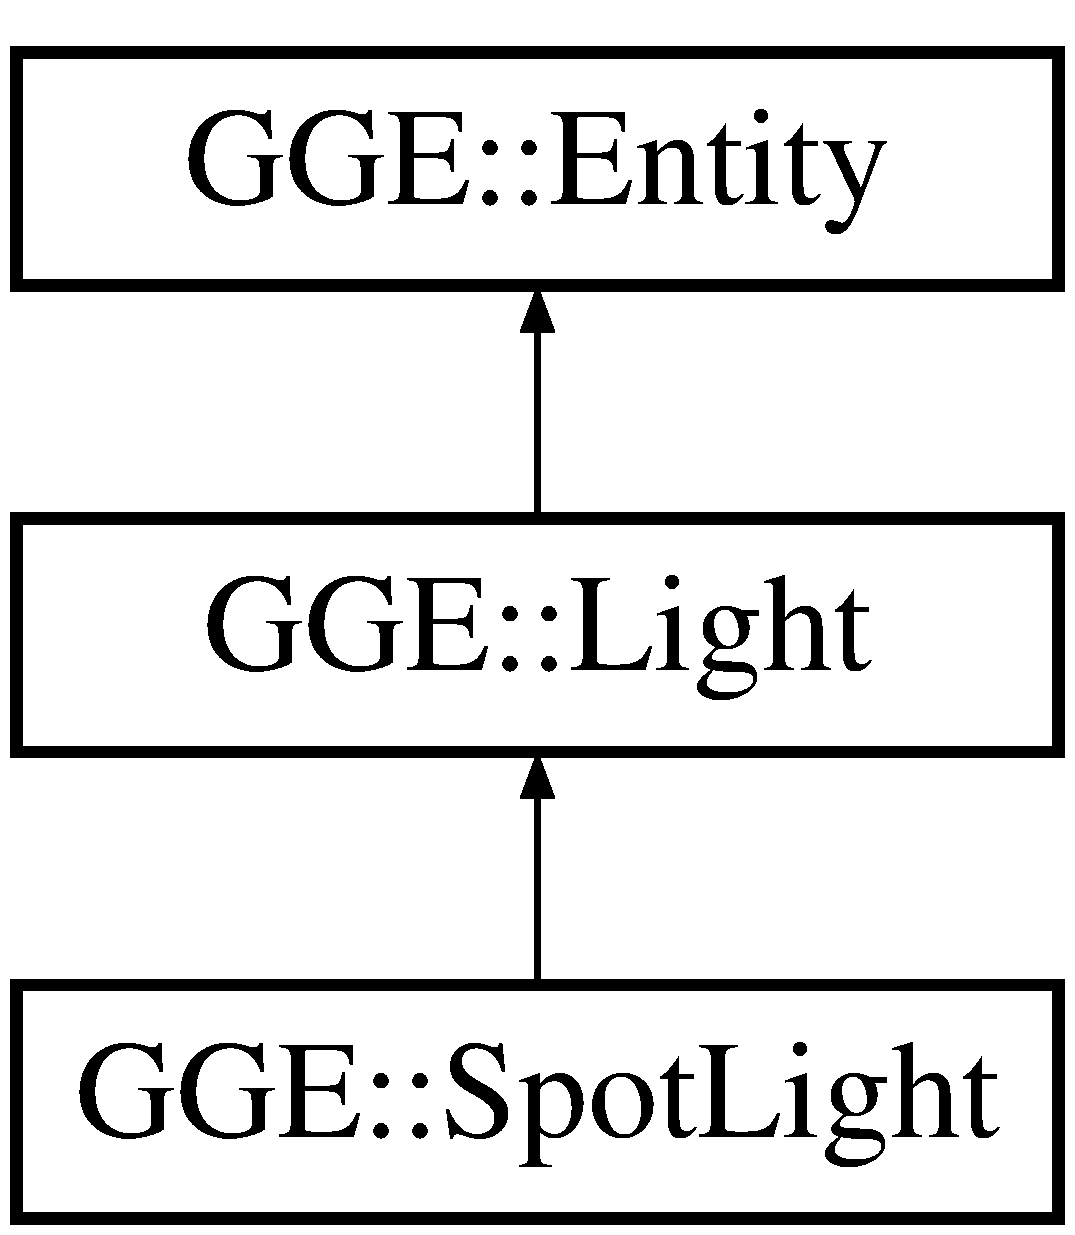
\includegraphics[height=3.000000cm]{class_g_g_e_1_1_spot_light}
\end{center}
\end{figure}
\subsection*{Public Member Functions}
\begin{DoxyCompactItemize}
\item 
\hyperlink{class_g_g_e_1_1_spot_light_a8cdfd89df0adae186c0a6e04adc03863}{Spot\+Light} (glm\+::vec3 \hyperlink{class_g_g_e_1_1_entity_a38a9fa01bfaf37ca415181ba6a179d3f}{position}, glm\+::vec3 \hyperlink{class_g_g_e_1_1_entity_a80c69365314541244f26e4a15b4223d8}{direction}, \hyperlink{namespace_g_g_e_aff43741fd756c83cbfd5d4d5cd9fcf41}{Color4} \hyperlink{class_g_g_e_1_1_light_a4d2f4605abc44637feac0d0312ce0717}{color})
\item 
\hyperlink{class_g_g_e_1_1_spot_light_ab08bdaac4b7a936c1af0401f9ba31295}{$\sim$\+Spot\+Light} ()
\end{DoxyCompactItemize}
\subsection*{Additional Inherited Members}


\subsection{Constructor \& Destructor Documentation}
\hypertarget{class_g_g_e_1_1_spot_light_a8cdfd89df0adae186c0a6e04adc03863}{\index{G\+G\+E\+::\+Spot\+Light@{G\+G\+E\+::\+Spot\+Light}!Spot\+Light@{Spot\+Light}}
\index{Spot\+Light@{Spot\+Light}!G\+G\+E\+::\+Spot\+Light@{G\+G\+E\+::\+Spot\+Light}}
\subsubsection[{Spot\+Light}]{\setlength{\rightskip}{0pt plus 5cm}G\+G\+E\+::\+Spot\+Light\+::\+Spot\+Light (
\begin{DoxyParamCaption}
\item[{glm\+::vec3}]{position, }
\item[{glm\+::vec3}]{direction, }
\item[{{\bf Color4}}]{color}
\end{DoxyParamCaption}
)}}\label{class_g_g_e_1_1_spot_light_a8cdfd89df0adae186c0a6e04adc03863}
\hypertarget{class_g_g_e_1_1_spot_light_ab08bdaac4b7a936c1af0401f9ba31295}{\index{G\+G\+E\+::\+Spot\+Light@{G\+G\+E\+::\+Spot\+Light}!````~Spot\+Light@{$\sim$\+Spot\+Light}}
\index{````~Spot\+Light@{$\sim$\+Spot\+Light}!G\+G\+E\+::\+Spot\+Light@{G\+G\+E\+::\+Spot\+Light}}
\subsubsection[{$\sim$\+Spot\+Light}]{\setlength{\rightskip}{0pt plus 5cm}G\+G\+E\+::\+Spot\+Light\+::$\sim$\+Spot\+Light (
\begin{DoxyParamCaption}
{}
\end{DoxyParamCaption}
)}}\label{class_g_g_e_1_1_spot_light_ab08bdaac4b7a936c1af0401f9ba31295}


The documentation for this class was generated from the following files\+:\begin{DoxyCompactItemize}
\item 
include/\hyperlink{light_8h}{light.\+h}\item 
src/\hyperlink{light_8cpp}{light.\+cpp}\end{DoxyCompactItemize}

\hypertarget{class_g_g_e_1_1_texture}{\section{G\+G\+E\+:\+:Texture Class Reference}
\label{class_g_g_e_1_1_texture}\index{G\+G\+E\+::\+Texture@{G\+G\+E\+::\+Texture}}
}


{\ttfamily \#include $<$texture.\+h$>$}

\subsection*{Public Member Functions}
\begin{DoxyCompactItemize}
\item 
\hyperlink{class_g_g_e_1_1_texture_af70bbf244600091e968aefc1ab27b73f}{Texture} (const unsigned int $\ast$image\+Data)
\item 
\hyperlink{class_g_g_e_1_1_texture_a3978c92ae0d7bec3aef3006d1cac802b}{Texture} (const char $\ast$filename, G\+Lenum \hyperlink{class_g_g_e_1_1_texture_a9fd9a4cf0a84fcd68b336c92d6d0514e}{texture\+Type})
\item 
\hyperlink{class_g_g_e_1_1_texture_a62700829f86e0b63e0cc4ee04202ee8d}{$\sim$\+Texture} ()
\item 
void \hyperlink{class_g_g_e_1_1_texture_a2c52e20a240d5ec5a9ba3c0d26454546}{bind} ()
\item 
G\+Luint \hyperlink{class_g_g_e_1_1_texture_a5e1ca37555586073c8014dde62c548f0}{get\+Texture\+I\+D} ()
\end{DoxyCompactItemize}
\subsection*{Static Public Attributes}
\begin{DoxyCompactItemize}
\item 
static \hyperlink{class_g_g_e_1_1_texture}{Texture} $\ast$ \hyperlink{class_g_g_e_1_1_texture_a0b90b74276704a2455ba2afa82cc13a7}{W\+H\+I\+T\+E}
\item 
static \hyperlink{class_g_g_e_1_1_texture}{Texture} $\ast$ \hyperlink{class_g_g_e_1_1_texture_a0ce25ba4515c038959da1d389d2c80da}{T\+R\+A\+N\+S\+P\+A\+R\+E\+N\+T}
\end{DoxyCompactItemize}
\subsection*{Private Member Functions}
\begin{DoxyCompactItemize}
\item 
void \hyperlink{class_g_g_e_1_1_texture_a0c017352f8273b7d55216b7ccccaa0ef}{init} ()
\end{DoxyCompactItemize}
\subsection*{Private Attributes}
\begin{DoxyCompactItemize}
\item 
G\+Luint \hyperlink{class_g_g_e_1_1_texture_a24eb48105f06bfe9c0b14d2ff84b50c6}{texture\+I\+D}
\item 
G\+Lenum \hyperlink{class_g_g_e_1_1_texture_a9fd9a4cf0a84fcd68b336c92d6d0514e}{texture\+Type}
\end{DoxyCompactItemize}
\subsection*{Static Private Attributes}
\begin{DoxyCompactItemize}
\item 
static G\+Luint \hyperlink{class_g_g_e_1_1_texture_ad1d7ae9c5c1c637d00d3002cf99e47e0}{current\+Texture} = 0
\end{DoxyCompactItemize}


\subsection{Constructor \& Destructor Documentation}
\hypertarget{class_g_g_e_1_1_texture_af70bbf244600091e968aefc1ab27b73f}{\index{G\+G\+E\+::\+Texture@{G\+G\+E\+::\+Texture}!Texture@{Texture}}
\index{Texture@{Texture}!G\+G\+E\+::\+Texture@{G\+G\+E\+::\+Texture}}
\subsubsection[{Texture}]{\setlength{\rightskip}{0pt plus 5cm}G\+G\+E\+::\+Texture\+::\+Texture (
\begin{DoxyParamCaption}
\item[{const unsigned int $\ast$}]{image\+Data}
\end{DoxyParamCaption}
)}}\label{class_g_g_e_1_1_texture_af70bbf244600091e968aefc1ab27b73f}
\hypertarget{class_g_g_e_1_1_texture_a3978c92ae0d7bec3aef3006d1cac802b}{\index{G\+G\+E\+::\+Texture@{G\+G\+E\+::\+Texture}!Texture@{Texture}}
\index{Texture@{Texture}!G\+G\+E\+::\+Texture@{G\+G\+E\+::\+Texture}}
\subsubsection[{Texture}]{\setlength{\rightskip}{0pt plus 5cm}G\+G\+E\+::\+Texture\+::\+Texture (
\begin{DoxyParamCaption}
\item[{const char $\ast$}]{filename, }
\item[{G\+Lenum}]{texture\+Type}
\end{DoxyParamCaption}
)}}\label{class_g_g_e_1_1_texture_a3978c92ae0d7bec3aef3006d1cac802b}
\hypertarget{class_g_g_e_1_1_texture_a62700829f86e0b63e0cc4ee04202ee8d}{\index{G\+G\+E\+::\+Texture@{G\+G\+E\+::\+Texture}!````~Texture@{$\sim$\+Texture}}
\index{````~Texture@{$\sim$\+Texture}!G\+G\+E\+::\+Texture@{G\+G\+E\+::\+Texture}}
\subsubsection[{$\sim$\+Texture}]{\setlength{\rightskip}{0pt plus 5cm}G\+G\+E\+::\+Texture\+::$\sim$\+Texture (
\begin{DoxyParamCaption}
{}
\end{DoxyParamCaption}
)}}\label{class_g_g_e_1_1_texture_a62700829f86e0b63e0cc4ee04202ee8d}


\subsection{Member Function Documentation}
\hypertarget{class_g_g_e_1_1_texture_a2c52e20a240d5ec5a9ba3c0d26454546}{\index{G\+G\+E\+::\+Texture@{G\+G\+E\+::\+Texture}!bind@{bind}}
\index{bind@{bind}!G\+G\+E\+::\+Texture@{G\+G\+E\+::\+Texture}}
\subsubsection[{bind}]{\setlength{\rightskip}{0pt plus 5cm}void G\+G\+E\+::\+Texture\+::bind (
\begin{DoxyParamCaption}
{}
\end{DoxyParamCaption}
)}}\label{class_g_g_e_1_1_texture_a2c52e20a240d5ec5a9ba3c0d26454546}
\hypertarget{class_g_g_e_1_1_texture_a5e1ca37555586073c8014dde62c548f0}{\index{G\+G\+E\+::\+Texture@{G\+G\+E\+::\+Texture}!get\+Texture\+I\+D@{get\+Texture\+I\+D}}
\index{get\+Texture\+I\+D@{get\+Texture\+I\+D}!G\+G\+E\+::\+Texture@{G\+G\+E\+::\+Texture}}
\subsubsection[{get\+Texture\+I\+D}]{\setlength{\rightskip}{0pt plus 5cm}G\+Luint G\+G\+E\+::\+Texture\+::get\+Texture\+I\+D (
\begin{DoxyParamCaption}
{}
\end{DoxyParamCaption}
)}}\label{class_g_g_e_1_1_texture_a5e1ca37555586073c8014dde62c548f0}
\hypertarget{class_g_g_e_1_1_texture_a0c017352f8273b7d55216b7ccccaa0ef}{\index{G\+G\+E\+::\+Texture@{G\+G\+E\+::\+Texture}!init@{init}}
\index{init@{init}!G\+G\+E\+::\+Texture@{G\+G\+E\+::\+Texture}}
\subsubsection[{init}]{\setlength{\rightskip}{0pt plus 5cm}void G\+G\+E\+::\+Texture\+::init (
\begin{DoxyParamCaption}
{}
\end{DoxyParamCaption}
)\hspace{0.3cm}{\ttfamily [private]}}}\label{class_g_g_e_1_1_texture_a0c017352f8273b7d55216b7ccccaa0ef}


\subsection{Member Data Documentation}
\hypertarget{class_g_g_e_1_1_texture_ad1d7ae9c5c1c637d00d3002cf99e47e0}{\index{G\+G\+E\+::\+Texture@{G\+G\+E\+::\+Texture}!current\+Texture@{current\+Texture}}
\index{current\+Texture@{current\+Texture}!G\+G\+E\+::\+Texture@{G\+G\+E\+::\+Texture}}
\subsubsection[{current\+Texture}]{\setlength{\rightskip}{0pt plus 5cm}G\+Luint G\+G\+E\+::\+Texture\+::current\+Texture = 0\hspace{0.3cm}{\ttfamily [static]}, {\ttfamily [private]}}}\label{class_g_g_e_1_1_texture_ad1d7ae9c5c1c637d00d3002cf99e47e0}
\hypertarget{class_g_g_e_1_1_texture_a24eb48105f06bfe9c0b14d2ff84b50c6}{\index{G\+G\+E\+::\+Texture@{G\+G\+E\+::\+Texture}!texture\+I\+D@{texture\+I\+D}}
\index{texture\+I\+D@{texture\+I\+D}!G\+G\+E\+::\+Texture@{G\+G\+E\+::\+Texture}}
\subsubsection[{texture\+I\+D}]{\setlength{\rightskip}{0pt plus 5cm}G\+Luint G\+G\+E\+::\+Texture\+::texture\+I\+D\hspace{0.3cm}{\ttfamily [private]}}}\label{class_g_g_e_1_1_texture_a24eb48105f06bfe9c0b14d2ff84b50c6}
\hypertarget{class_g_g_e_1_1_texture_a9fd9a4cf0a84fcd68b336c92d6d0514e}{\index{G\+G\+E\+::\+Texture@{G\+G\+E\+::\+Texture}!texture\+Type@{texture\+Type}}
\index{texture\+Type@{texture\+Type}!G\+G\+E\+::\+Texture@{G\+G\+E\+::\+Texture}}
\subsubsection[{texture\+Type}]{\setlength{\rightskip}{0pt plus 5cm}G\+Lenum G\+G\+E\+::\+Texture\+::texture\+Type\hspace{0.3cm}{\ttfamily [private]}}}\label{class_g_g_e_1_1_texture_a9fd9a4cf0a84fcd68b336c92d6d0514e}
\hypertarget{class_g_g_e_1_1_texture_a0ce25ba4515c038959da1d389d2c80da}{\index{G\+G\+E\+::\+Texture@{G\+G\+E\+::\+Texture}!T\+R\+A\+N\+S\+P\+A\+R\+E\+N\+T@{T\+R\+A\+N\+S\+P\+A\+R\+E\+N\+T}}
\index{T\+R\+A\+N\+S\+P\+A\+R\+E\+N\+T@{T\+R\+A\+N\+S\+P\+A\+R\+E\+N\+T}!G\+G\+E\+::\+Texture@{G\+G\+E\+::\+Texture}}
\subsubsection[{T\+R\+A\+N\+S\+P\+A\+R\+E\+N\+T}]{\setlength{\rightskip}{0pt plus 5cm}{\bf Texture}$\ast$ G\+G\+E\+::\+Texture\+::\+T\+R\+A\+N\+S\+P\+A\+R\+E\+N\+T\hspace{0.3cm}{\ttfamily [static]}}}\label{class_g_g_e_1_1_texture_a0ce25ba4515c038959da1d389d2c80da}
\hypertarget{class_g_g_e_1_1_texture_a0b90b74276704a2455ba2afa82cc13a7}{\index{G\+G\+E\+::\+Texture@{G\+G\+E\+::\+Texture}!W\+H\+I\+T\+E@{W\+H\+I\+T\+E}}
\index{W\+H\+I\+T\+E@{W\+H\+I\+T\+E}!G\+G\+E\+::\+Texture@{G\+G\+E\+::\+Texture}}
\subsubsection[{W\+H\+I\+T\+E}]{\setlength{\rightskip}{0pt plus 5cm}{\bf Texture}$\ast$ G\+G\+E\+::\+Texture\+::\+W\+H\+I\+T\+E\hspace{0.3cm}{\ttfamily [static]}}}\label{class_g_g_e_1_1_texture_a0b90b74276704a2455ba2afa82cc13a7}


The documentation for this class was generated from the following files\+:\begin{DoxyCompactItemize}
\item 
include/\hyperlink{texture_8h}{texture.\+h}\item 
src/\hyperlink{texture_8cpp}{texture.\+cpp}\end{DoxyCompactItemize}

\hypertarget{struct_g_g_e_1_1_texture_set}{\section{G\+G\+E\+:\+:Texture\+Set Struct Reference}
\label{struct_g_g_e_1_1_texture_set}\index{G\+G\+E\+::\+Texture\+Set@{G\+G\+E\+::\+Texture\+Set}}
}


{\ttfamily \#include $<$material.\+h$>$}

\subsection*{Public Member Functions}
\begin{DoxyCompactItemize}
\item 
\hyperlink{struct_g_g_e_1_1_texture_set_ad66546b1838684df6261193cb18f1deb}{Texture\+Set} ()
\end{DoxyCompactItemize}
\subsection*{Public Attributes}
\begin{DoxyCompactItemize}
\item 
\hyperlink{class_g_g_e_1_1_texture}{Texture} $\ast$ \hyperlink{struct_g_g_e_1_1_texture_set_a3f551a130debcd6a2339a395d8ecb955}{ambient\+Texture}
\item 
\hyperlink{class_g_g_e_1_1_texture}{Texture} $\ast$ \hyperlink{struct_g_g_e_1_1_texture_set_ac67540ccfc0af2dcb42ea873e144d198}{diffuse\+Texture}
\item 
\hyperlink{class_g_g_e_1_1_texture}{Texture} $\ast$ \hyperlink{struct_g_g_e_1_1_texture_set_a1e5cb782923be9a821b8515f850c5f4d}{specular\+Texture}
\item 
\hyperlink{class_g_g_e_1_1_texture}{Texture} $\ast$ \hyperlink{struct_g_g_e_1_1_texture_set_a1298833992b66a73ddaec01056f020ba}{normal\+Texture}
\end{DoxyCompactItemize}


\subsection{Constructor \& Destructor Documentation}
\hypertarget{struct_g_g_e_1_1_texture_set_ad66546b1838684df6261193cb18f1deb}{\index{G\+G\+E\+::\+Texture\+Set@{G\+G\+E\+::\+Texture\+Set}!Texture\+Set@{Texture\+Set}}
\index{Texture\+Set@{Texture\+Set}!G\+G\+E\+::\+Texture\+Set@{G\+G\+E\+::\+Texture\+Set}}
\subsubsection[{Texture\+Set}]{\setlength{\rightskip}{0pt plus 5cm}G\+G\+E\+::\+Texture\+Set\+::\+Texture\+Set (
\begin{DoxyParamCaption}
{}
\end{DoxyParamCaption}
)\hspace{0.3cm}{\ttfamily [inline]}}}\label{struct_g_g_e_1_1_texture_set_ad66546b1838684df6261193cb18f1deb}


\subsection{Member Data Documentation}
\hypertarget{struct_g_g_e_1_1_texture_set_a3f551a130debcd6a2339a395d8ecb955}{\index{G\+G\+E\+::\+Texture\+Set@{G\+G\+E\+::\+Texture\+Set}!ambient\+Texture@{ambient\+Texture}}
\index{ambient\+Texture@{ambient\+Texture}!G\+G\+E\+::\+Texture\+Set@{G\+G\+E\+::\+Texture\+Set}}
\subsubsection[{ambient\+Texture}]{\setlength{\rightskip}{0pt plus 5cm}{\bf Texture}$\ast$ G\+G\+E\+::\+Texture\+Set\+::ambient\+Texture}}\label{struct_g_g_e_1_1_texture_set_a3f551a130debcd6a2339a395d8ecb955}
\hypertarget{struct_g_g_e_1_1_texture_set_ac67540ccfc0af2dcb42ea873e144d198}{\index{G\+G\+E\+::\+Texture\+Set@{G\+G\+E\+::\+Texture\+Set}!diffuse\+Texture@{diffuse\+Texture}}
\index{diffuse\+Texture@{diffuse\+Texture}!G\+G\+E\+::\+Texture\+Set@{G\+G\+E\+::\+Texture\+Set}}
\subsubsection[{diffuse\+Texture}]{\setlength{\rightskip}{0pt plus 5cm}{\bf Texture} $\ast$ G\+G\+E\+::\+Texture\+Set\+::diffuse\+Texture}}\label{struct_g_g_e_1_1_texture_set_ac67540ccfc0af2dcb42ea873e144d198}
\hypertarget{struct_g_g_e_1_1_texture_set_a1298833992b66a73ddaec01056f020ba}{\index{G\+G\+E\+::\+Texture\+Set@{G\+G\+E\+::\+Texture\+Set}!normal\+Texture@{normal\+Texture}}
\index{normal\+Texture@{normal\+Texture}!G\+G\+E\+::\+Texture\+Set@{G\+G\+E\+::\+Texture\+Set}}
\subsubsection[{normal\+Texture}]{\setlength{\rightskip}{0pt plus 5cm}{\bf Texture} $\ast$ G\+G\+E\+::\+Texture\+Set\+::normal\+Texture}}\label{struct_g_g_e_1_1_texture_set_a1298833992b66a73ddaec01056f020ba}
\hypertarget{struct_g_g_e_1_1_texture_set_a1e5cb782923be9a821b8515f850c5f4d}{\index{G\+G\+E\+::\+Texture\+Set@{G\+G\+E\+::\+Texture\+Set}!specular\+Texture@{specular\+Texture}}
\index{specular\+Texture@{specular\+Texture}!G\+G\+E\+::\+Texture\+Set@{G\+G\+E\+::\+Texture\+Set}}
\subsubsection[{specular\+Texture}]{\setlength{\rightskip}{0pt plus 5cm}{\bf Texture} $\ast$ G\+G\+E\+::\+Texture\+Set\+::specular\+Texture}}\label{struct_g_g_e_1_1_texture_set_a1e5cb782923be9a821b8515f850c5f4d}


The documentation for this struct was generated from the following file\+:\begin{DoxyCompactItemize}
\item 
include/\hyperlink{material_8h}{material.\+h}\end{DoxyCompactItemize}

\hypertarget{class_g_g_e_1_1_window}{\section{G\+G\+E\+:\+:Window Class Reference}
\label{class_g_g_e_1_1_window}\index{G\+G\+E\+::\+Window@{G\+G\+E\+::\+Window}}
}


{\ttfamily \#include $<$window.\+h$>$}

\subsection*{Public Member Functions}
\begin{DoxyCompactItemize}
\item 
\hyperlink{class_g_g_e_1_1_window_a0be4c31554bea6a3e41b07b97ea4dd74}{Window} (int \hyperlink{class_g_g_e_1_1_window_a2aef17e23370755f4c3de24e527676ff}{height}, int \hyperlink{class_g_g_e_1_1_window_a5d878b7b885837f5062b516ecbdc22bf}{width}, bool \hyperlink{class_g_g_e_1_1_window_a43b2bb5a05e9f6d7af76086ce42145f2}{fullscreen}, char $\ast$\hyperlink{class_g_g_e_1_1_window_a9430276ac4c0ddc7e04be71772af4670}{title})
\item 
\hyperlink{class_g_g_e_1_1_window_aacf14cfd459d8c7cb78cb121327657c9}{$\sim$\+Window} ()
\item 
void \hyperlink{class_g_g_e_1_1_window_a705a031ad4ef0d5f6f08d715f2ec0e01}{set\+Render\+Function} (\hyperlink{namespace_g_g_e_ae2d6bfdcdfc2e210b6d827b4221a9dc4}{Render\+Function} \hyperlink{class_g_g_e_1_1_window_ac699c5d6c173adeea2f1e5cda44b8b9a}{render\+Function})
\item 
G\+L\+F\+Wwindow $\ast$ \hyperlink{class_g_g_e_1_1_window_a8ea51e37afd72bf174d51ea0b698a66c}{get\+G\+L\+F\+W\+Window} ()
\item 
int \hyperlink{class_g_g_e_1_1_window_ab69355bb29c63ba69fb75a8ac7b6a522}{get\+Height} ()
\item 
int \hyperlink{class_g_g_e_1_1_window_ad94d14a36c4ffcc4d97cedbe23828b7b}{get\+Width} ()
\item 
bool \hyperlink{class_g_g_e_1_1_window_af4ef9734314b74cb36417d8cabb6fb18}{is\+Fullscreen} ()
\item 
bool \hyperlink{class_g_g_e_1_1_window_ae2add48e60bfa9beb33b722176f9a0d5}{is\+Closed} ()
\item 
void \hyperlink{class_g_g_e_1_1_window_afd4c6a34bb54b77154e75fcb68fbee45}{close} ()
\item 
glm\+::mat4 \hyperlink{class_g_g_e_1_1_window_a0cb2e0dfb03bf3b9ffd0231d6e4e682c}{get\+Projection\+Matrix} ()
\item 
bool \hyperlink{class_g_g_e_1_1_window_a378a4b08b488eed0f30a4dfd552719f7}{render\+Frame} ()
\end{DoxyCompactItemize}
\subsection*{Private Member Functions}
\begin{DoxyCompactItemize}
\item 
void \hyperlink{class_g_g_e_1_1_window_aa7c54d7337b0e13e6c0c5d9ed26249f3}{init} ()
\end{DoxyCompactItemize}
\subsection*{Static Private Member Functions}
\begin{DoxyCompactItemize}
\item 
static void \hyperlink{class_g_g_e_1_1_window_a5eec12b16162d1b350173d75489abbf4}{resize\+Callback} (G\+L\+F\+Wwindow $\ast$\hyperlink{class_g_g_e_1_1_window_aefa5259b62d603d83ebf8963a019d73b}{window}, int new\+Width, int new\+Height)
\end{DoxyCompactItemize}
\subsection*{Private Attributes}
\begin{DoxyCompactItemize}
\item 
int \hyperlink{class_g_g_e_1_1_window_a2aef17e23370755f4c3de24e527676ff}{height}
\item 
int \hyperlink{class_g_g_e_1_1_window_a5d878b7b885837f5062b516ecbdc22bf}{width}
\item 
bool \hyperlink{class_g_g_e_1_1_window_a43b2bb5a05e9f6d7af76086ce42145f2}{fullscreen}
\item 
bool \hyperlink{class_g_g_e_1_1_window_a0cba23a6e1296e5f1d539e87b177d678}{should\+Close}
\item 
char $\ast$ \hyperlink{class_g_g_e_1_1_window_a9430276ac4c0ddc7e04be71772af4670}{title}
\item 
G\+L\+F\+Wwindow $\ast$ \hyperlink{class_g_g_e_1_1_window_aefa5259b62d603d83ebf8963a019d73b}{window}
\item 
double \hyperlink{class_g_g_e_1_1_window_a4cea6995dfa84431c5169dd3208fbda8}{time\+Since\+Last\+Frame}
\item 
double \hyperlink{class_g_g_e_1_1_window_ab93d7f77e803a854ef5188d5ce039838}{last\+Frame\+Time}
\item 
glm\+::mat4 \hyperlink{class_g_g_e_1_1_window_acc1dfe541ecdf8c1ca08eec451ea7aba}{projection\+Matrix}
\item 
\hyperlink{namespace_g_g_e_ae2d6bfdcdfc2e210b6d827b4221a9dc4}{Render\+Function} \hyperlink{class_g_g_e_1_1_window_ac699c5d6c173adeea2f1e5cda44b8b9a}{render\+Function}
\end{DoxyCompactItemize}
\subsection*{Static Private Attributes}
\begin{DoxyCompactItemize}
\item 
static std\+::list$<$ \hyperlink{class_g_g_e_1_1_window}{Window} $\ast$ $>$ \hyperlink{class_g_g_e_1_1_window_a2ab7c16795aa37b881760cff6b487f06}{windows}
\end{DoxyCompactItemize}


\subsection{Constructor \& Destructor Documentation}
\hypertarget{class_g_g_e_1_1_window_a0be4c31554bea6a3e41b07b97ea4dd74}{\index{G\+G\+E\+::\+Window@{G\+G\+E\+::\+Window}!Window@{Window}}
\index{Window@{Window}!G\+G\+E\+::\+Window@{G\+G\+E\+::\+Window}}
\subsubsection[{Window}]{\setlength{\rightskip}{0pt plus 5cm}G\+G\+E\+::\+Window\+::\+Window (
\begin{DoxyParamCaption}
\item[{int}]{height, }
\item[{int}]{width, }
\item[{bool}]{fullscreen, }
\item[{char $\ast$}]{title}
\end{DoxyParamCaption}
)}}\label{class_g_g_e_1_1_window_a0be4c31554bea6a3e41b07b97ea4dd74}
\hypertarget{class_g_g_e_1_1_window_aacf14cfd459d8c7cb78cb121327657c9}{\index{G\+G\+E\+::\+Window@{G\+G\+E\+::\+Window}!````~Window@{$\sim$\+Window}}
\index{````~Window@{$\sim$\+Window}!G\+G\+E\+::\+Window@{G\+G\+E\+::\+Window}}
\subsubsection[{$\sim$\+Window}]{\setlength{\rightskip}{0pt plus 5cm}G\+G\+E\+::\+Window\+::$\sim$\+Window (
\begin{DoxyParamCaption}
{}
\end{DoxyParamCaption}
)}}\label{class_g_g_e_1_1_window_aacf14cfd459d8c7cb78cb121327657c9}


\subsection{Member Function Documentation}
\hypertarget{class_g_g_e_1_1_window_afd4c6a34bb54b77154e75fcb68fbee45}{\index{G\+G\+E\+::\+Window@{G\+G\+E\+::\+Window}!close@{close}}
\index{close@{close}!G\+G\+E\+::\+Window@{G\+G\+E\+::\+Window}}
\subsubsection[{close}]{\setlength{\rightskip}{0pt plus 5cm}void G\+G\+E\+::\+Window\+::close (
\begin{DoxyParamCaption}
{}
\end{DoxyParamCaption}
)}}\label{class_g_g_e_1_1_window_afd4c6a34bb54b77154e75fcb68fbee45}
\hypertarget{class_g_g_e_1_1_window_a8ea51e37afd72bf174d51ea0b698a66c}{\index{G\+G\+E\+::\+Window@{G\+G\+E\+::\+Window}!get\+G\+L\+F\+W\+Window@{get\+G\+L\+F\+W\+Window}}
\index{get\+G\+L\+F\+W\+Window@{get\+G\+L\+F\+W\+Window}!G\+G\+E\+::\+Window@{G\+G\+E\+::\+Window}}
\subsubsection[{get\+G\+L\+F\+W\+Window}]{\setlength{\rightskip}{0pt plus 5cm}G\+L\+F\+Wwindow $\ast$ G\+G\+E\+::\+Window\+::get\+G\+L\+F\+W\+Window (
\begin{DoxyParamCaption}
{}
\end{DoxyParamCaption}
)}}\label{class_g_g_e_1_1_window_a8ea51e37afd72bf174d51ea0b698a66c}
\hypertarget{class_g_g_e_1_1_window_ab69355bb29c63ba69fb75a8ac7b6a522}{\index{G\+G\+E\+::\+Window@{G\+G\+E\+::\+Window}!get\+Height@{get\+Height}}
\index{get\+Height@{get\+Height}!G\+G\+E\+::\+Window@{G\+G\+E\+::\+Window}}
\subsubsection[{get\+Height}]{\setlength{\rightskip}{0pt plus 5cm}int G\+G\+E\+::\+Window\+::get\+Height (
\begin{DoxyParamCaption}
{}
\end{DoxyParamCaption}
)}}\label{class_g_g_e_1_1_window_ab69355bb29c63ba69fb75a8ac7b6a522}
\hypertarget{class_g_g_e_1_1_window_a0cb2e0dfb03bf3b9ffd0231d6e4e682c}{\index{G\+G\+E\+::\+Window@{G\+G\+E\+::\+Window}!get\+Projection\+Matrix@{get\+Projection\+Matrix}}
\index{get\+Projection\+Matrix@{get\+Projection\+Matrix}!G\+G\+E\+::\+Window@{G\+G\+E\+::\+Window}}
\subsubsection[{get\+Projection\+Matrix}]{\setlength{\rightskip}{0pt plus 5cm}glm\+::mat4 G\+G\+E\+::\+Window\+::get\+Projection\+Matrix (
\begin{DoxyParamCaption}
{}
\end{DoxyParamCaption}
)}}\label{class_g_g_e_1_1_window_a0cb2e0dfb03bf3b9ffd0231d6e4e682c}
\hypertarget{class_g_g_e_1_1_window_ad94d14a36c4ffcc4d97cedbe23828b7b}{\index{G\+G\+E\+::\+Window@{G\+G\+E\+::\+Window}!get\+Width@{get\+Width}}
\index{get\+Width@{get\+Width}!G\+G\+E\+::\+Window@{G\+G\+E\+::\+Window}}
\subsubsection[{get\+Width}]{\setlength{\rightskip}{0pt plus 5cm}int G\+G\+E\+::\+Window\+::get\+Width (
\begin{DoxyParamCaption}
{}
\end{DoxyParamCaption}
)}}\label{class_g_g_e_1_1_window_ad94d14a36c4ffcc4d97cedbe23828b7b}
\hypertarget{class_g_g_e_1_1_window_aa7c54d7337b0e13e6c0c5d9ed26249f3}{\index{G\+G\+E\+::\+Window@{G\+G\+E\+::\+Window}!init@{init}}
\index{init@{init}!G\+G\+E\+::\+Window@{G\+G\+E\+::\+Window}}
\subsubsection[{init}]{\setlength{\rightskip}{0pt plus 5cm}void G\+G\+E\+::\+Window\+::init (
\begin{DoxyParamCaption}
{}
\end{DoxyParamCaption}
)\hspace{0.3cm}{\ttfamily [private]}}}\label{class_g_g_e_1_1_window_aa7c54d7337b0e13e6c0c5d9ed26249f3}
\hypertarget{class_g_g_e_1_1_window_ae2add48e60bfa9beb33b722176f9a0d5}{\index{G\+G\+E\+::\+Window@{G\+G\+E\+::\+Window}!is\+Closed@{is\+Closed}}
\index{is\+Closed@{is\+Closed}!G\+G\+E\+::\+Window@{G\+G\+E\+::\+Window}}
\subsubsection[{is\+Closed}]{\setlength{\rightskip}{0pt plus 5cm}bool G\+G\+E\+::\+Window\+::is\+Closed (
\begin{DoxyParamCaption}
{}
\end{DoxyParamCaption}
)}}\label{class_g_g_e_1_1_window_ae2add48e60bfa9beb33b722176f9a0d5}
\hypertarget{class_g_g_e_1_1_window_af4ef9734314b74cb36417d8cabb6fb18}{\index{G\+G\+E\+::\+Window@{G\+G\+E\+::\+Window}!is\+Fullscreen@{is\+Fullscreen}}
\index{is\+Fullscreen@{is\+Fullscreen}!G\+G\+E\+::\+Window@{G\+G\+E\+::\+Window}}
\subsubsection[{is\+Fullscreen}]{\setlength{\rightskip}{0pt plus 5cm}bool G\+G\+E\+::\+Window\+::is\+Fullscreen (
\begin{DoxyParamCaption}
{}
\end{DoxyParamCaption}
)}}\label{class_g_g_e_1_1_window_af4ef9734314b74cb36417d8cabb6fb18}
\hypertarget{class_g_g_e_1_1_window_a378a4b08b488eed0f30a4dfd552719f7}{\index{G\+G\+E\+::\+Window@{G\+G\+E\+::\+Window}!render\+Frame@{render\+Frame}}
\index{render\+Frame@{render\+Frame}!G\+G\+E\+::\+Window@{G\+G\+E\+::\+Window}}
\subsubsection[{render\+Frame}]{\setlength{\rightskip}{0pt plus 5cm}bool G\+G\+E\+::\+Window\+::render\+Frame (
\begin{DoxyParamCaption}
{}
\end{DoxyParamCaption}
)}}\label{class_g_g_e_1_1_window_a378a4b08b488eed0f30a4dfd552719f7}
\hypertarget{class_g_g_e_1_1_window_a5eec12b16162d1b350173d75489abbf4}{\index{G\+G\+E\+::\+Window@{G\+G\+E\+::\+Window}!resize\+Callback@{resize\+Callback}}
\index{resize\+Callback@{resize\+Callback}!G\+G\+E\+::\+Window@{G\+G\+E\+::\+Window}}
\subsubsection[{resize\+Callback}]{\setlength{\rightskip}{0pt plus 5cm}void G\+G\+E\+::\+Window\+::resize\+Callback (
\begin{DoxyParamCaption}
\item[{G\+L\+F\+Wwindow $\ast$}]{window, }
\item[{int}]{new\+Width, }
\item[{int}]{new\+Height}
\end{DoxyParamCaption}
)\hspace{0.3cm}{\ttfamily [static]}, {\ttfamily [private]}}}\label{class_g_g_e_1_1_window_a5eec12b16162d1b350173d75489abbf4}
\hypertarget{class_g_g_e_1_1_window_a705a031ad4ef0d5f6f08d715f2ec0e01}{\index{G\+G\+E\+::\+Window@{G\+G\+E\+::\+Window}!set\+Render\+Function@{set\+Render\+Function}}
\index{set\+Render\+Function@{set\+Render\+Function}!G\+G\+E\+::\+Window@{G\+G\+E\+::\+Window}}
\subsubsection[{set\+Render\+Function}]{\setlength{\rightskip}{0pt plus 5cm}void G\+G\+E\+::\+Window\+::set\+Render\+Function (
\begin{DoxyParamCaption}
\item[{{\bf Render\+Function}}]{render\+Function}
\end{DoxyParamCaption}
)}}\label{class_g_g_e_1_1_window_a705a031ad4ef0d5f6f08d715f2ec0e01}


\subsection{Member Data Documentation}
\hypertarget{class_g_g_e_1_1_window_a43b2bb5a05e9f6d7af76086ce42145f2}{\index{G\+G\+E\+::\+Window@{G\+G\+E\+::\+Window}!fullscreen@{fullscreen}}
\index{fullscreen@{fullscreen}!G\+G\+E\+::\+Window@{G\+G\+E\+::\+Window}}
\subsubsection[{fullscreen}]{\setlength{\rightskip}{0pt plus 5cm}bool G\+G\+E\+::\+Window\+::fullscreen\hspace{0.3cm}{\ttfamily [private]}}}\label{class_g_g_e_1_1_window_a43b2bb5a05e9f6d7af76086ce42145f2}
\hypertarget{class_g_g_e_1_1_window_a2aef17e23370755f4c3de24e527676ff}{\index{G\+G\+E\+::\+Window@{G\+G\+E\+::\+Window}!height@{height}}
\index{height@{height}!G\+G\+E\+::\+Window@{G\+G\+E\+::\+Window}}
\subsubsection[{height}]{\setlength{\rightskip}{0pt plus 5cm}int G\+G\+E\+::\+Window\+::height\hspace{0.3cm}{\ttfamily [private]}}}\label{class_g_g_e_1_1_window_a2aef17e23370755f4c3de24e527676ff}
\hypertarget{class_g_g_e_1_1_window_ab93d7f77e803a854ef5188d5ce039838}{\index{G\+G\+E\+::\+Window@{G\+G\+E\+::\+Window}!last\+Frame\+Time@{last\+Frame\+Time}}
\index{last\+Frame\+Time@{last\+Frame\+Time}!G\+G\+E\+::\+Window@{G\+G\+E\+::\+Window}}
\subsubsection[{last\+Frame\+Time}]{\setlength{\rightskip}{0pt plus 5cm}double G\+G\+E\+::\+Window\+::last\+Frame\+Time\hspace{0.3cm}{\ttfamily [private]}}}\label{class_g_g_e_1_1_window_ab93d7f77e803a854ef5188d5ce039838}
\hypertarget{class_g_g_e_1_1_window_acc1dfe541ecdf8c1ca08eec451ea7aba}{\index{G\+G\+E\+::\+Window@{G\+G\+E\+::\+Window}!projection\+Matrix@{projection\+Matrix}}
\index{projection\+Matrix@{projection\+Matrix}!G\+G\+E\+::\+Window@{G\+G\+E\+::\+Window}}
\subsubsection[{projection\+Matrix}]{\setlength{\rightskip}{0pt plus 5cm}glm\+::mat4 G\+G\+E\+::\+Window\+::projection\+Matrix\hspace{0.3cm}{\ttfamily [private]}}}\label{class_g_g_e_1_1_window_acc1dfe541ecdf8c1ca08eec451ea7aba}
\hypertarget{class_g_g_e_1_1_window_ac699c5d6c173adeea2f1e5cda44b8b9a}{\index{G\+G\+E\+::\+Window@{G\+G\+E\+::\+Window}!render\+Function@{render\+Function}}
\index{render\+Function@{render\+Function}!G\+G\+E\+::\+Window@{G\+G\+E\+::\+Window}}
\subsubsection[{render\+Function}]{\setlength{\rightskip}{0pt plus 5cm}{\bf Render\+Function} G\+G\+E\+::\+Window\+::render\+Function\hspace{0.3cm}{\ttfamily [private]}}}\label{class_g_g_e_1_1_window_ac699c5d6c173adeea2f1e5cda44b8b9a}
\hypertarget{class_g_g_e_1_1_window_a0cba23a6e1296e5f1d539e87b177d678}{\index{G\+G\+E\+::\+Window@{G\+G\+E\+::\+Window}!should\+Close@{should\+Close}}
\index{should\+Close@{should\+Close}!G\+G\+E\+::\+Window@{G\+G\+E\+::\+Window}}
\subsubsection[{should\+Close}]{\setlength{\rightskip}{0pt plus 5cm}bool G\+G\+E\+::\+Window\+::should\+Close\hspace{0.3cm}{\ttfamily [private]}}}\label{class_g_g_e_1_1_window_a0cba23a6e1296e5f1d539e87b177d678}
\hypertarget{class_g_g_e_1_1_window_a4cea6995dfa84431c5169dd3208fbda8}{\index{G\+G\+E\+::\+Window@{G\+G\+E\+::\+Window}!time\+Since\+Last\+Frame@{time\+Since\+Last\+Frame}}
\index{time\+Since\+Last\+Frame@{time\+Since\+Last\+Frame}!G\+G\+E\+::\+Window@{G\+G\+E\+::\+Window}}
\subsubsection[{time\+Since\+Last\+Frame}]{\setlength{\rightskip}{0pt plus 5cm}double G\+G\+E\+::\+Window\+::time\+Since\+Last\+Frame\hspace{0.3cm}{\ttfamily [private]}}}\label{class_g_g_e_1_1_window_a4cea6995dfa84431c5169dd3208fbda8}
\hypertarget{class_g_g_e_1_1_window_a9430276ac4c0ddc7e04be71772af4670}{\index{G\+G\+E\+::\+Window@{G\+G\+E\+::\+Window}!title@{title}}
\index{title@{title}!G\+G\+E\+::\+Window@{G\+G\+E\+::\+Window}}
\subsubsection[{title}]{\setlength{\rightskip}{0pt plus 5cm}char$\ast$ G\+G\+E\+::\+Window\+::title\hspace{0.3cm}{\ttfamily [private]}}}\label{class_g_g_e_1_1_window_a9430276ac4c0ddc7e04be71772af4670}
\hypertarget{class_g_g_e_1_1_window_a5d878b7b885837f5062b516ecbdc22bf}{\index{G\+G\+E\+::\+Window@{G\+G\+E\+::\+Window}!width@{width}}
\index{width@{width}!G\+G\+E\+::\+Window@{G\+G\+E\+::\+Window}}
\subsubsection[{width}]{\setlength{\rightskip}{0pt plus 5cm}int G\+G\+E\+::\+Window\+::width\hspace{0.3cm}{\ttfamily [private]}}}\label{class_g_g_e_1_1_window_a5d878b7b885837f5062b516ecbdc22bf}
\hypertarget{class_g_g_e_1_1_window_aefa5259b62d603d83ebf8963a019d73b}{\index{G\+G\+E\+::\+Window@{G\+G\+E\+::\+Window}!window@{window}}
\index{window@{window}!G\+G\+E\+::\+Window@{G\+G\+E\+::\+Window}}
\subsubsection[{window}]{\setlength{\rightskip}{0pt plus 5cm}G\+L\+F\+Wwindow$\ast$ G\+G\+E\+::\+Window\+::window\hspace{0.3cm}{\ttfamily [private]}}}\label{class_g_g_e_1_1_window_aefa5259b62d603d83ebf8963a019d73b}
\hypertarget{class_g_g_e_1_1_window_a2ab7c16795aa37b881760cff6b487f06}{\index{G\+G\+E\+::\+Window@{G\+G\+E\+::\+Window}!windows@{windows}}
\index{windows@{windows}!G\+G\+E\+::\+Window@{G\+G\+E\+::\+Window}}
\subsubsection[{windows}]{\setlength{\rightskip}{0pt plus 5cm}std\+::list$<$ {\bf Window} $\ast$ $>$ G\+G\+E\+::\+Window\+::windows\hspace{0.3cm}{\ttfamily [static]}, {\ttfamily [private]}}}\label{class_g_g_e_1_1_window_a2ab7c16795aa37b881760cff6b487f06}


The documentation for this class was generated from the following files\+:\begin{DoxyCompactItemize}
\item 
include/\hyperlink{window_8h}{window.\+h}\item 
src/\hyperlink{window_8cpp}{window.\+cpp}\end{DoxyCompactItemize}

\chapter{File Documentation}
\hypertarget{application_8h}{\section{include/application.h File Reference}
\label{application_8h}\index{include/application.\+h@{include/application.\+h}}
}
{\ttfamily \#include \char`\"{}glew.\+h\char`\"{}}\\*
{\ttfamily \#include \char`\"{}glfw3.\+h\char`\"{}}\\*
{\ttfamily \#include \char`\"{}window.\+h\char`\"{}}\\*
\subsection*{Classes}
\begin{DoxyCompactItemize}
\item 
class \hyperlink{class_g_g_e_1_1_application}{G\+G\+E\+::\+Application}
\end{DoxyCompactItemize}
\subsection*{Namespaces}
\begin{DoxyCompactItemize}
\item 
 \hyperlink{namespace_g_g_e}{G\+G\+E}
\end{DoxyCompactItemize}

\hypertarget{camera_8h}{\section{include/camera.h File Reference}
\label{camera_8h}\index{include/camera.\+h@{include/camera.\+h}}
}
{\ttfamily \#include $<$list$>$}\\*
{\ttfamily \#include \char`\"{}entity.\+h\char`\"{}}\\*
{\ttfamily \#include \char`\"{}glm.\+hpp\char`\"{}}\\*
{\ttfamily \#include \char`\"{}geometry.\+h\char`\"{}}\\*
\subsection*{Classes}
\begin{DoxyCompactItemize}
\item 
class \hyperlink{class_g_g_e_1_1_camera}{G\+G\+E\+::\+Camera}
\end{DoxyCompactItemize}
\subsection*{Namespaces}
\begin{DoxyCompactItemize}
\item 
 \hyperlink{namespace_g_g_e}{G\+G\+E}
\end{DoxyCompactItemize}

\hypertarget{color_8h}{\section{include/color.h File Reference}
\label{color_8h}\index{include/color.\+h@{include/color.\+h}}
}
{\ttfamily \#include \char`\"{}glm.\+hpp\char`\"{}}\\*
\subsection*{Namespaces}
\begin{DoxyCompactItemize}
\item 
 \hyperlink{namespace_g_g_e}{G\+G\+E}
\item 
 \hyperlink{namespace_g_g_e_1_1_color}{G\+G\+E\+::\+Color}
\end{DoxyCompactItemize}
\subsection*{Typedefs}
\begin{DoxyCompactItemize}
\item 
typedef glm\+::vec4 \hyperlink{namespace_g_g_e_aff43741fd756c83cbfd5d4d5cd9fcf41}{G\+G\+E\+::\+Color4}
\item 
typedef glm\+::vec3 \hyperlink{namespace_g_g_e_ae2829723f010eeffbb96282f99792546}{G\+G\+E\+::\+Color3}
\end{DoxyCompactItemize}
\subsection*{Variables}
\begin{DoxyCompactItemize}
\item 
static const Color4 \hyperlink{namespace_g_g_e_1_1_color_a98e8bfcace99241c67bc5d1921c459da}{G\+G\+E\+::\+Color\+::\+R\+E\+D} = Color4(1.\+0f, 0.\+0f, 0.\+0f, 1.\+0f)
\item 
static const Color4 \hyperlink{namespace_g_g_e_1_1_color_a8d6c7c4aee508c3a1181009632277eb3}{G\+G\+E\+::\+Color\+::\+B\+L\+U\+E} = Color4(0.\+0f, 1.\+0f, 0.\+0f, 1.\+0f)
\item 
static const Color4 \hyperlink{namespace_g_g_e_1_1_color_a26095ccaba67ad0c12df2b8731fa2c1a}{G\+G\+E\+::\+Color\+::\+G\+R\+E\+E\+N} = Color4(0.\+0f, 0.\+0f, 1.\+0f, 1.\+0f)
\item 
static const Color4 \hyperlink{namespace_g_g_e_1_1_color_a431b29401359e9cb0ecade51b388b2c8}{G\+G\+E\+::\+Color\+::\+W\+H\+I\+T\+E} = Color4(1.\+0f, 1.\+0f, 1.\+0f, 1.\+0f)
\item 
static const Color4 \hyperlink{namespace_g_g_e_1_1_color_a88f2db25cc7bf1d38ee7fa3d87f01294}{G\+G\+E\+::\+Color\+::\+B\+L\+A\+C\+K} = Color4(0.\+0f, 0.\+0f, 0.\+0f, 1.\+0f)
\item 
static const Color4 \hyperlink{namespace_g_g_e_1_1_color_aca92af9d049df379ee0b8eb327fe27f6}{G\+G\+E\+::\+Color\+::\+N\+O\+N\+E} = Color4(0.\+0f, 0.\+0f, 0.\+0f, 0.\+0f)
\item 
static const Color4 \hyperlink{namespace_g_g_e_1_1_color_a20973cadec5f187b10c2789739cd6833}{G\+G\+E\+::\+Color\+::\+T\+R\+A\+N\+S\+P\+A\+R\+E\+N\+T} = N\+O\+N\+E
\end{DoxyCompactItemize}

\hypertarget{entity_8h}{\section{include/entity.h File Reference}
\label{entity_8h}\index{include/entity.\+h@{include/entity.\+h}}
}
{\ttfamily \#include \char`\"{}glm.\+hpp\char`\"{}}\\*
{\ttfamily \#include \char`\"{}gtc/quaternion.\+hpp\char`\"{}}\\*
\subsection*{Classes}
\begin{DoxyCompactItemize}
\item 
class \hyperlink{class_g_g_e_1_1_entity}{G\+G\+E\+::\+Entity}
\end{DoxyCompactItemize}
\subsection*{Namespaces}
\begin{DoxyCompactItemize}
\item 
 \hyperlink{namespace_g_g_e}{G\+G\+E}
\end{DoxyCompactItemize}

\hypertarget{geometry_8h}{\section{include/geometry.h File Reference}
\label{geometry_8h}\index{include/geometry.\+h@{include/geometry.\+h}}
}
{\ttfamily \#include \char`\"{}glm.\+hpp\char`\"{}}\\*
\subsection*{Namespaces}
\begin{DoxyCompactItemize}
\item 
 \hyperlink{namespace_g_g_e}{G\+G\+E}
\end{DoxyCompactItemize}
\subsection*{Macros}
\begin{DoxyCompactItemize}
\item 
\#define \hyperlink{geometry_8h_a053a42d378b8fbf4da2fbf6a451389a8}{X\+\_\+\+U\+N\+I\+T\+\_\+\+V\+E\+C\+T\+O\+R}~glm\+::vec3(1.\+0, 0.\+0, 0.\+0)
\item 
\#define \hyperlink{geometry_8h_a9c03fcc53f25d6a9c2dfd8fc229686e4}{N\+E\+G\+A\+T\+I\+V\+E\+\_\+\+X\+\_\+\+U\+N\+I\+T\+\_\+\+V\+E\+C\+T\+O\+R}~glm\+::vec3(-\/1.\+0, 0.\+0, 0.\+0)
\item 
\#define \hyperlink{geometry_8h_a7d6711c6186da4b0a5340c87437ecea1}{Y\+\_\+\+U\+N\+I\+T\+\_\+\+V\+E\+C\+T\+O\+R}~glm\+::vec3(0.\+0, 1.\+0, 0.\+0)
\item 
\#define \hyperlink{geometry_8h_aefa9b70f35188b4d44b758bb20af3e43}{N\+E\+G\+A\+T\+I\+V\+E\+\_\+\+Y\+\_\+\+U\+N\+I\+T\+\_\+\+V\+E\+C\+T\+O\+R}~glm\+::vec3(0.\+0, -\/1.\+0, 0.\+0)
\item 
\#define \hyperlink{geometry_8h_a83eddec4e136e15a7623359ab8392c5f}{Z\+\_\+\+U\+N\+I\+T\+\_\+\+V\+E\+C\+T\+O\+R}~glm\+::vec3(0.\+0, 0.\+0, 1.\+0)
\item 
\#define \hyperlink{geometry_8h_a7c1e97999a0f6c6009169d9a94c7ce33}{N\+E\+G\+A\+T\+I\+V\+E\+\_\+\+Z\+\_\+\+U\+N\+I\+T\+\_\+\+V\+E\+C\+T\+O\+R}~glm\+::vec3(0.\+0, 0.\+0, -\/1.\+0)
\item 
\#define \hyperlink{geometry_8h_a598a3330b3c21701223ee0ca14316eca}{P\+I}~3.\+14159
\item 
\#define \hyperlink{geometry_8h_a643d7a22f1a1e10b41c8b195d62c2d35}{D\+E\+G\+R\+E\+E\+S\+\_\+\+T\+O\+\_\+\+R\+A\+D\+I\+A\+N\+S}(x)~((x) $\ast$ \hyperlink{geometry_8h_a598a3330b3c21701223ee0ca14316eca}{P\+I} / 180.\+0)
\item 
\#define \hyperlink{geometry_8h_aa52892493f91f06ffbaf93dcbcd5b3d3}{R\+A\+D\+I\+A\+N\+S\+\_\+\+T\+O\+\_\+\+D\+E\+G\+R\+E\+E\+S}(x)~((x) $\ast$ 180.\+0 / \hyperlink{geometry_8h_a598a3330b3c21701223ee0ca14316eca}{P\+I})
\end{DoxyCompactItemize}


\subsection{Macro Definition Documentation}
\hypertarget{geometry_8h_a643d7a22f1a1e10b41c8b195d62c2d35}{\index{geometry.\+h@{geometry.\+h}!D\+E\+G\+R\+E\+E\+S\+\_\+\+T\+O\+\_\+\+R\+A\+D\+I\+A\+N\+S@{D\+E\+G\+R\+E\+E\+S\+\_\+\+T\+O\+\_\+\+R\+A\+D\+I\+A\+N\+S}}
\index{D\+E\+G\+R\+E\+E\+S\+\_\+\+T\+O\+\_\+\+R\+A\+D\+I\+A\+N\+S@{D\+E\+G\+R\+E\+E\+S\+\_\+\+T\+O\+\_\+\+R\+A\+D\+I\+A\+N\+S}!geometry.\+h@{geometry.\+h}}
\subsubsection[{D\+E\+G\+R\+E\+E\+S\+\_\+\+T\+O\+\_\+\+R\+A\+D\+I\+A\+N\+S}]{\setlength{\rightskip}{0pt plus 5cm}\#define D\+E\+G\+R\+E\+E\+S\+\_\+\+T\+O\+\_\+\+R\+A\+D\+I\+A\+N\+S(
\begin{DoxyParamCaption}
\item[{}]{x}
\end{DoxyParamCaption}
)~((x) $\ast$ {\bf P\+I} / 180.\+0)}}\label{geometry_8h_a643d7a22f1a1e10b41c8b195d62c2d35}
\hypertarget{geometry_8h_a9c03fcc53f25d6a9c2dfd8fc229686e4}{\index{geometry.\+h@{geometry.\+h}!N\+E\+G\+A\+T\+I\+V\+E\+\_\+\+X\+\_\+\+U\+N\+I\+T\+\_\+\+V\+E\+C\+T\+O\+R@{N\+E\+G\+A\+T\+I\+V\+E\+\_\+\+X\+\_\+\+U\+N\+I\+T\+\_\+\+V\+E\+C\+T\+O\+R}}
\index{N\+E\+G\+A\+T\+I\+V\+E\+\_\+\+X\+\_\+\+U\+N\+I\+T\+\_\+\+V\+E\+C\+T\+O\+R@{N\+E\+G\+A\+T\+I\+V\+E\+\_\+\+X\+\_\+\+U\+N\+I\+T\+\_\+\+V\+E\+C\+T\+O\+R}!geometry.\+h@{geometry.\+h}}
\subsubsection[{N\+E\+G\+A\+T\+I\+V\+E\+\_\+\+X\+\_\+\+U\+N\+I\+T\+\_\+\+V\+E\+C\+T\+O\+R}]{\setlength{\rightskip}{0pt plus 5cm}\#define N\+E\+G\+A\+T\+I\+V\+E\+\_\+\+X\+\_\+\+U\+N\+I\+T\+\_\+\+V\+E\+C\+T\+O\+R~glm\+::vec3(-\/1.\+0, 0.\+0, 0.\+0)}}\label{geometry_8h_a9c03fcc53f25d6a9c2dfd8fc229686e4}
\hypertarget{geometry_8h_aefa9b70f35188b4d44b758bb20af3e43}{\index{geometry.\+h@{geometry.\+h}!N\+E\+G\+A\+T\+I\+V\+E\+\_\+\+Y\+\_\+\+U\+N\+I\+T\+\_\+\+V\+E\+C\+T\+O\+R@{N\+E\+G\+A\+T\+I\+V\+E\+\_\+\+Y\+\_\+\+U\+N\+I\+T\+\_\+\+V\+E\+C\+T\+O\+R}}
\index{N\+E\+G\+A\+T\+I\+V\+E\+\_\+\+Y\+\_\+\+U\+N\+I\+T\+\_\+\+V\+E\+C\+T\+O\+R@{N\+E\+G\+A\+T\+I\+V\+E\+\_\+\+Y\+\_\+\+U\+N\+I\+T\+\_\+\+V\+E\+C\+T\+O\+R}!geometry.\+h@{geometry.\+h}}
\subsubsection[{N\+E\+G\+A\+T\+I\+V\+E\+\_\+\+Y\+\_\+\+U\+N\+I\+T\+\_\+\+V\+E\+C\+T\+O\+R}]{\setlength{\rightskip}{0pt plus 5cm}\#define N\+E\+G\+A\+T\+I\+V\+E\+\_\+\+Y\+\_\+\+U\+N\+I\+T\+\_\+\+V\+E\+C\+T\+O\+R~glm\+::vec3(0.\+0, -\/1.\+0, 0.\+0)}}\label{geometry_8h_aefa9b70f35188b4d44b758bb20af3e43}
\hypertarget{geometry_8h_a7c1e97999a0f6c6009169d9a94c7ce33}{\index{geometry.\+h@{geometry.\+h}!N\+E\+G\+A\+T\+I\+V\+E\+\_\+\+Z\+\_\+\+U\+N\+I\+T\+\_\+\+V\+E\+C\+T\+O\+R@{N\+E\+G\+A\+T\+I\+V\+E\+\_\+\+Z\+\_\+\+U\+N\+I\+T\+\_\+\+V\+E\+C\+T\+O\+R}}
\index{N\+E\+G\+A\+T\+I\+V\+E\+\_\+\+Z\+\_\+\+U\+N\+I\+T\+\_\+\+V\+E\+C\+T\+O\+R@{N\+E\+G\+A\+T\+I\+V\+E\+\_\+\+Z\+\_\+\+U\+N\+I\+T\+\_\+\+V\+E\+C\+T\+O\+R}!geometry.\+h@{geometry.\+h}}
\subsubsection[{N\+E\+G\+A\+T\+I\+V\+E\+\_\+\+Z\+\_\+\+U\+N\+I\+T\+\_\+\+V\+E\+C\+T\+O\+R}]{\setlength{\rightskip}{0pt plus 5cm}\#define N\+E\+G\+A\+T\+I\+V\+E\+\_\+\+Z\+\_\+\+U\+N\+I\+T\+\_\+\+V\+E\+C\+T\+O\+R~glm\+::vec3(0.\+0, 0.\+0, -\/1.\+0)}}\label{geometry_8h_a7c1e97999a0f6c6009169d9a94c7ce33}
\hypertarget{geometry_8h_a598a3330b3c21701223ee0ca14316eca}{\index{geometry.\+h@{geometry.\+h}!P\+I@{P\+I}}
\index{P\+I@{P\+I}!geometry.\+h@{geometry.\+h}}
\subsubsection[{P\+I}]{\setlength{\rightskip}{0pt plus 5cm}\#define P\+I~3.\+14159}}\label{geometry_8h_a598a3330b3c21701223ee0ca14316eca}
\hypertarget{geometry_8h_aa52892493f91f06ffbaf93dcbcd5b3d3}{\index{geometry.\+h@{geometry.\+h}!R\+A\+D\+I\+A\+N\+S\+\_\+\+T\+O\+\_\+\+D\+E\+G\+R\+E\+E\+S@{R\+A\+D\+I\+A\+N\+S\+\_\+\+T\+O\+\_\+\+D\+E\+G\+R\+E\+E\+S}}
\index{R\+A\+D\+I\+A\+N\+S\+\_\+\+T\+O\+\_\+\+D\+E\+G\+R\+E\+E\+S@{R\+A\+D\+I\+A\+N\+S\+\_\+\+T\+O\+\_\+\+D\+E\+G\+R\+E\+E\+S}!geometry.\+h@{geometry.\+h}}
\subsubsection[{R\+A\+D\+I\+A\+N\+S\+\_\+\+T\+O\+\_\+\+D\+E\+G\+R\+E\+E\+S}]{\setlength{\rightskip}{0pt plus 5cm}\#define R\+A\+D\+I\+A\+N\+S\+\_\+\+T\+O\+\_\+\+D\+E\+G\+R\+E\+E\+S(
\begin{DoxyParamCaption}
\item[{}]{x}
\end{DoxyParamCaption}
)~((x) $\ast$ 180.\+0 / {\bf P\+I})}}\label{geometry_8h_aa52892493f91f06ffbaf93dcbcd5b3d3}
\hypertarget{geometry_8h_a053a42d378b8fbf4da2fbf6a451389a8}{\index{geometry.\+h@{geometry.\+h}!X\+\_\+\+U\+N\+I\+T\+\_\+\+V\+E\+C\+T\+O\+R@{X\+\_\+\+U\+N\+I\+T\+\_\+\+V\+E\+C\+T\+O\+R}}
\index{X\+\_\+\+U\+N\+I\+T\+\_\+\+V\+E\+C\+T\+O\+R@{X\+\_\+\+U\+N\+I\+T\+\_\+\+V\+E\+C\+T\+O\+R}!geometry.\+h@{geometry.\+h}}
\subsubsection[{X\+\_\+\+U\+N\+I\+T\+\_\+\+V\+E\+C\+T\+O\+R}]{\setlength{\rightskip}{0pt plus 5cm}\#define X\+\_\+\+U\+N\+I\+T\+\_\+\+V\+E\+C\+T\+O\+R~glm\+::vec3(1.\+0, 0.\+0, 0.\+0)}}\label{geometry_8h_a053a42d378b8fbf4da2fbf6a451389a8}
\hypertarget{geometry_8h_a7d6711c6186da4b0a5340c87437ecea1}{\index{geometry.\+h@{geometry.\+h}!Y\+\_\+\+U\+N\+I\+T\+\_\+\+V\+E\+C\+T\+O\+R@{Y\+\_\+\+U\+N\+I\+T\+\_\+\+V\+E\+C\+T\+O\+R}}
\index{Y\+\_\+\+U\+N\+I\+T\+\_\+\+V\+E\+C\+T\+O\+R@{Y\+\_\+\+U\+N\+I\+T\+\_\+\+V\+E\+C\+T\+O\+R}!geometry.\+h@{geometry.\+h}}
\subsubsection[{Y\+\_\+\+U\+N\+I\+T\+\_\+\+V\+E\+C\+T\+O\+R}]{\setlength{\rightskip}{0pt plus 5cm}\#define Y\+\_\+\+U\+N\+I\+T\+\_\+\+V\+E\+C\+T\+O\+R~glm\+::vec3(0.\+0, 1.\+0, 0.\+0)}}\label{geometry_8h_a7d6711c6186da4b0a5340c87437ecea1}
\hypertarget{geometry_8h_a83eddec4e136e15a7623359ab8392c5f}{\index{geometry.\+h@{geometry.\+h}!Z\+\_\+\+U\+N\+I\+T\+\_\+\+V\+E\+C\+T\+O\+R@{Z\+\_\+\+U\+N\+I\+T\+\_\+\+V\+E\+C\+T\+O\+R}}
\index{Z\+\_\+\+U\+N\+I\+T\+\_\+\+V\+E\+C\+T\+O\+R@{Z\+\_\+\+U\+N\+I\+T\+\_\+\+V\+E\+C\+T\+O\+R}!geometry.\+h@{geometry.\+h}}
\subsubsection[{Z\+\_\+\+U\+N\+I\+T\+\_\+\+V\+E\+C\+T\+O\+R}]{\setlength{\rightskip}{0pt plus 5cm}\#define Z\+\_\+\+U\+N\+I\+T\+\_\+\+V\+E\+C\+T\+O\+R~glm\+::vec3(0.\+0, 0.\+0, 1.\+0)}}\label{geometry_8h_a83eddec4e136e15a7623359ab8392c5f}

\hypertarget{light_8h}{\section{include/light.h File Reference}
\label{light_8h}\index{include/light.\+h@{include/light.\+h}}
}
{\ttfamily \#include \char`\"{}glm.\+hpp\char`\"{}}\\*
{\ttfamily \#include \char`\"{}entity.\+h\char`\"{}}\\*
{\ttfamily \#include \char`\"{}color.\+h\char`\"{}}\\*
\subsection*{Classes}
\begin{DoxyCompactItemize}
\item 
class \hyperlink{class_g_g_e_1_1_light}{G\+G\+E\+::\+Light}
\item 
class \hyperlink{class_g_g_e_1_1_point_light}{G\+G\+E\+::\+Point\+Light}
\item 
class \hyperlink{class_g_g_e_1_1_ambient_light}{G\+G\+E\+::\+Ambient\+Light}
\item 
class \hyperlink{class_g_g_e_1_1_spot_light}{G\+G\+E\+::\+Spot\+Light}
\end{DoxyCompactItemize}
\subsection*{Namespaces}
\begin{DoxyCompactItemize}
\item 
 \hyperlink{namespace_g_g_e}{G\+G\+E}
\end{DoxyCompactItemize}
\subsection*{Enumerations}
\begin{DoxyCompactItemize}
\item 
enum \hyperlink{namespace_g_g_e_abf6b28d5fd20f356a5ad88fec0789eff}{G\+G\+E\+::\+Light\+Type} \{ \hyperlink{namespace_g_g_e_abf6b28d5fd20f356a5ad88fec0789effa10682e47f2dadd21bc173c5563132707}{G\+G\+E\+::\+L\+I\+G\+H\+T\+\_\+\+P\+O\+I\+N\+T}, 
\hyperlink{namespace_g_g_e_abf6b28d5fd20f356a5ad88fec0789effa6e91747b8f895b2df6e810582d808cf2}{G\+G\+E\+::\+L\+I\+G\+H\+T\+\_\+\+A\+M\+B\+I\+E\+N\+T}, 
\hyperlink{namespace_g_g_e_abf6b28d5fd20f356a5ad88fec0789effa6a6aca641e9a8de1341e8c9826e28c3e}{G\+G\+E\+::\+L\+I\+G\+H\+T\+\_\+\+S\+P\+O\+T}
 \}
\end{DoxyCompactItemize}

\hypertarget{material_8h}{\section{include/material.h File Reference}
\label{material_8h}\index{include/material.\+h@{include/material.\+h}}
}
{\ttfamily \#include $<$vector$>$}\\*
{\ttfamily \#include \char`\"{}glew.\+h\char`\"{}}\\*
{\ttfamily \#include \char`\"{}glfw3.\+h\char`\"{}}\\*
{\ttfamily \#include \char`\"{}texture.\+h\char`\"{}}\\*
{\ttfamily \#include \char`\"{}color.\+h\char`\"{}}\\*
\subsection*{Classes}
\begin{DoxyCompactItemize}
\item 
struct \hyperlink{struct_g_g_e_1_1_lighting_properties}{G\+G\+E\+::\+Lighting\+Properties}
\item 
struct \hyperlink{struct_g_g_e_1_1_texture_set}{G\+G\+E\+::\+Texture\+Set}
\item 
class \hyperlink{class_g_g_e_1_1_material}{G\+G\+E\+::\+Material}
\end{DoxyCompactItemize}
\subsection*{Namespaces}
\begin{DoxyCompactItemize}
\item 
 \hyperlink{namespace_g_g_e}{G\+G\+E}
\end{DoxyCompactItemize}
\subsection*{Typedefs}
\begin{DoxyCompactItemize}
\item 
typedef struct \\*
\hyperlink{struct_g_g_e_1_1_lighting_properties}{G\+G\+E\+::\+Lighting\+Properties} \hyperlink{namespace_g_g_e_a3cb8bb0b982d877997c93103c48e2592}{G\+G\+E\+::\+Lighting\+Properties}
\item 
typedef struct \hyperlink{struct_g_g_e_1_1_texture_set}{G\+G\+E\+::\+Texture\+Set} \hyperlink{namespace_g_g_e_ac7a8b0e1f9b7fdd11002ac1259a61278}{G\+G\+E\+::\+Texture\+Set}
\end{DoxyCompactItemize}
\subsection*{Enumerations}
\begin{DoxyCompactItemize}
\item 
enum \hyperlink{namespace_g_g_e_ad1102da762de1f99e787ff6a9453ef73}{G\+G\+E\+::\+Lighting\+Colors} \{ \\*
\hyperlink{namespace_g_g_e_ad1102da762de1f99e787ff6a9453ef73a0e2b52fdda401f9c5e7adcf88e551051}{G\+G\+E\+::\+A\+M\+B\+I\+E\+N\+T\+\_\+\+C\+O\+L\+O\+R}, 
\hyperlink{namespace_g_g_e_ad1102da762de1f99e787ff6a9453ef73a1adb8b6b5f332801c5123c8085fdf330}{G\+G\+E\+::\+D\+I\+F\+F\+U\+S\+E\+\_\+\+C\+O\+L\+O\+R}, 
\hyperlink{namespace_g_g_e_ad1102da762de1f99e787ff6a9453ef73a988671a427177535c02bb476971bc99e}{G\+G\+E\+::\+S\+P\+E\+C\+U\+L\+A\+R\+\_\+\+C\+O\+L\+O\+R}, 
\hyperlink{namespace_g_g_e_ad1102da762de1f99e787ff6a9453ef73a5abf49a870da850605260bd1c8c75f78}{G\+G\+E\+::\+T\+R\+A\+N\+S\+M\+I\+S\+S\+I\+O\+N\+\_\+\+C\+O\+L\+O\+R}, 
\\*
\hyperlink{namespace_g_g_e_ad1102da762de1f99e787ff6a9453ef73ab4b3d5a51b4207d7e0a70d169ff31913}{G\+G\+E\+::\+E\+M\+I\+T\+T\+A\+N\+C\+E\+\_\+\+C\+O\+L\+O\+R}
 \}
\item 
enum \hyperlink{namespace_g_g_e_aa6c57ddad718cba85e6cbd1437b81405}{G\+G\+E\+::\+Light\+Travel\+Properties} \{ \hyperlink{namespace_g_g_e_aa6c57ddad718cba85e6cbd1437b81405aab01896fe3a7559065fa6a6d1a4300cd}{G\+G\+E\+::\+S\+H\+I\+N\+I\+N\+E\+S\+S}, 
\hyperlink{namespace_g_g_e_aa6c57ddad718cba85e6cbd1437b81405a26a173b3290d0b73d8284247b340772a}{G\+G\+E\+::\+I\+N\+D\+E\+X\+\_\+\+O\+F\+\_\+\+R\+E\+F\+R\+A\+C\+T\+I\+O\+N}, 
\hyperlink{namespace_g_g_e_aa6c57ddad718cba85e6cbd1437b81405a0da0949a9e51b4fc3d41b4cea9f8d246}{G\+G\+E\+::\+D\+I\+S\+S\+O\+L\+V\+E}
 \}
\end{DoxyCompactItemize}

\hypertarget{mesh_8h}{\section{include/mesh.h File Reference}
\label{mesh_8h}\index{include/mesh.\+h@{include/mesh.\+h}}
}
{\ttfamily \#include $<$vector$>$}\\*
{\ttfamily \#include \char`\"{}glew.\+h\char`\"{}}\\*
{\ttfamily \#include \char`\"{}glfw3.\+h\char`\"{}}\\*
{\ttfamily \#include \char`\"{}glm.\+hpp\char`\"{}}\\*
{\ttfamily \#include \char`\"{}texture.\+h\char`\"{}}\\*
{\ttfamily \#include \char`\"{}program.\+h\char`\"{}}\\*
{\ttfamily \#include \char`\"{}entity.\+h\char`\"{}}\\*
{\ttfamily \#include \char`\"{}shape.\+h\char`\"{}}\\*
\subsection*{Classes}
\begin{DoxyCompactItemize}
\item 
class \hyperlink{class_g_g_e_1_1_mesh}{G\+G\+E\+::\+Mesh}
\end{DoxyCompactItemize}
\subsection*{Namespaces}
\begin{DoxyCompactItemize}
\item 
 \hyperlink{namespace_g_g_e}{G\+G\+E}
\end{DoxyCompactItemize}

\hypertarget{program_8h}{\section{include/program.h File Reference}
\label{program_8h}\index{include/program.\+h@{include/program.\+h}}
}
{\ttfamily \#include $<$vector$>$}\\*
{\ttfamily \#include $<$list$>$}\\*
{\ttfamily \#include \char`\"{}shader.\+h\char`\"{}}\\*
{\ttfamily \#include \char`\"{}glew.\+h\char`\"{}}\\*
{\ttfamily \#include \char`\"{}glfw3.\+h\char`\"{}}\\*
{\ttfamily \#include \char`\"{}glm.\+hpp\char`\"{}}\\*
\subsection*{Classes}
\begin{DoxyCompactItemize}
\item 
class \hyperlink{class_g_g_e_1_1_program}{G\+G\+E\+::\+Program}
\end{DoxyCompactItemize}
\subsection*{Namespaces}
\begin{DoxyCompactItemize}
\item 
 \hyperlink{namespace_g_g_e}{G\+G\+E}
\end{DoxyCompactItemize}

\hypertarget{shader_8h}{\section{include/shader.h File Reference}
\label{shader_8h}\index{include/shader.\+h@{include/shader.\+h}}
}
{\ttfamily \#include $<$string$>$}\\*
{\ttfamily \#include \char`\"{}glew.\+h\char`\"{}}\\*
{\ttfamily \#include \char`\"{}glfw3.\+h\char`\"{}}\\*
\subsection*{Classes}
\begin{DoxyCompactItemize}
\item 
class \hyperlink{class_g_g_e_1_1_shader}{G\+G\+E\+::\+Shader}
\end{DoxyCompactItemize}
\subsection*{Namespaces}
\begin{DoxyCompactItemize}
\item 
 \hyperlink{namespace_g_g_e}{G\+G\+E}
\end{DoxyCompactItemize}

\hypertarget{shape_8h}{\section{include/shape.h File Reference}
\label{shape_8h}\index{include/shape.\+h@{include/shape.\+h}}
}
{\ttfamily \#include $<$vector$>$}\\*
{\ttfamily \#include \char`\"{}glew.\+h\char`\"{}}\\*
{\ttfamily \#include \char`\"{}glfw3.\+h\char`\"{}}\\*
{\ttfamily \#include \char`\"{}material.\+h\char`\"{}}\\*
\subsection*{Classes}
\begin{DoxyCompactItemize}
\item 
struct \hyperlink{struct_g_g_e_1_1_coordinate_set}{G\+G\+E\+::\+Coordinate\+Set}
\item 
class \hyperlink{class_g_g_e_1_1_shape}{G\+G\+E\+::\+Shape}
\end{DoxyCompactItemize}
\subsection*{Namespaces}
\begin{DoxyCompactItemize}
\item 
 \hyperlink{namespace_g_g_e}{G\+G\+E}
\end{DoxyCompactItemize}
\subsection*{Typedefs}
\begin{DoxyCompactItemize}
\item 
typedef struct \hyperlink{struct_g_g_e_1_1_coordinate_set}{G\+G\+E\+::\+Coordinate\+Set} \hyperlink{namespace_g_g_e_a7e11417ae8ffddb46f0338f25ebf2051}{G\+G\+E\+::\+Coordinate\+Set}
\end{DoxyCompactItemize}

\hypertarget{texture_8h}{\section{include/texture.h File Reference}
\label{texture_8h}\index{include/texture.\+h@{include/texture.\+h}}
}
{\ttfamily \#include $<$glew.\+h$>$}\\*
{\ttfamily \#include $<$glfw3.\+h$>$}\\*
\subsection*{Classes}
\begin{DoxyCompactItemize}
\item 
class \hyperlink{class_g_g_e_1_1_texture}{G\+G\+E\+::\+Texture}
\end{DoxyCompactItemize}
\subsection*{Namespaces}
\begin{DoxyCompactItemize}
\item 
 \hyperlink{namespace_g_g_e}{G\+G\+E}
\end{DoxyCompactItemize}

\hypertarget{window_8h}{\section{include/window.h File Reference}
\label{window_8h}\index{include/window.\+h@{include/window.\+h}}
}
{\ttfamily \#include $<$list$>$}\\*
{\ttfamily \#include \char`\"{}glew.\+h\char`\"{}}\\*
{\ttfamily \#include \char`\"{}glfw3.\+h\char`\"{}}\\*
{\ttfamily \#include \char`\"{}glm.\+hpp\char`\"{}}\\*
\subsection*{Classes}
\begin{DoxyCompactItemize}
\item 
class \hyperlink{class_g_g_e_1_1_window}{G\+G\+E\+::\+Window}
\end{DoxyCompactItemize}
\subsection*{Namespaces}
\begin{DoxyCompactItemize}
\item 
 \hyperlink{namespace_g_g_e}{G\+G\+E}
\end{DoxyCompactItemize}
\subsection*{Typedefs}
\begin{DoxyCompactItemize}
\item 
typedef void($\ast$ \hyperlink{namespace_g_g_e_ae2d6bfdcdfc2e210b6d827b4221a9dc4}{G\+G\+E\+::\+Render\+Function} )(double time\+Since\+Last\+Frame)
\end{DoxyCompactItemize}

\hypertarget{application_8cpp}{\section{src/application.cpp File Reference}
\label{application_8cpp}\index{src/application.\+cpp@{src/application.\+cpp}}
}
{\ttfamily \#include $<$stdio.\+h$>$}\\*
{\ttfamily \#include \char`\"{}application.\+h\char`\"{}}\\*
\subsection*{Namespaces}
\begin{DoxyCompactItemize}
\item 
 \hyperlink{namespace_g_g_e}{G\+G\+E}
\end{DoxyCompactItemize}

\hypertarget{camera_8cpp}{\section{src/camera.cpp File Reference}
\label{camera_8cpp}\index{src/camera.\+cpp@{src/camera.\+cpp}}
}
{\ttfamily \#include $<$geometry.\+h$>$}\\*
{\ttfamily \#include \char`\"{}gtc/matrix\+\_\+transform.\+hpp\char`\"{}}\\*
{\ttfamily \#include \char`\"{}gtc/type\+\_\+ptr.\+hpp\char`\"{}}\\*
{\ttfamily \#include \char`\"{}gtx/rotate\+\_\+vector.\+hpp\char`\"{}}\\*
{\ttfamily \#include \char`\"{}program.\+h\char`\"{}}\\*
{\ttfamily \#include \char`\"{}camera.\+h\char`\"{}}\\*
\subsection*{Namespaces}
\begin{DoxyCompactItemize}
\item 
 \hyperlink{namespace_g_g_e}{G\+G\+E}
\end{DoxyCompactItemize}

\hypertarget{entity_8cpp}{\section{src/entity.cpp File Reference}
\label{entity_8cpp}\index{src/entity.\+cpp@{src/entity.\+cpp}}
}
{\ttfamily \#include \char`\"{}entity.\+h\char`\"{}}\\*
{\ttfamily \#include \char`\"{}gtx/rotate\+\_\+vector.\+hpp\char`\"{}}\\*
\subsection*{Namespaces}
\begin{DoxyCompactItemize}
\item 
 \hyperlink{namespace_g_g_e}{G\+G\+E}
\end{DoxyCompactItemize}

\hypertarget{light_8cpp}{\section{src/light.cpp File Reference}
\label{light_8cpp}\index{src/light.\+cpp@{src/light.\+cpp}}
}
{\ttfamily \#include \char`\"{}light.\+h\char`\"{}}\\*
\subsection*{Namespaces}
\begin{DoxyCompactItemize}
\item 
 \hyperlink{namespace_g_g_e}{G\+G\+E}
\end{DoxyCompactItemize}

\hypertarget{main_8cpp}{\section{src/main.cpp File Reference}
\label{main_8cpp}\index{src/main.\+cpp@{src/main.\+cpp}}
}
{\ttfamily \#include $<$vector$>$}\\*
{\ttfamily \#include $<$stdio.\+h$>$}\\*
{\ttfamily \#include $<$camera.\+h$>$}\\*
{\ttfamily \#include \char`\"{}application.\+h\char`\"{}}\\*
{\ttfamily \#include \char`\"{}shader.\+h\char`\"{}}\\*
{\ttfamily \#include \char`\"{}mesh.\+h\char`\"{}}\\*
{\ttfamily \#include \char`\"{}texture.\+h\char`\"{}}\\*
{\ttfamily \#include \char`\"{}program.\+h\char`\"{}}\\*
{\ttfamily \#include \char`\"{}geometry.\+h\char`\"{}}\\*
\subsection*{Functions}
\begin{DoxyCompactItemize}
\item 
void \hyperlink{main_8cpp_aa8282e07b3588f21a8b10caac984f3ec}{setup\+Scene} ()
\item 
void \hyperlink{main_8cpp_a0b9e239c8889734711f29fe45551605b}{key\+Callback} (G\+L\+F\+Wwindow $\ast$window, int key, int scancode, int action, int mods)
\item 
void \hyperlink{main_8cpp_a86a4350073f51aaa6d7ffe99483de0fe}{handle\+Input} ()
\item 
void \hyperlink{main_8cpp_a30dbe68e652430b2bd7f76a35ff1532d}{cursor\+Move\+Callback} (G\+L\+F\+Wwindow $\ast$window, double xpos, double ypos)
\item 
void \hyperlink{main_8cpp_a14142d114a12aad9433697c2d3851f06}{render\+Function} (double time\+Since\+Last\+Frame)
\item 
int \hyperlink{main_8cpp_a3c04138a5bfe5d72780bb7e82a18e627}{main} (int argc, char $\ast$$\ast$argv)
\end{DoxyCompactItemize}
\subsection*{Variables}
\begin{DoxyCompactItemize}
\item 
\hyperlink{class_g_g_e_1_1_application}{Application} $\ast$ \hyperlink{main_8cpp_a08c031f46c2bc800cdd9286852d26504}{app}
\item 
\hyperlink{class_g_g_e_1_1_program}{Program} $\ast$ \hyperlink{main_8cpp_abbc44d602bd51853e0165bbb21d6f5cc}{p}
\item 
\hyperlink{class_g_g_e_1_1_program}{Program} $\ast$ \hyperlink{main_8cpp_a96317c9b772fe6e84ce735692905c3e1}{tex\+P}
\item 
\hyperlink{class_g_g_e_1_1_texture}{Texture} $\ast$ \hyperlink{main_8cpp_aa9a93f0c8415e5c11c6112ff98a1574b}{brick\+Tex}
\item 
\hyperlink{class_g_g_e_1_1_mesh}{Mesh} $\ast$ \hyperlink{main_8cpp_ab47b77b0f7916a070a0c49e5ec3ac423}{t1}
\item 
\hyperlink{class_g_g_e_1_1_mesh}{Mesh} $\ast$ \hyperlink{main_8cpp_ae98054e39d0b88ddbeb15a63cf1ee2a0}{t2}
\item 
\hyperlink{class_g_g_e_1_1_mesh}{Mesh} $\ast$ \hyperlink{main_8cpp_a2f808901531bf6692c890c86206c3c81}{t3}
\item 
\hyperlink{class_g_g_e_1_1_mesh}{Mesh} $\ast$ \hyperlink{main_8cpp_a918c9fcf384a4cce91d12bd8ccb83c25}{square}
\item 
\hyperlink{class_g_g_e_1_1_mesh}{Mesh} $\ast$ \hyperlink{main_8cpp_a46dcd1bba82ee2dbc8dd56647eca9219}{textured\+Triangle}
\item 
\hyperlink{class_g_g_e_1_1_mesh}{Mesh} $\ast$ \hyperlink{main_8cpp_a52f7498f4a875c8186aeb19e235043ac}{obj\+Cube}
\item 
\hyperlink{class_g_g_e_1_1_camera}{Camera} $\ast$ \hyperlink{main_8cpp_a82f7081245eb70cf78c0a189cfab9e19}{cam}
\item 
G\+Lenum \hyperlink{main_8cpp_a9027aa147a2ef3f7ad71f86d229add1f}{polygon\+Mode} = G\+L\+\_\+\+F\+I\+L\+L
\end{DoxyCompactItemize}


\subsection{Function Documentation}
\hypertarget{main_8cpp_a30dbe68e652430b2bd7f76a35ff1532d}{\index{main.\+cpp@{main.\+cpp}!cursor\+Move\+Callback@{cursor\+Move\+Callback}}
\index{cursor\+Move\+Callback@{cursor\+Move\+Callback}!main.\+cpp@{main.\+cpp}}
\subsubsection[{cursor\+Move\+Callback}]{\setlength{\rightskip}{0pt plus 5cm}void cursor\+Move\+Callback (
\begin{DoxyParamCaption}
\item[{G\+L\+F\+Wwindow $\ast$}]{window, }
\item[{double}]{xpos, }
\item[{double}]{ypos}
\end{DoxyParamCaption}
)}}\label{main_8cpp_a30dbe68e652430b2bd7f76a35ff1532d}
\hypertarget{main_8cpp_a86a4350073f51aaa6d7ffe99483de0fe}{\index{main.\+cpp@{main.\+cpp}!handle\+Input@{handle\+Input}}
\index{handle\+Input@{handle\+Input}!main.\+cpp@{main.\+cpp}}
\subsubsection[{handle\+Input}]{\setlength{\rightskip}{0pt plus 5cm}void handle\+Input (
\begin{DoxyParamCaption}
{}
\end{DoxyParamCaption}
)}}\label{main_8cpp_a86a4350073f51aaa6d7ffe99483de0fe}
\hypertarget{main_8cpp_a0b9e239c8889734711f29fe45551605b}{\index{main.\+cpp@{main.\+cpp}!key\+Callback@{key\+Callback}}
\index{key\+Callback@{key\+Callback}!main.\+cpp@{main.\+cpp}}
\subsubsection[{key\+Callback}]{\setlength{\rightskip}{0pt plus 5cm}void key\+Callback (
\begin{DoxyParamCaption}
\item[{G\+L\+F\+Wwindow $\ast$}]{window, }
\item[{int}]{key, }
\item[{int}]{scancode, }
\item[{int}]{action, }
\item[{int}]{mods}
\end{DoxyParamCaption}
)}}\label{main_8cpp_a0b9e239c8889734711f29fe45551605b}
\hypertarget{main_8cpp_a3c04138a5bfe5d72780bb7e82a18e627}{\index{main.\+cpp@{main.\+cpp}!main@{main}}
\index{main@{main}!main.\+cpp@{main.\+cpp}}
\subsubsection[{main}]{\setlength{\rightskip}{0pt plus 5cm}int main (
\begin{DoxyParamCaption}
\item[{int}]{argc, }
\item[{char $\ast$$\ast$}]{argv}
\end{DoxyParamCaption}
)}}\label{main_8cpp_a3c04138a5bfe5d72780bb7e82a18e627}
\hypertarget{main_8cpp_a14142d114a12aad9433697c2d3851f06}{\index{main.\+cpp@{main.\+cpp}!render\+Function@{render\+Function}}
\index{render\+Function@{render\+Function}!main.\+cpp@{main.\+cpp}}
\subsubsection[{render\+Function}]{\setlength{\rightskip}{0pt plus 5cm}void render\+Function (
\begin{DoxyParamCaption}
\item[{double}]{time\+Since\+Last\+Frame}
\end{DoxyParamCaption}
)}}\label{main_8cpp_a14142d114a12aad9433697c2d3851f06}
\hypertarget{main_8cpp_aa8282e07b3588f21a8b10caac984f3ec}{\index{main.\+cpp@{main.\+cpp}!setup\+Scene@{setup\+Scene}}
\index{setup\+Scene@{setup\+Scene}!main.\+cpp@{main.\+cpp}}
\subsubsection[{setup\+Scene}]{\setlength{\rightskip}{0pt plus 5cm}void setup\+Scene (
\begin{DoxyParamCaption}
{}
\end{DoxyParamCaption}
)}}\label{main_8cpp_aa8282e07b3588f21a8b10caac984f3ec}


\subsection{Variable Documentation}
\hypertarget{main_8cpp_a08c031f46c2bc800cdd9286852d26504}{\index{main.\+cpp@{main.\+cpp}!app@{app}}
\index{app@{app}!main.\+cpp@{main.\+cpp}}
\subsubsection[{app}]{\setlength{\rightskip}{0pt plus 5cm}{\bf Application}$\ast$ app}}\label{main_8cpp_a08c031f46c2bc800cdd9286852d26504}
\hypertarget{main_8cpp_aa9a93f0c8415e5c11c6112ff98a1574b}{\index{main.\+cpp@{main.\+cpp}!brick\+Tex@{brick\+Tex}}
\index{brick\+Tex@{brick\+Tex}!main.\+cpp@{main.\+cpp}}
\subsubsection[{brick\+Tex}]{\setlength{\rightskip}{0pt plus 5cm}{\bf Texture}$\ast$ brick\+Tex}}\label{main_8cpp_aa9a93f0c8415e5c11c6112ff98a1574b}
\hypertarget{main_8cpp_a82f7081245eb70cf78c0a189cfab9e19}{\index{main.\+cpp@{main.\+cpp}!cam@{cam}}
\index{cam@{cam}!main.\+cpp@{main.\+cpp}}
\subsubsection[{cam}]{\setlength{\rightskip}{0pt plus 5cm}{\bf Camera}$\ast$ cam}}\label{main_8cpp_a82f7081245eb70cf78c0a189cfab9e19}
\hypertarget{main_8cpp_a52f7498f4a875c8186aeb19e235043ac}{\index{main.\+cpp@{main.\+cpp}!obj\+Cube@{obj\+Cube}}
\index{obj\+Cube@{obj\+Cube}!main.\+cpp@{main.\+cpp}}
\subsubsection[{obj\+Cube}]{\setlength{\rightskip}{0pt plus 5cm}{\bf Mesh} $\ast$ obj\+Cube}}\label{main_8cpp_a52f7498f4a875c8186aeb19e235043ac}
\hypertarget{main_8cpp_abbc44d602bd51853e0165bbb21d6f5cc}{\index{main.\+cpp@{main.\+cpp}!p@{p}}
\index{p@{p}!main.\+cpp@{main.\+cpp}}
\subsubsection[{p}]{\setlength{\rightskip}{0pt plus 5cm}{\bf Program}$\ast$ p}}\label{main_8cpp_abbc44d602bd51853e0165bbb21d6f5cc}
\hypertarget{main_8cpp_a9027aa147a2ef3f7ad71f86d229add1f}{\index{main.\+cpp@{main.\+cpp}!polygon\+Mode@{polygon\+Mode}}
\index{polygon\+Mode@{polygon\+Mode}!main.\+cpp@{main.\+cpp}}
\subsubsection[{polygon\+Mode}]{\setlength{\rightskip}{0pt plus 5cm}G\+Lenum polygon\+Mode = G\+L\+\_\+\+F\+I\+L\+L}}\label{main_8cpp_a9027aa147a2ef3f7ad71f86d229add1f}
\hypertarget{main_8cpp_a918c9fcf384a4cce91d12bd8ccb83c25}{\index{main.\+cpp@{main.\+cpp}!square@{square}}
\index{square@{square}!main.\+cpp@{main.\+cpp}}
\subsubsection[{square}]{\setlength{\rightskip}{0pt plus 5cm}{\bf Mesh} $\ast$ square}}\label{main_8cpp_a918c9fcf384a4cce91d12bd8ccb83c25}
\hypertarget{main_8cpp_ab47b77b0f7916a070a0c49e5ec3ac423}{\index{main.\+cpp@{main.\+cpp}!t1@{t1}}
\index{t1@{t1}!main.\+cpp@{main.\+cpp}}
\subsubsection[{t1}]{\setlength{\rightskip}{0pt plus 5cm}{\bf Mesh}$\ast$ t1}}\label{main_8cpp_ab47b77b0f7916a070a0c49e5ec3ac423}
\hypertarget{main_8cpp_ae98054e39d0b88ddbeb15a63cf1ee2a0}{\index{main.\+cpp@{main.\+cpp}!t2@{t2}}
\index{t2@{t2}!main.\+cpp@{main.\+cpp}}
\subsubsection[{t2}]{\setlength{\rightskip}{0pt plus 5cm}{\bf Mesh} $\ast$ t2}}\label{main_8cpp_ae98054e39d0b88ddbeb15a63cf1ee2a0}
\hypertarget{main_8cpp_a2f808901531bf6692c890c86206c3c81}{\index{main.\+cpp@{main.\+cpp}!t3@{t3}}
\index{t3@{t3}!main.\+cpp@{main.\+cpp}}
\subsubsection[{t3}]{\setlength{\rightskip}{0pt plus 5cm}{\bf Mesh} $\ast$ t3}}\label{main_8cpp_a2f808901531bf6692c890c86206c3c81}
\hypertarget{main_8cpp_a96317c9b772fe6e84ce735692905c3e1}{\index{main.\+cpp@{main.\+cpp}!tex\+P@{tex\+P}}
\index{tex\+P@{tex\+P}!main.\+cpp@{main.\+cpp}}
\subsubsection[{tex\+P}]{\setlength{\rightskip}{0pt plus 5cm}{\bf Program}$\ast$ tex\+P}}\label{main_8cpp_a96317c9b772fe6e84ce735692905c3e1}
\hypertarget{main_8cpp_a46dcd1bba82ee2dbc8dd56647eca9219}{\index{main.\+cpp@{main.\+cpp}!textured\+Triangle@{textured\+Triangle}}
\index{textured\+Triangle@{textured\+Triangle}!main.\+cpp@{main.\+cpp}}
\subsubsection[{textured\+Triangle}]{\setlength{\rightskip}{0pt plus 5cm}{\bf Mesh} $\ast$ textured\+Triangle}}\label{main_8cpp_a46dcd1bba82ee2dbc8dd56647eca9219}

\hypertarget{material_8cpp}{\section{src/material.cpp File Reference}
\label{material_8cpp}\index{src/material.\+cpp@{src/material.\+cpp}}
}
{\ttfamily \#include \char`\"{}material.\+h\char`\"{}}\\*
\subsection*{Namespaces}
\begin{DoxyCompactItemize}
\item 
 \hyperlink{namespace_g_g_e}{G\+G\+E}
\end{DoxyCompactItemize}

\hypertarget{mesh_8cpp}{\section{src/mesh.cpp File Reference}
\label{mesh_8cpp}\index{src/mesh.\+cpp@{src/mesh.\+cpp}}
}
{\ttfamily \#include $<$stdio.\+h$>$}\\*
{\ttfamily \#include $<$gtc/type\+\_\+ptr.\+hpp$>$}\\*
{\ttfamily \#include $<$gtc/matrix\+\_\+transform.\+hpp$>$}\\*
{\ttfamily \#include \char`\"{}tiny\+\_\+obj\+\_\+loader.\+h\char`\"{}}\\*
{\ttfamily \#include \char`\"{}application.\+h\char`\"{}}\\*
{\ttfamily \#include \char`\"{}program.\+h\char`\"{}}\\*
{\ttfamily \#include \char`\"{}mesh.\+h\char`\"{}}\\*
\subsection*{Namespaces}
\begin{DoxyCompactItemize}
\item 
 \hyperlink{namespace_g_g_e}{G\+G\+E}
\end{DoxyCompactItemize}

\hypertarget{program_8cpp}{\section{src/program.cpp File Reference}
\label{program_8cpp}\index{src/program.\+cpp@{src/program.\+cpp}}
}
{\ttfamily \#include $<$stdio.\+h$>$}\\*
{\ttfamily \#include $<$gtc/type\+\_\+ptr.\+hpp$>$}\\*
{\ttfamily \#include $<$application.\+h$>$}\\*
{\ttfamily \#include $<$camera.\+h$>$}\\*
{\ttfamily \#include \char`\"{}program.\+h\char`\"{}}\\*
\subsection*{Namespaces}
\begin{DoxyCompactItemize}
\item 
 \hyperlink{namespace_g_g_e}{G\+G\+E}
\end{DoxyCompactItemize}

\hypertarget{shader_8cpp}{\section{src/shader.cpp File Reference}
\label{shader_8cpp}\index{src/shader.\+cpp@{src/shader.\+cpp}}
}
{\ttfamily \#include $<$fstream$>$}\\*
{\ttfamily \#include \char`\"{}shader.\+h\char`\"{}}\\*
\subsection*{Namespaces}
\begin{DoxyCompactItemize}
\item 
 \hyperlink{namespace_g_g_e}{G\+G\+E}
\end{DoxyCompactItemize}

\hypertarget{shape_8cpp}{\section{src/shape.cpp File Reference}
\label{shape_8cpp}\index{src/shape.\+cpp@{src/shape.\+cpp}}
}
{\ttfamily \#include \char`\"{}shape.\+h\char`\"{}}\\*
\subsection*{Namespaces}
\begin{DoxyCompactItemize}
\item 
 \hyperlink{namespace_g_g_e}{G\+G\+E}
\end{DoxyCompactItemize}

\hypertarget{texture_8cpp}{\section{src/texture.cpp File Reference}
\label{texture_8cpp}\index{src/texture.\+cpp@{src/texture.\+cpp}}
}
{\ttfamily \#include $<$stdio.\+h$>$}\\*
{\ttfamily \#include \char`\"{}S\+O\+I\+L.\+h\char`\"{}}\\*
{\ttfamily \#include \char`\"{}texture.\+h\char`\"{}}\\*
\subsection*{Namespaces}
\begin{DoxyCompactItemize}
\item 
 \hyperlink{namespace_g_g_e}{G\+G\+E}
\end{DoxyCompactItemize}

\hypertarget{window_8cpp}{\section{src/window.cpp File Reference}
\label{window_8cpp}\index{src/window.\+cpp@{src/window.\+cpp}}
}
{\ttfamily \#include \char`\"{}window.\+h\char`\"{}}\\*
{\ttfamily \#include $<$iostream$>$}\\*
{\ttfamily \#include $<$stdio.\+h$>$}\\*
{\ttfamily \#include $<$shader.\+h$>$}\\*
{\ttfamily \#include $<$program.\+h$>$}\\*
{\ttfamily \#include $<$mesh.\+h$>$}\\*
{\ttfamily \#include $<$stdlib.\+h$>$}\\*
{\ttfamily \#include $<$application.\+h$>$}\\*
{\ttfamily \#include $<$gtc/matrix\+\_\+transform.\+hpp$>$}\\*
{\ttfamily \#include $<$camera.\+h$>$}\\*
\subsection*{Namespaces}
\begin{DoxyCompactItemize}
\item 
 \hyperlink{namespace_g_g_e}{G\+G\+E}
\end{DoxyCompactItemize}

%--- End generated contents ---

% Index
\newpage
\phantomsection
\addcontentsline{toc}{chapter}{Index}
\printindex

\end{document}
